%%%%%%%%%%%%%%%%%%%%%%%%%%%%%%%%%%%%%%%%%%%%%%%%%%%%%%%
%%%%%%%%%%
%%%%%%%%%%Comment out the switch below for full version 
%%%%%%%%%%
%%%%%%%%%%%%%%%%%%%%%%%%%%%%%%%%%%%%%%%%%%%%%%%%%%%%%%%
%\def \STOC {}


\ifx\STOC\undefined
  \newcommand{\FullVer}[1]{#1}
  \newcommand{\SubmitVer}[1]{}
\else
  \newcommand{\FullVer}[1]{}
  \newcommand{\SubmitVer}[1]{#1}
\fi




\documentclass[11pt]{article}
\usepackage[margin=2.54cm]{geometry}
\usepackage[dvipsnames,usenames]{color}
\usepackage{amsfonts,amsmath,amssymb,amsthm,mathtools}
\usepackage{paralist}
\usepackage{algorithmic,algorithm}
\usepackage{bm}
\usepackage{xspace}
\usepackage{centernot}
\usepackage{fancybox}
\usepackage{framed}

%\usepackage{mathabx}
\usepackage[pagebackref,letterpaper=true,colorlinks=true,pdfpagemode=none,urlcolor=blue,linkcolor=blue,citecolor=BrickRed,pdfstartview=FitH]{hyperref}
\usepackage{xspace,prettyref}
\usepackage{color}
\usepackage{graphics}
%\usepackage{MnSymbol}
%% For hyperlinks. Should always be the last package.
%\usepackage[colorlinks,urlcolor=blue,citecolor=blue,linkcolor=blue]{hyperref}
\let\pref=\prettyref
\newcommand{\mathcalavehyperref}[2]{\texorpdfstring{\hyperref[#1]{#2}}{#2}}
\newcommand{\comment}[1]{ {\color{BrickRed} \footnotesize[#1]}\marginpar{\footnotesize\textbf{\color{red} To Do!}}}
\newcommand{\ignore}[1]{}


\newtheorem{theorem}{Theorem}[section]
\newtheorem{lemmata}[theorem]{Lemmata}
\newtheorem{lemma}[theorem]{Lemma}
\newtheorem{claim}[theorem]{Claim}
\newtheorem{subclaim}[theorem]{Subclaim}
\newtheorem{proposition}[theorem]{Proposition}
\newtheorem{corollary}[theorem]{Corollary}
\newtheorem{fact}[theorem]{Fact}
\newtheorem{conjecture}[theorem]{Conjecture}
\newtheorem{question}[theorem]{Question}
\newtheorem{example}[theorem]{Example}
\newtheorem{definition}[theorem]{Definition}
\theoremstyle{definition}
\newtheorem{remark}[theorem]{Remark}
\newtheorem{observation}[theorem]{Observation}


\newcommand{\EPSfigure}[5]{

        % #1 = File name and other arguments to \psfig macro
        % #2 = Caption Text
        % #3 = Positioning Letters: h, t|b|p
        % #4 = {*} causes double column figure, {} for single
        % #5 = Label to apply to figure

        \begin{figure#4}[#3]
                \centering
                \ \psfig{file=#1}
%               \label{#5}
%
                \ \caption{{\em #2}\label{#5}}\hfill\break

        \end{figure#4}
}

\newcommand{\innbd}{\Gamma^-}
\newcommand{\nbd}{\Gamma}
\newcommand{\outnbd}{\Gamma^+}

\newcommand{\bF}{{\bf F}}
\newcommand{\bT}{{\bf T}}

\newcommand{\cA}{{\cal A}}
\newcommand{\cB}{{\cal B}}
\newcommand{\cC}{{\cal C}}
\newcommand{\cD}{{\cal D}}
\newcommand{\cE}{{\cal E}}
\newcommand{\cF}{{\cal F}}
\newcommand{\cG}{{\cal G}}
\newcommand{\cH}{{\cal H}}
\newcommand{\cJ}{{\cal J}}
\newcommand{\cL}{{\cal L}}
\newcommand{\cP}{{\cal P}}
\newcommand{\cS}{{\cal S}}
\newcommand{\cU}{{\cal U}}
\newcommand{\cV}{{\cal V}}

\newcommand{\DD}{\mathbb{D}}
\newcommand{\LL}{\mathbb{L}}
\newcommand{\MM}{\mathbb{M}}
\newcommand{\NN}{\mathbb{N}}
\newcommand{\PP}{\mathbb{P}}
\newcommand{\RR}{\mathbb{R}}
\newcommand{\SSS}{\mathbb{S}}



\newcommand{\bmu}{\overline{\mu}}
\newcommand{\poly}{\textrm{poly}}
\newcommand{\mymod}{\textrm{mod} \ }
\newcommand{\otilde}{\widetilde{O}}
%\newcommand{\qed}{\hfill $\Box$}
\newcommand{\eps}{\varepsilon}
\newcommand{\fu}{\varphi}
\newcommand{\restr}[1]{{|_{{\textstyle #1}}}}
\newcommand{\proj}{\mbox{\rm proj}}
\newcommand{\vol}{\mbox{\tt vol}\,}
\newcommand{\area}{\mbox{\tt area}\,}
\newcommand{\conv}{\mbox{\tt conv}\,}
\newcommand{\diam}{\hbox{\tt diam}\,}
\newcommand{\hdisc}{\mbox{\rm herdisc}}
\newcommand{\ldisc}{\mbox{\rm lindisc}}
\newcommand{\EX}{\hbox{\bf E}}
\newcommand{\prob}{{\rm Prob}}
\newcommand{\proofend}{{\medskip\medskip}}
%\newcommand{\proof}{{\noindent\bf Proof: }}
%\newcommand{\reals}{{\rm I\!\hspace{-0.025em} R}}
%\newcommand{\dist}{\hbox{dist}}
\newcommand{\defeq}{\mbox{\,$\stackrel{\rm def}{=}$\,}}
\newcommand{\boxalg}[1]
{\begin{center}\fbox{\parbox{\columnwidth}{\tt
\begin{tabbing}
\=mm\=mm\=mm\=mm\=mm\=mm\=mm\=mm\=mm\kill
#1
\end{tabbing} } } \end{center} }

%% HYPER-LINKED REFERENCES
\newcommand{\Sec}[1]{\hyperref[sec:#1]{\S\ref*{sec:#1}}} %section
\newcommand{\Eqn}[1]{\hyperref[eqn:#1]{(\ref*{eqn:#1})}} %equation
\newcommand{\Clm}[1]{\hyperref[clm:#1]{Claim~\ref*{clm:#1}}} %claim
\newcommand{\Fig}[1]{\hyperref[fig:#1]{Figure~\ref*{fig:#1}}} %figure
\newcommand{\Tab}[1]{\hyperref[tab:#1]{Table~\ref*{tab:#1}}} %table
\newcommand{\Thm}[1]{\hyperref[thm:#1]{Theorem~\ref*{thm:#1}}} %theorem
\newcommand{\Lem}[1]{\hyperref[lem:#1]{Lemma~\ref*{lem:#1}}} %lemma
\newcommand{\Prop}[1]{\hyperref[prop:#1]{Proposition~\ref*{prop:#1}}} %property
\newcommand{\Cor}[1]{\hyperref[cor:#1]{Corollary~\ref*{cor:#1}}} %corollary
\newcommand{\Def}[1]{\hyperref[def:#1]{Definition~\ref*{def:#1}}} %definition
\newcommand{\Alg}[1]{\hyperref[alg:#1]{Algorithm~\ref*{alg:#1}}} %algorithm
\newcommand{\Ex}[1]{\hyperref[ex:#1]{Example~\ref*{ex:#1}}} %example
\newcommand{\Obs}[1]{\hyperref[obs:#1]{Observation~\ref*{obs:#1}}} %observation

%% Comments to ourselves
\newcommand{\Reminder}[1]{{\color{red}#1}}
\newcommand{\Sesh}[1]{\Reminder{Sesh interjects: #1}}

%%Ben Added
\DefineNamedColor{named}{RedViolet} {cmyk}{0.07,0.90,0,0.34}
\providecommand{\AlgorithmI}[1]{{\textcolor[named]{RedViolet}{\texttt{\bf{#1}}}}}
\providecommand{\Algorithm}[1]{{\AlgorithmI{#1}\index{algorithm!#1@{\AlgorithmI{#1}}}}}
\newcommand{\zip}{\Algorithm{ZIP}}
\newcommand{\link}{\Algorithm{LINK}}
\newcommand{\sizes}{\Algorithm{SIZES}}
\newcommand{\AMT}{\ensuremath{\mathsf{AMT}}\xspace}
\newcommand{\MT}{\ensuremath{\mathsf{MT}}\xspace}
\newcommand{\BCS}{\ensuremath{\mathsf{BCS}}\xspace}
\newcommand{\sub}{\mathsf{sub}}
\newcommand{\Merge}{\mathsf{Merge}}
\newcommand{\stack}{\mathsf{S}}
\newcommand{\AQ}{\mathsf{AQ}}

\newcommand{\etal}{\textit{et~al.}\xspace}

\newcommand{\build}{{\tt build}}
\newcommand{\col}{col}
\newcommand{\fcol}{full}
\newcommand{\cur}{cur}
\newcommand{\cut}{{\tt cut}}
\newcommand{\cont}{\psi}
\newcommand{\cost}{\mathop{cost}}
\newcommand{\costs}{\mathop{costs}}
\newcommand{\h}{att}
\newcommand{\init}{{\tt init}}
\newcommand{\jc}{\cJ_C}
\newcommand{\lift}{{\tt lift}}
\newcommand{\mcol}{mcol}
\newcommand{\merge}{{\tt merge}}
\newcommand{\onestep}{{\tt piece}}
\newcommand{\paint}{{\tt paint}}
\newcommand{\pal}{P}
\newcommand{\pmax}{P_{\max}}
\newcommand{\rain}{{\tt rain}}
\newcommand{\reeb}{\cC}
\newcommand{\redH}{\widetilde{H}}
\newcommand{\rep}{rep}
\newcommand{\st}{K}
\newcommand{\surgery}{{\tt surgery}}
\newcommand{\touch}{T}
\newcommand{\update}{{\tt update}}
\newcommand{\wet}{{\tt wet}}

\newcommand{\MTAlg}{\Algorithm{MTAlg}\xspace}
\newcommand{\Init}{\Algorithm{Init}\xspace}

\newcommand{\CodeComment}[1]{\textcolor{blue}{\texttt{#1}}}


\newcommand{\XSays}[2]{{
      {$\rule[-0.12cm]{0.2in}{0.5cm}$\fbox{\tt
            #1:} }
      \textcolor{red}{#2}
      \marginpar{\textcolor{blue}{#1}}
      {$\rule[0.1cm]{0.3in}{0.1cm}$\fbox{\tt
            end}$\rule[0.1cm]{0.3in}{0.1cm}$}
      }
   }
\newcommand{\Ben}[1]{{\XSays{Ben}{#1}}}
\newcommand{\remove}[1]{}
\newcommand{\pth}[2][\!]{#1\left({#2}\right)}



%\usepackage{thmtools}
%\usepackage{thm-restate}
%\declaretheorem[name=Theorem,numberwithin=section]{thm}

\newcommand{\atgen}{\symbol{'100}}
\newcommand{\si}[1]{#1}
\newcommand{\BenThanks}[1]{\thanks{%
      Department of Computer Science; %
      University of Illinois; %
%      201 N. Goodwin Avenue; %
      Urbana, IL, USA; %
      {\tt \si{raichel}2\atgen{}\si{uiuc}.\si{edu}}; %
      {\tt \url{\si{http://illinois.edu/\string~\si{raichel2}}}}%
      . %
      #1}}
      

\author{
  Benjamin Raichel\BenThanks{}
  \and
  C. Seshadhri\thanks{University of California, Santa Cruz; {\tt scomandu@ucsc.edu}}
}

\title{%A Mountaintop View Requires Minimal Sorting:
Avoiding the Global Sort: 
\break A Faster Contour Tree Algorithm%
\footnote{The full updated version of this paper is available online \url{\si{http://web.engr.illinois.edu/\string~\si{raichel2}/\si{paint.pdf}}}}%
}
\date{}


\begin{document}

\maketitle
\thispagestyle{empty}

\begin{abstract}
We revisit the classic problem of computing the \emph{contour tree}
of a scalar field $f:\MM \mapsto \RR$, where $\MM$ is a triangulated simplicial mesh in $\RR^d$. 
% A level set, or contour, at value $v$ is a connected component of $f^{-1}(v)$. 
% As $v$ is changed, these contours change topology, merge into each other, or split.
The contour tree is a fundamental topological data structure that tracks
the evolution of level sets of $f$ and 
% concise representations of $f$ that track the evolution
% of levels sets, and this contour
% behavior. The vertices of these trees are the critical points of $f$, where the gradient is zero.
% The edges represent changes in the topology of contours.
has numerous applications in data analysis and visualization.

Roughly speaking, all existing algorithms require $\Omega(n\log n)$ time for all instances, since
the first step is a global sort of the values of $f$ (technically, only the critical points must be sorted,
but these can be $\Omega(n)$). 
Existing lower bounds show that there are pathological instances where this sort is required.
We present the first input-sensitive algorithm whose time complexity depends
on the contour tree struture, and avoids the global sort for non-pathological inputs.
Our results match all existing upper bounds, but also
characterize the amount of sorting required to compute the contour tree.
This leads to an almost linear (inverse Ackermann overhead) time algorithm for contour tree computation for many
classes of natural instances. 
%There is a crucial use of a family of binomial heaps to maintain priorities, 
Specifically, our approach ensures that any comparison made is between nodes in the same descending path in the contour tree, 
allowing us to complement our algorithmic results with matching lower bounds for contour tree computation.

Our algorithm requires several novel ideas: partitioning $\MM$ in well-behaved portions, 
a local growing procedure to iteratively build contour trees, and the use of heavy path 
decompositions for the time complexity analysis. 
%There is a crucial use of a family of binomial heaps to 
%maintain priorities, ensuring that any comparison made is between nodes in the same descending path in the contour tree.

% Our results demonstrate that this sort can be avoided for many instances, and
% also characterizes these hard instances.
% At a high level, if the tree is short and fat, we get significant improvements in running time.
% 
% 
% 
% 
% and there is significant previous work (both theoretical and practical) on algorithms for constructing contour trees.
% Suppose $\MM$ has $n$ vertices, $N$ facets, and $t$ critical points.
% The best known algorithm for constructing the contour tree requires $O(t\log t + N)$ time, and all algorithms to date
% involve a global sort of the critical points. Unfortunately, worst case lower bounds of $\Omega(t\log t)$ also exist.
% A classic result of Carr, Snoeyink, and Axen (2000) gives an algorithm that takes $O(n\log n + N\alpha(N))$ time
% (where $\alpha(\cdot)$ is the inverse Ackermann function). A further improvement to $O(t\log t + N)$ time
% was given by Chiang et al. All these algorithms involve a global sort of the critical points,
% a significant computational bottleneck. Unfortunately, lower bounds of $\Omega(t\log t)$ also exist.

% We present the first algorithm that can avoid the global sort and has a refined time complexity that
% depends on the contour tree structure. Intuitively, if the tree is short and fat, we get significant improvements 
% in running time. For a partition of the contour tree into a set of descending paths, $P$,
% our algorithm runs in $O(\sum_{p\in P} |p|\log|p| + t\alpha(t)+N)$ time.
% This subsumes all existing upper bounds, and is a significant improvement 
% This is at most $O(t\log D + N)$, where $D$ is the diameter of the contour tree.
% Moreover, it is $O(t\alpha(t)+N)$ for balanced trees, a significant improvement over the previous complexity.

% We also prove lower bounds showing that the $\sum_{p\in P} |p|\log|p|$ complexity
% is inherent to computing contour trees. 
\end{abstract}

\newpage

\pagenumbering{arabic}

\section{Introduction}

Geometric data (potentially massive is size) is often represented as a function $f: \RR^d \mapsto \RR$. Typically, a finite representation is given
by considering $f$ to be piecewise linear over some triangulated mesh (i.e. simplicial complex) $\MM$ in $\RR^d$.
\emph{Contour trees} are a specific topological data structure used to represent and visualize
the function $f$. 
For example, consider a rocket engine during a burn.  The 3D mesh represents the locations of points in space around the engine, 
and $f$ represents the temperature at each point.  The boundary of the flame is then represented by an isotherm, i.e. a contour. 

It is convenient to think of $f$ as a $(d+1)$-dimensional manifold
%  or alternately consider
% $\MM$ in $\RR^{d+1}$
with the last coordinate (i.e. height) given by $f$. Imagine sweeping the hyperplane $x_{d+1} = h$
with $h$ going from $+\infty$ to $-\infty$. At every instance, the intersection of this plane 
with $f$ gives a set of connected components, the \emph{contours} at height $h$. As the sweeping 
proceeds various events occur: new contours are created or destroyed, contours merge into each other or
split into new components, contours acquire or lose handles. More generally, these are the events where 
the topology of the level set changes. The contour tree is a concise representation of all these events.

If $f$ is smooth, all points where the gradient of $f$ is zero are \emph{critical points}.
These points are the ``events" where the contour topology changes and form the vertices of the contour tree. 
An edge connects two critical points if one event immediately ``follows"
the other as the sweep plane makes its pass. (We provide formal definitions later.) 

\Fig{relative} and \Fig{sorting} 
show examples of simplicial complexes, with heights and their contour trees.
Think of the contour tree edges as pointing downwards, so we can talk of the ``up-degree" and ``down-degree" of vertices.
Leaves of down-degree $1$ are maxima, because a new contour is created at such points. Leaves of up-degree
$1$ are minima, because a contour is destroyed there. Up-degree $2$ vertices are ``joins", where contours
merge, and down-degree $2$ vertices are ``splits".  When $d=2$ (as in \Fig{relative}), contours are closed loops.
In dimensions $d \geq 3$, we may have internal vertices of both up and down-degree $1$. 
For example, these could be events where contours gain or lose handles.

Suppose we have $f: \MM \mapsto \RR$, where $\MM$ is a triangulated mesh with $n$ vertices, $N$ facets in total, and $t \leq n$ critical points.
It is standard to assume that $f$ is PL-Morse (a well-behaved assumption) and that the maximum degree in the contour tree
is $3$. A fundamental result in this area is the algorithm of Carr, Snoeyink, and Axen to compute contour trees,
which runs in $O(n\log n + N\alpha(N))$ time~\cite{csa-cctad-00} (where $\alpha(\cdot)$ denotes the inverse
Ackermann function). In practical applications, $N$ is typically $\Theta(n)$
(certainly true for $d=2$). The most expensive operation is an initial sort of all the vertex
heights. Chiang \etal build on this approach to get a faster algorithm that only sorts the critical vertices,
yielding a running time of $O(t\log t + N)$~\cite{cllr-sooscctmp-05}.
Common applications for contour trees involve turbulent combustion or noisy data, where the number of critical points is likely to be $\Omega(n)$.
So we are still left with the bottleneck of sorting a large set of numbers. Unfortunately, there is a worst-case
lower bound of $\Omega(t\log t)$ by Chiang \etal \cite{cllr-sooscctmp-05}, based on a construction of Bajaj \etal \cite{BaKr+98}.

But this is only a worst-case bound. All previous algorithms begin by sorting (at least) the critical points, and
hence must pay $\Omega(t\log t)$ for all instances. Can we beat this sorting bound for certain instances,
and can we characterize which inputs are hard? Our main result gives an affirmative answer. 
% First, we require some technical definitions.

% In a contour tree $T$, a \emph{leaf path} is simply a path in $T$
% containing a leaf, which is also monotonic in the height values of its vertices. 

\begin{definition}
\label{def:path} 
For a contour tree $T$, a \emph{leaf path} is any path in $T$ containing a leaf, 
which is also monotonic in the height values of its vertices. 
Then a \emph{path decomposition}, $P(T)$, is a partition of $T$ into a set of vertex disjoint leaf paths.  
\end{definition}

\begin{theorem} 
\label{thm:main-alg} 
Consider a PL-Morse\footnote{This is a standard ``well-behaved" assumption that implies
that all critical points have distinct values, and the contour tree has max-degree $3$. Our algorithm
does not need this, but it simplifies the proof and presentation.} $f:\MM \mapsto \RR$, where the contour tree $T$
has maximum degree $3$. There is a deterministic algorithm to compute $T$ whose running time is $O(\sum_{p \in P(T)} |p|\log |p| + t\alpha(t) + N)$,
where $P(T)$ is a specific path decomposition (constructed implicitly by the algorithm).

The number of comparisons made is $O(\sum_{p \in P(T)} |p|\log |p| + N)$.
\end{theorem}

In particular, any comparisons made are only between ancestors and descendants in the contour tree, while previous algorithms compared everything. 

Let us interpret the running time. 
For any path decomposition $P(T)$, obviously $\sum_{p\in P(T)}|p| = |T| = t$, and 
so the running time is $O(t\log t + N)$. But this is tight only when $T$ is tall and thin.  
A better upper bound is $O(t\log D + t\alpha(t) + N)$, where $D$ is the diameter of $T$. 
This is clearly an improvement when the tree is short and fat, but it can be even better. 
A calculation yields that for any decomposition of a rooted balanced binary tree, 
our bound is $O(t\alpha(t) + n)$. 
%
%
%In particular, for any decomposition of a rooted balanced binary tree, this gives $O(t\log\log n + t\alpha(t) + N)$, a significant improvement from $O(t\log t+N)$.
%However, our actual bound in this case gives an even further improved $O(t\alpha(t)+N)$.
Consider the example of \Fig{sorting} extended to a larger binary tree both above and below.
(In the example, $t = \Omega(n)$.) The running time of the algorithm of \Thm{main-alg}
is $O(n\alpha(n))$, whereas all previous algorithms require $\Omega(n\log n)$ time.

We complement \Thm{main-alg} with a lower bound, suggesting that the comparison complexity
of $\sum_{p \in P(T)} |p|\log |p|$ is inherent for any contour tree algorithm. The exact phrasing
of the lower bound requires some care. Consider the $d=2$ (terrain) case.
Let a path decomposition $P$ be called \emph{valid} if it is actually output by the algorithm
on some input.

\begin{theorem} 
\label{thm:main-lb}
%Fix a sufficiently large numbers $t$ and $C$, 
%where $t$ is the number of critical points and $C$ is a valid cost for an instance with $t$ critical point.
Consider a valid path decomposition $P$. There exists a family $\bF_P$ of terrains ($d=2$) with the following properties.
Any contour tree algorithm makes $\Omega(\sum_{p \in P} |p|\log |p|)$ comparisons in the worst case over $\bF_P$.
Furthermore, for any terrain in $\bF_P$, the algorithm of \Thm{main-alg} makes $O(\sum_{p \in P} |p|\log |p|)$ comparisons.
%
%the set of functions $\bF_C$ that have the same number of critical points and the same (valid) cost $C$.  Any algebraic decision tree that correctly computes
%the contour tree on all of $\bF_C$ has a worst case running time of $\Omega(C)$.
\end{theorem}

In other words, for any choice of $\sum_{p \in P} |p|\log |p|$, we can design a hard family where any algorithm
requires this cost in the worst case, and our algorithm matches this bound. 


\paragraph{Beyond worst-case analysis.} Our result provides understanding of the complexity
of contour tree construction beyond the standard worst-case analysis. Our theorem and lower bound 
characterize hard instances.
% explain \emph{when}
% computing contour trees is expensive, and provide insight into the hardness of particular instances. 
%It is intriguing
%that the cost (as defined earlier) roughly captures the hardness of an instance.
Trees that are short and fat are easy to compute, whereas trees with long paths are hard.
This is tangentially related to the concept of instance optimal algorithms, as defined by Afshani \etal \cite{abc-ioga-09}.
Their notion of optimality is far more refined that what we prove, but it shares the flavor of understanding the spectrum
of easy to hard instances. From a mathematical perspective, this sort of analysis forces one to look closely
at the relationship between sorting and the contour tree problem. 


\subsection{Previous Work}

Contour trees were first used to study terrain maps by Boyell and Ruston, and Freeman and Morse~\cite{BoRu63,FrMo67}.
They were used for isoline extraction in geometric data by van Krevald \etal \cite{kobps-ctsssit-97}, who provided
the first formal algorithm. 
Contour trees and related topological data structures have been applied in analysis of fluid mixing, combustion simulations,
and studying chemical systems~\cite{LaBe+06,BrWe+10,BeWe+11,BrWe+11,MaGr+11}. Carr's thesis~\cite{c-tmi-04} gives various
applications of contour trees for data visualization and is an excellent reference for contour trees definitions and algorithms.

There are numerous algorithms for computing contour trees.
van Kreveld \etal \cite{kobps-ctsssit-97} presented an $O(N\log N)$ time algorithm for functions over 2D 
meshes and an $O(N^2)$ algorithm for higher dimensions. 
Tarasov and Vyalya \cite{tv-cct-98} improved the running time to $O(N\log N)$ for the 3D case.
The influential paper of Carr \etal \cite{csa-cctad-00} improved the running time for all dimensions to $O(n\log n + N\alpha(N))$.
This result forms the basis 
of subsequent practical and theoretical work in computational topology applications. 
Pascucci and Cole-McLaughlin \cite{pc-ectls-02} provided an $O(n+t\log n)$ time algorithm for 
$3$-dimensional structured meshes. Chiang \etal \cite{cllr-sooscctmp-05} provide an unconditional $O(N+t\log t)$ algorithm.
The latter result crucially uses monotone paths to improve the running time, and we repeatedly
exploit numerous properties of monotone paths. Carr's thesis shows relationships between monotone paths
in $\MM$ and in its contour tree $\cC(\MM)$.

Contour trees are a special case of Reeb graphs, a general topological representation for real-valued functions
on any manifold. We refer the reader to Chapter 6 in~\cite{HaEd10} for more details. Algorithms for computing Reeb graphs
is an active topic of research~\cite{sk-crgacs-91,cehnp-lrbm-03,PaScBr07,DoNa09,HaWaWe10,Pa12}, where
two results explicitly reduce to computing contour trees~\cite{TiGySi09,DoNa13}.


\begin{figure}[h]\centering
    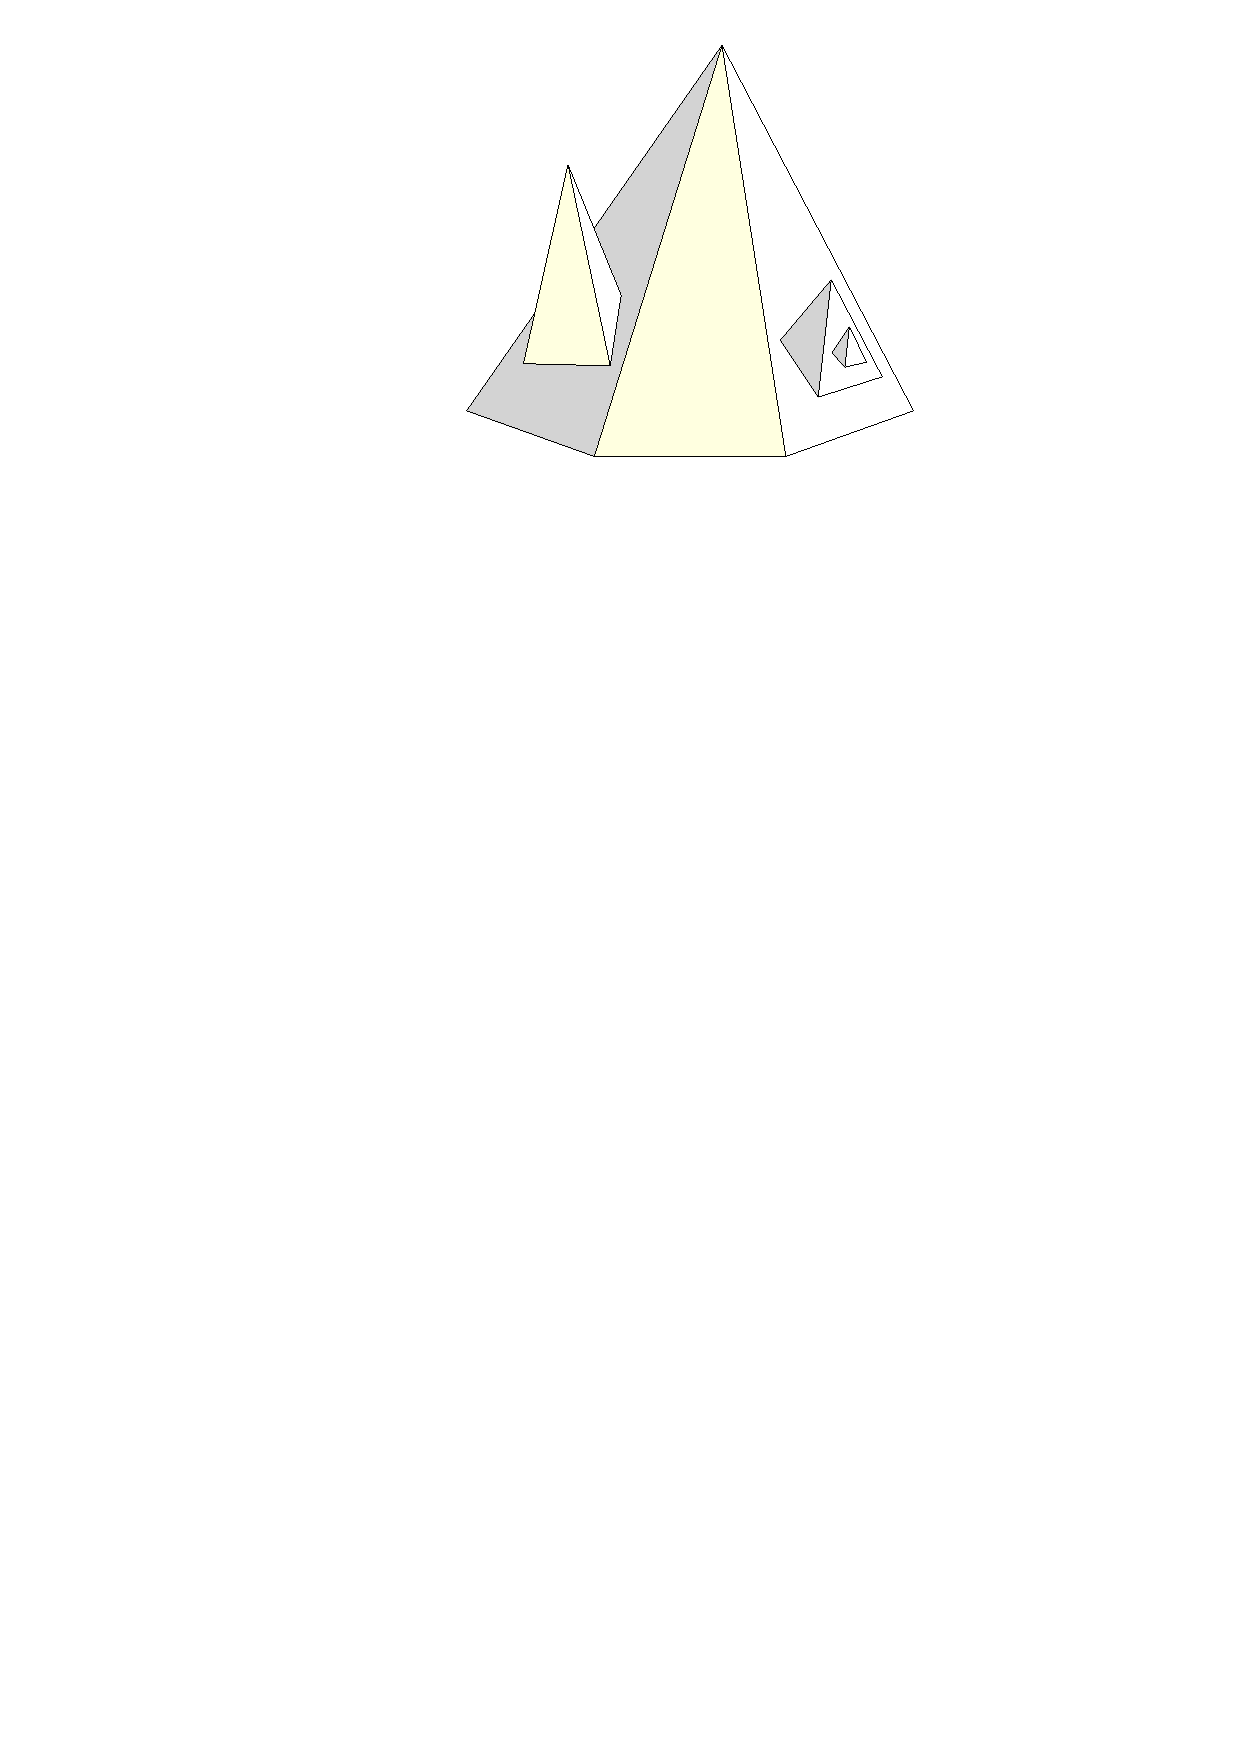
\includegraphics[width=.27\linewidth]{figs/spikey1}%
    \hspace{.35in}
    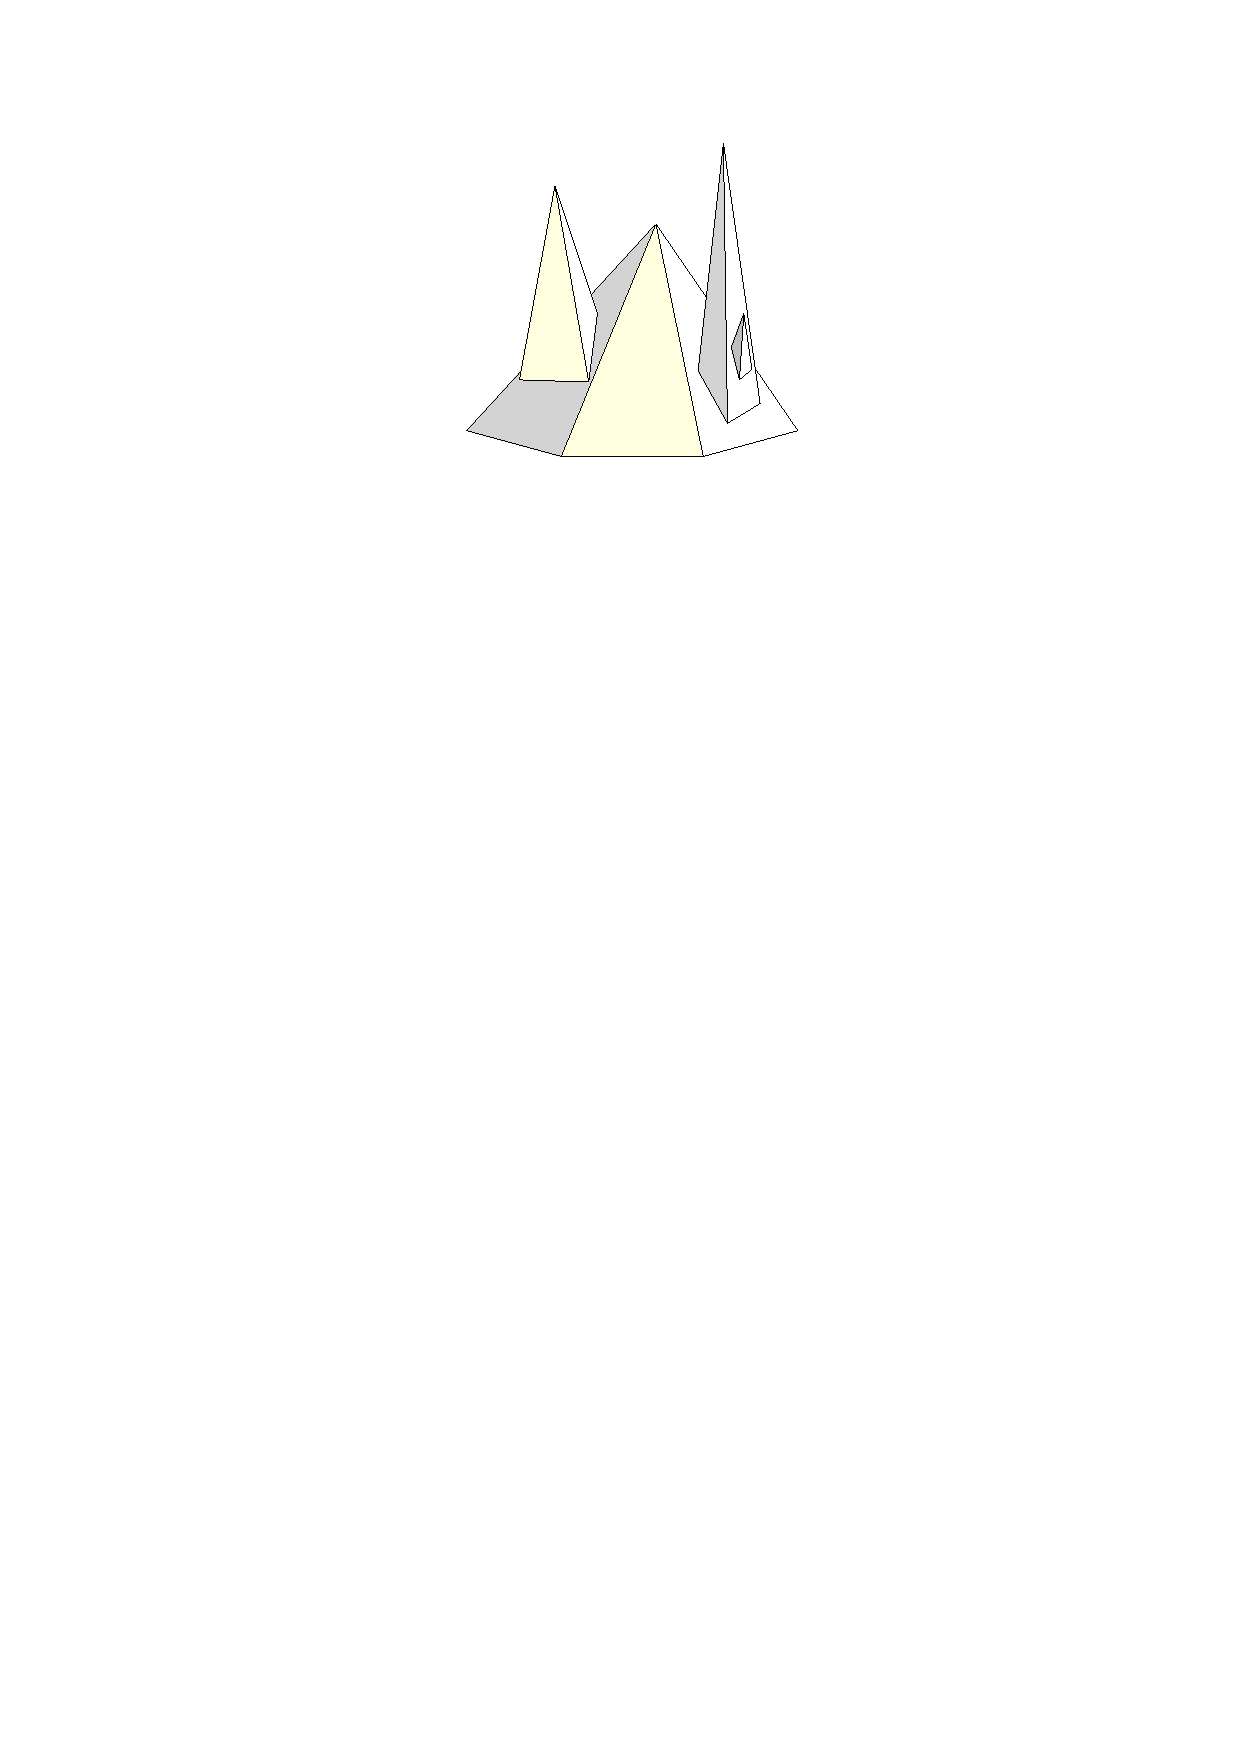
\includegraphics[width=.27\linewidth]{figs/spikey2}%
    \hspace{.4in}
    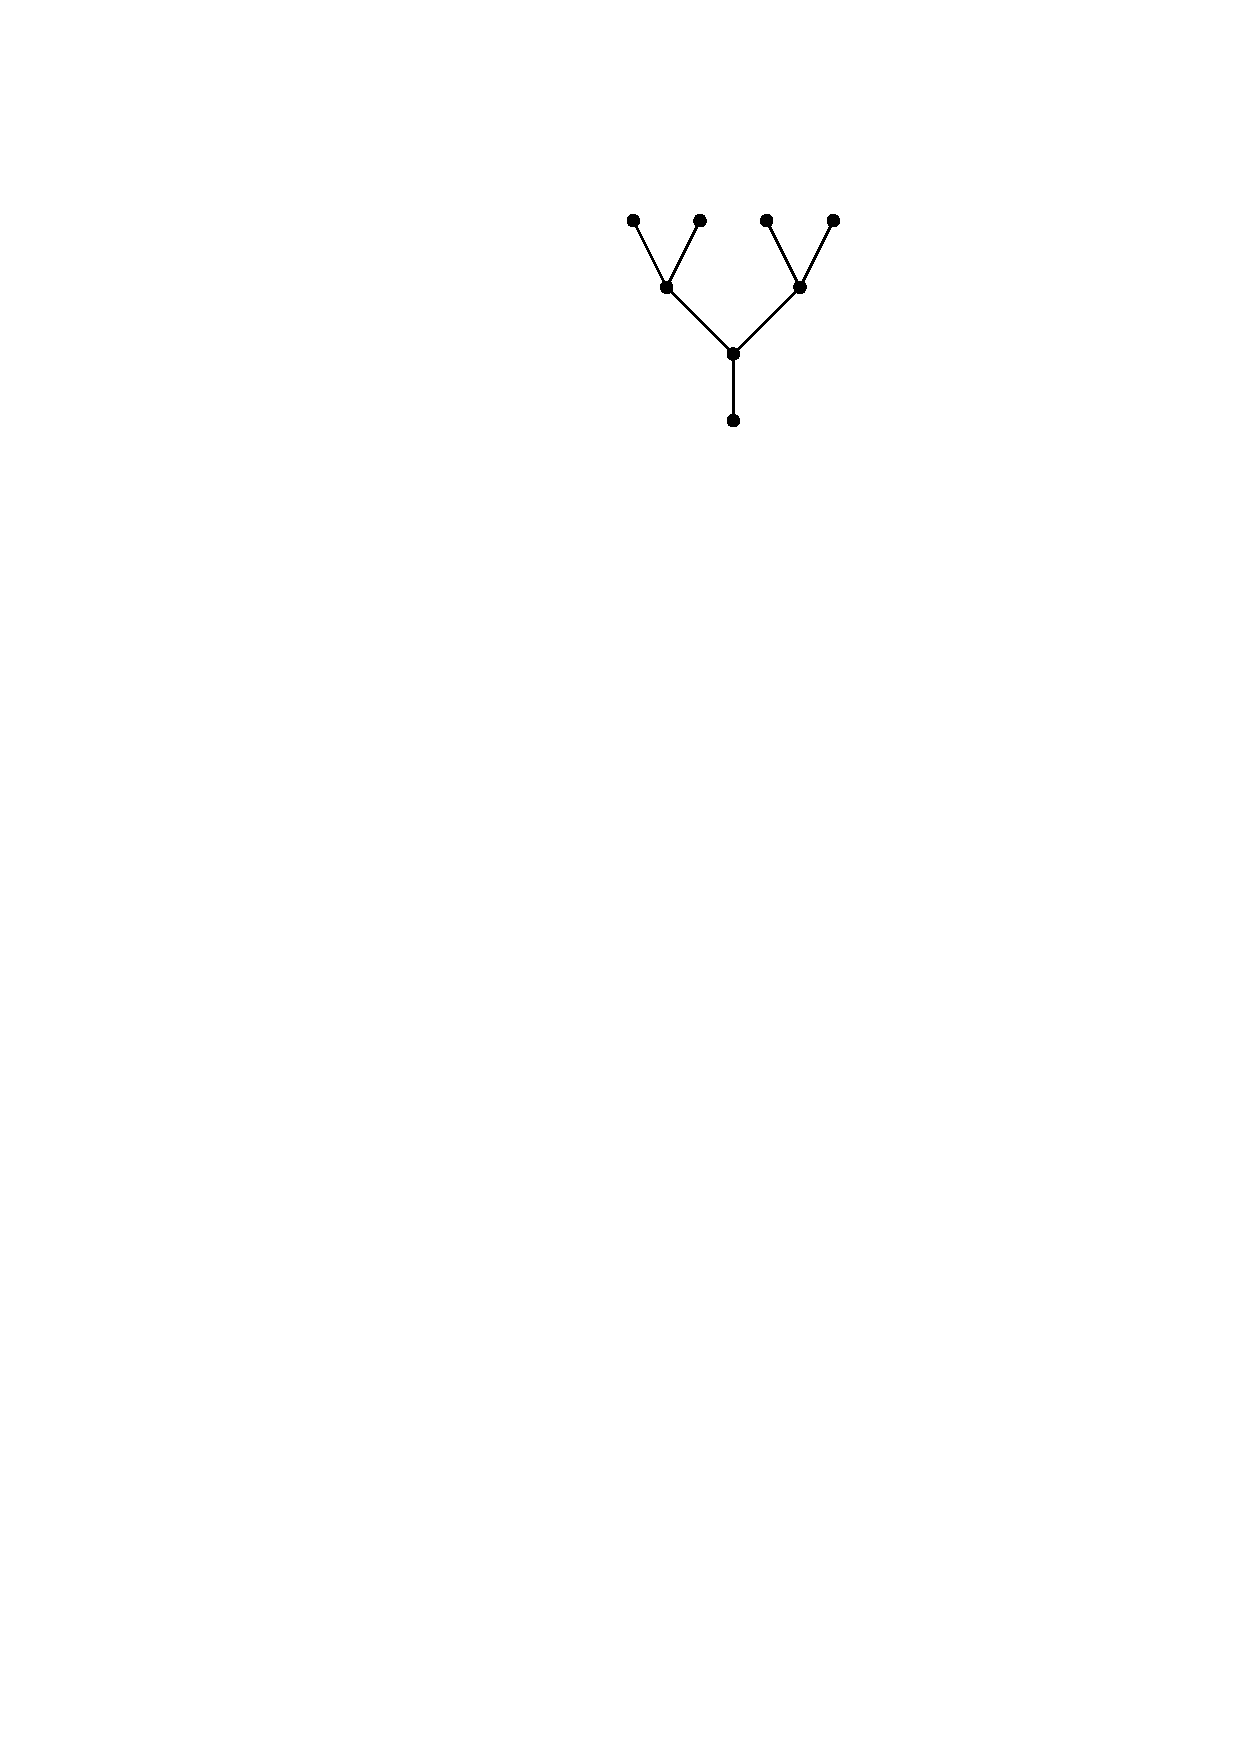
\includegraphics[width=.22\linewidth]{figs/spikeyTree}
    \caption{Two surfaces with different orderings of the maxima, but the same contour tree.}
    \label{fig:relative}
\end{figure}


\begin{figure}[h]\centering
    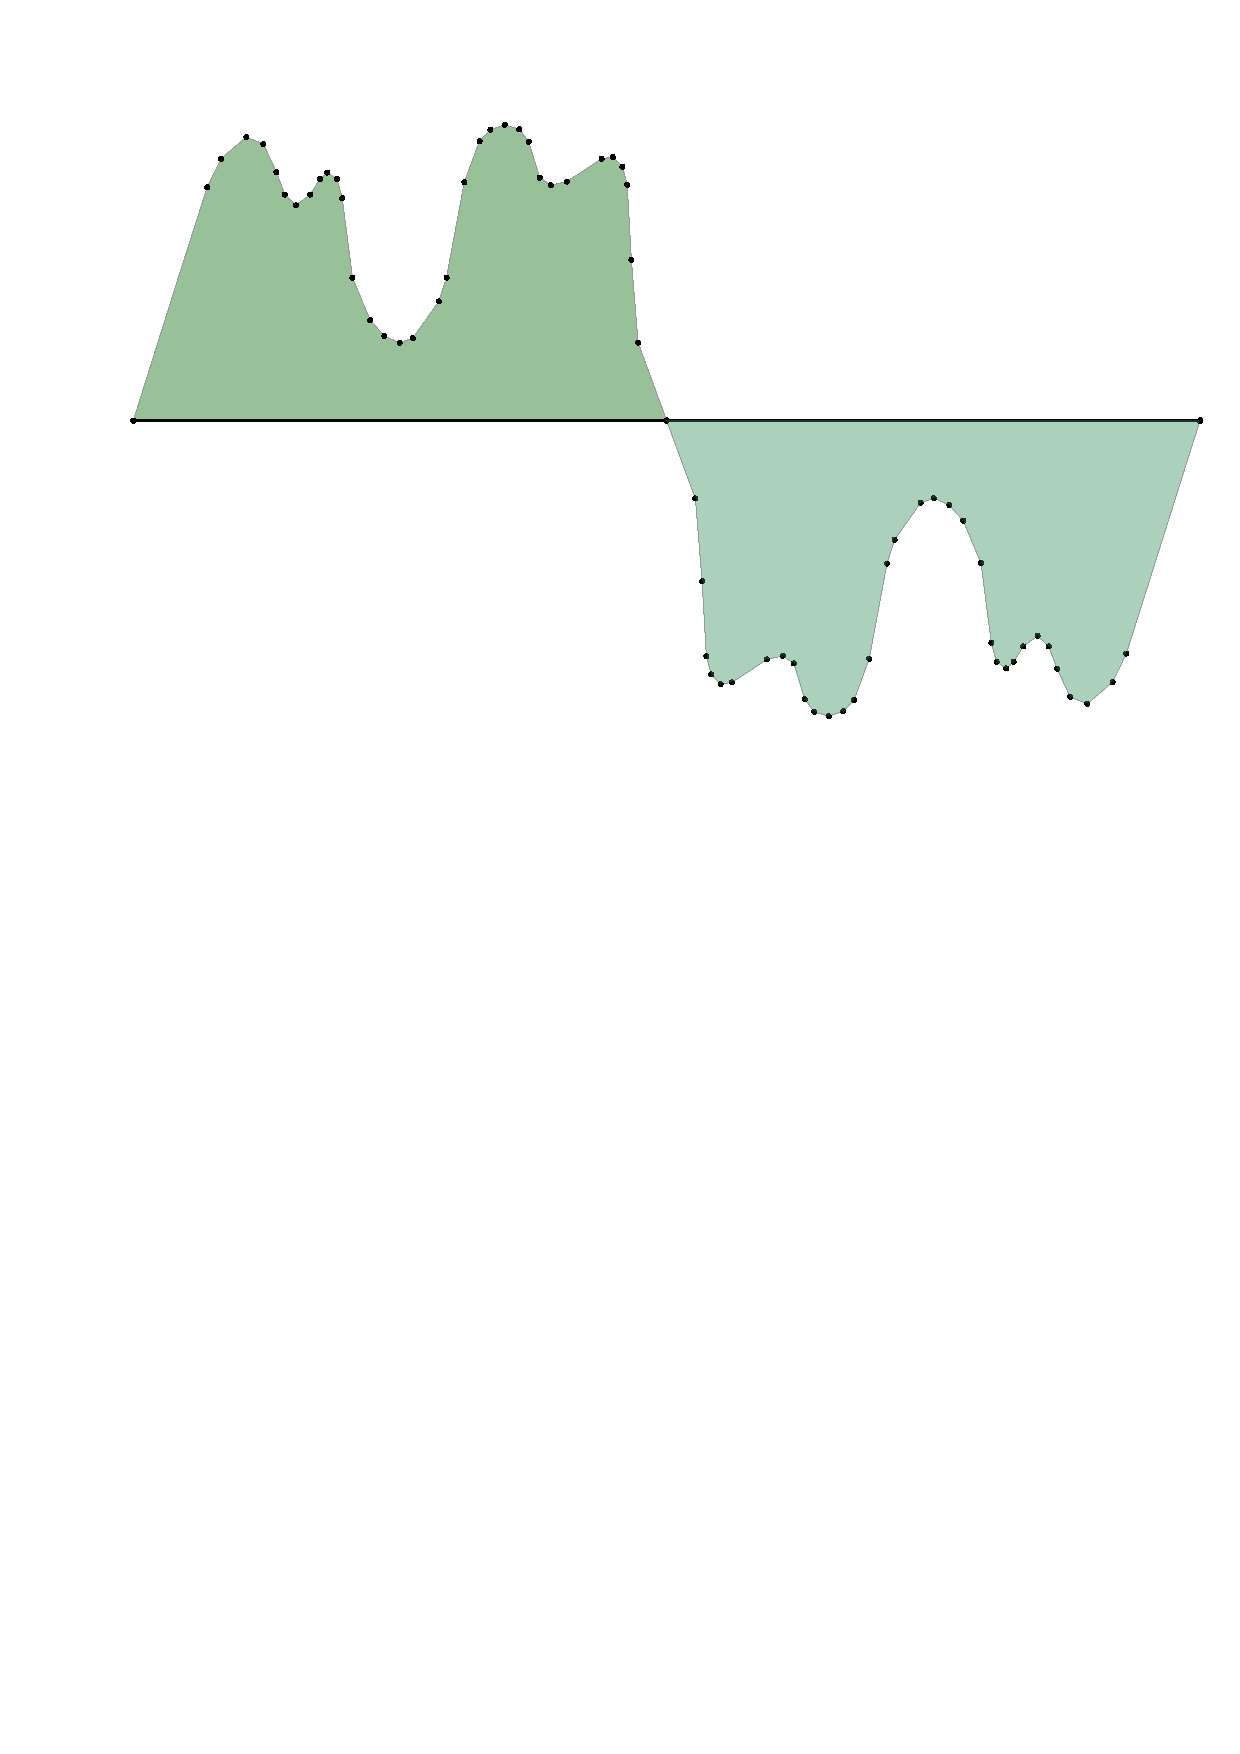
\includegraphics[width=.35\linewidth,height=.15\linewidth]{figs/balanced4}
    \hspace{.3in}
    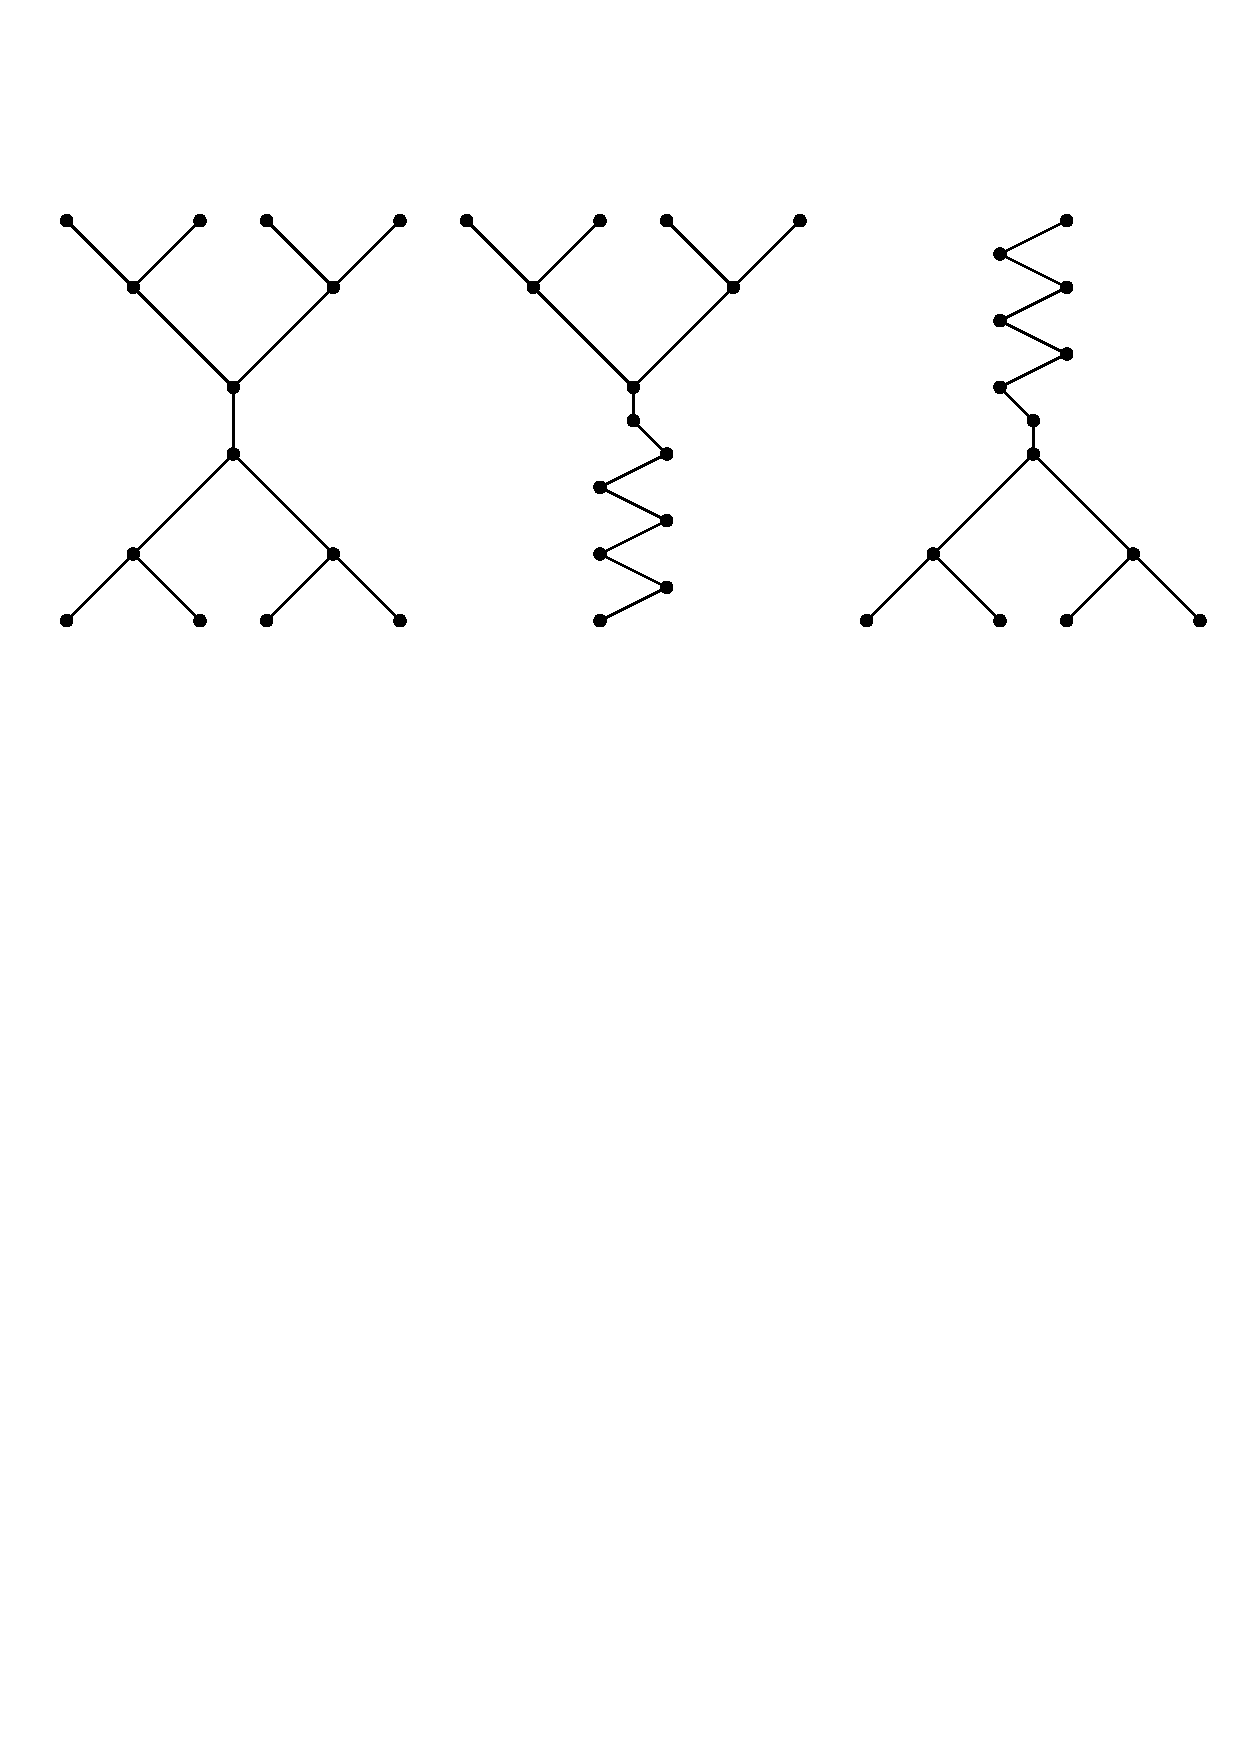
\includegraphics[width=.35\linewidth,height=.15\linewidth]{figs/trees}
    \caption{On left, a surface will a balanced contour tree, but whose join and split trees have long tails.  
    On right (from left to right), the contour, join and split trees.}
    \label{fig:sorting}
\end{figure}

% \paragraph{Organization.}  
% \Sec{basics} contains basic definition for contour trees.  In \Sec{approach} we give a high level overview and intuition for our approach 
% for computing contour trees.  \Sec{surgery} and \Sec{rain} describe how we break the intial input into nicely behaved (extemum dominant) pieces. 
% \Sec{extreme} shows that computing the contour tree for these nicely behaved pieces is roughly equivalent to computing the join tree. 
% \Sec{paint} contains our algorithm for computing join trees, which along with previous sections gives our algorithm for contour trees.  
% Finally, in \Sec{pathDecomp} and \Sec{lb} we relate the running time of our algorithm (providing upper and lower bounds) to a particular decomposition of the contour tree.

\section{Contour tree basics} \label{sec:basics}

We detail the basic definitions about contour trees. We follow the terminology of Chapter 6 of Carr's thesis \cite{c-tmi-04}.
All our assumptions and definitions
are standard for results in this area, though there is some variability in notation.
The input is a continuous piecewise-linear (PL) function $f:\MM \mapsto \RR$, where $\MM$ is a fully triangulated simplicial complex in $\RR^d$,
except for specially designated \emph{boundary facets}. So $f$ is defined only on the vertices of $\MM$,
and all other valued are obtained by interpolation. 

We assume that $f$ has distinct values on all vertices, except for boundaries,
as expressed in the following constraint.

\begin{definition} \label{def:bound} $f$ is \emph{boundary critical} if the following holds.
Consider a boundary facet $F$. All vertices of $F$ have the same function value. Furthermore, all
neighbors of $F$ not in $F$ either have all function values strictly greater or strictly less
than this value.
\end{definition}

This is convenient, as we can now assume that $f$ is defined on $\RR^d$. Any point inside a boundary facet
has a well-defined height, and this includes the infinite facet. 
We think of $d$ as constant, and assume that $\MM$ is represented in a data structure that allow constant-time traversals of neighboring simplices
in $\MM$ (e.g.~\cite{BoMa12}). (This is analogous to a DCEL for higher dimensions.)
Observe that $f:\MM \rightarrow \RR$ can be thought of as a $d$-dimensional simplicial complex living in $\RR^{d+1}$.
We can think of $f(x)$ as the ``height" of a point $x \in \MM$, and encoded in the representation of $\MM$. 

\begin{definition} \label{def:level} The level set at value $h$ is the set $\{x| f(x) = h\}$.
A contour is a maximal connected component of a level set. An $h$-contour is a contour where $f$-values are $h$.
\end{definition}

Note that a contour that does not contain a boundary is itself a simplicial complex of one dimension lower, and is represented (in our algorithms) as such.
We let $\delta, \eps$ denote infinitesimals. Let $B_\eps(x)$ denote a ball of radius $\eps$ around $x$, and let 
$f|B_\eps(x)$ be the restriction of $f$ to $B_\eps(x)$.


\begin{definition} \label{def:deg} The Morse up-degree of $x$ is the number of $(f(x) + \delta)$-contours in $f|B_\eps(x)$
as $\delta, \eps \rightarrow 0^+$. The Morse down-degree is the number of $(f(x) - \delta)$-contours in $f|B_\eps(x)$
as $\delta, \eps \rightarrow 0^+$.
\end{definition}

We categorize points depending on the local changes in topology.

\begin{definition} \label{def:points} A point $x$ is categorized as follows.
\begin{asparaitem}
	\item Regular: Both Morse up-degree and down-degrees are $1$.
	\item Maximum: Morse up-degree is $0$.
	\item Minimum: Morse down-degree is $0$.
	\item Morse Join: Morse up-degree is strictly greater than $1$.
	\item Morse Split: Morse down-degree is strictly greater than $1$.
\end{asparaitem}
Non-regular points are \emph{critical}. Morse joins and splits are \emph{saddles}.
Maxima and minima are \emph{extrema}.
\end{definition}


We use $\cV(f)$ to denote the set of critical points.
Because $f$ is piecewise-linear, all critical points are vertices in $\MM$. 
A value $h$ is called critical, if $f(v) = h$, for some $v \in \cV(f)$. 
The critical points are exactly where the topology of level sets change.
By assuming that our manifold is boundary critical, the vertices on a given boundary are either collectively all maxima or all minima.  
We abuse notation and refer to this entire set of vertices as a maxima or minima.


\begin{definition} \label{def:equiv} Two contours $\psi$ and $\psi'$ are equivalent 
if the following holds. There exists an $f$-monotone path $p$ connecting a point in $\psi$ to $\psi'$,
such that no $x \in p$ belongs to a critical contour.
\end{definition}

These give the \emph{contour classes}. By continuity, a regular point is present on a single contour,
and we can partition the regular contours into these classes. Every such class maps to intervals
of the form $(f(x_i),f(x_j))$, where $x_i, x_j$ are critical points. Such a class is said
to be created at $x_i$ and destroyed at $x_j$. 

\begin{definition} \label{def:tree} The contour tree is the graph on vertex set $\cV$, where
edges are formed as follows. For every contour class that is created at $v_i$ and destroyed $v_j$,
there is an edge $(v_i,v_j)$. (Conventionally, edges are directed from higher to lower function value.)
\end{definition}

We denote the contour tree of $\MM$
by $\reeb(\MM)$. The corresponding node and edge sets are denoted as $\cV(\cdot)$ and $\cE(\cdot)$.
It is not immediately obvious that this graph is a tree, but alternate definitions of the contour tree
in~\cite{csa-cctad-00} imply this is a tree. 
Since this tree has height values associated with the vertices, we can talk about up-degrees and down-degrees in $\reeb(\MM)$.
We assume there are no ``multi-saddles", so up and down-degrees are at most $2$, and the total degree is at most $3$. 
This is again a standard assumption in topological algorithms and can be achieved by vertex unfolding (Section 6.3 in~\cite{HaEd10}).

\subsection{Some technical remarks}

The $(f(x)+\delta)$-contours in $f|_{B_\eps(x)}$ given by \Def{deg} might actually be the same
contour in $f$. The up-degree (as opposed to \emph{Morse} up-degree) is defined as the number of $(f(x)+\delta)$-contours
that intersect $B_\eps(x)$, a potentially smaller number. This up-degree
is exactly the up-degree of $x$ in $\reeb(\MM)$. (Analogously, for down-degree.)
When the Morse up-degree is $2$ but the up-degree is $1$, the topology of the level set changes but not by the number of connected components changing.
For example, when $d=3$ this is equivalent to the contour gaining a handle.
When $d=2$, this distinction is not necessary, since any point with $>1$
Morse degree will have $>1$ degree in $\reeb(\MM)$.

As Carr points out in Chapter 6 of his thesis, the term contour tree can be used for a family of related structures.
Every vertex in $\MM$ is associated with an edge in $\reeb(\MM)$, and sometimes the
vertex is explictly placed in $\reeb(\MM)$ (by subdividing the respective edge). This is referred
to as augmenting the contour tree, and it is common to augment $\reeb(\MM)$ will all vertices.
Alternatively, one can smooth out all vertices of up-degree and down-degree $1$ to get the
unaugmented contour tree. (For $d=2$, there are no such vertices in $\reeb(\MM)$.) 
The contour tree of \Def{tree} is the typical definition in all results on output-sensitive
contour trees, and is the smallest tree that contains all the topological changes
of level sets. \Thm{main-alg} is applicable for any augmentation of $\reeb(\MM)$ with a predefined
set of vertices, though we will not delve into these aspects in this paper.


\section{A tour of the contour tree algorithm} \label{sec:approach}

Our final algorithm is quite technical and has numerous moving parts. This section
provides a high level view of the entire result, and highlights the main ideas
and intuition. 
\SubmitVer{The full version with all the details can be found in the appendix.}
It is helpful to keep the $d=2$ case in mind, so the input is just a triangulated
terrain. In the interest of presentation, the definitions and theorem statements in this section will
slightly differ from those in the main body. They may also differ from the original definitions proposed
in earlier work. 

\paragraph{Do not globally sort:} Arguably, the starting point for this work is \Fig{relative}. We have two terrains
with exactly the same contour tree, but different orderings of (heights of) the critical points.
Turning it around, we cannot deduce the full height ordering of critical points from the contour tree. Therefore, clearly
sorting all critical points is computationally unnecessary for constructing the contour tree.
In \Fig{sorting}, the contour tree basically consists of two balanced binary trees, one of the joins,
another of the splits. Again, it is not necessary to know the relative ordering between the mounds
on the left (or among the depressions on the right) to compute the contour tree. Yet some ordering
information is necessary: on the left, the little valleys are higher than the big central valley,
and this is reflected in the contour tree. More generally, leafs paths in the contour tree have points
in sorted order, but incomparable points in the tree are unconstrained.
How do we sort exactly what is required, without knowing the contour tree in advance?

\subsection{Breaking $\MM$ into simpler pieces} \label{sec:break}

Let us begin with the algorithm of Carr, Snoeyink, and Axen~\cite{csa-cctad-00}. The key insight is to build
two different trees, called the join and split trees, and then merge them together into the contour tree.
Consider sweeping down via the hyperplane $x_{d+1} = h$ and taking the \emph{superlevel} sets. These 
are the connected components of the portion of $\MM$ above height $h$. For a terrain, the superlevel
sets are a collection of ``mounds". As we sweep downwards, these mounds keep joining each other,
until finally, we end up with all of $\MM$. The join tree tracks exactly these events. 
Formally, let $\MM^+_v$ denote the simplicial complex induced on the subset of 
vertices which are higher than $v$.

\begin{definition} 
\label{def:int-criticalJoin}
The critical join tree $\jc(\MM)$ is built on the set $\cV$ of all critical points. 
The directed edge $(u,v)$ is present when $u$ is the smallest valued vertex in $\cV$ in a connected component of $\MM^+_v$
and $v$ is connected to this component (in $\MM$). 
\end{definition}

(Abusing notation, we just call this the join tree.)
Refer to \Fig{sorting} for the join tree of a terrain. Note that nothing happens at splits, but these
are still put as vertices in the join tree. They simply form a long path. The split tree
is obtained by simply inverting this procedure, sweeping upwards and tracking sublevel sets.

A major insight of~\cite{csa-cctad-00} is an ingeniously simple linear time procedure to construct
the contour tree from the join and split trees. So the bottleneck is computing these trees. Observe
in \Fig{sorting} that the split vertices form a long path in the join tree (and vice versa). Therefore, constructing
these trees forces a global sort of the splits, an unnecessary computation for the contour tree. Unfortunately, in general (i.e. unlike \Fig{sorting}) 
the heights of joins and splits may be interleaved in a complex manner, and hence the final merging of~\cite{csa-cctad-00}
to get the contour tree requires having the split vertices in the join tree. Without
this, it is not clear how to get a consistent view of both joins and splits, required for the contour tree.

Our aim is to break $\MM$ into smaller pieces, where this unnecessary computation can be avoided.


\paragraph{Contour surgery:} We first need a divide-and-conquer lemma. Any contour $\phi$ can be associated
with an edge $e$ of the contour tree. Suppose we ``cut" $\MM$ along this contour. We prove that $\MM$
is split into two disconnected pieces, such the contour trees of these pieces is obtained
by simply cutting $e$ in $\reeb(\MM)$. Alternatively, the contour trees of these pieces can
be glued together to get $\reeb(\MM)$. This is not particularly surprising, and is fairly easy to prove
with the right definitions. The idea of loop surgery has been used to reduce Reeb graphs to contour trees~\cite{TiGySi09,DoNa13}.
Nonetheless, our theorem appears to be new and works for all dimensions.


\begin{figure}[h]\centering
    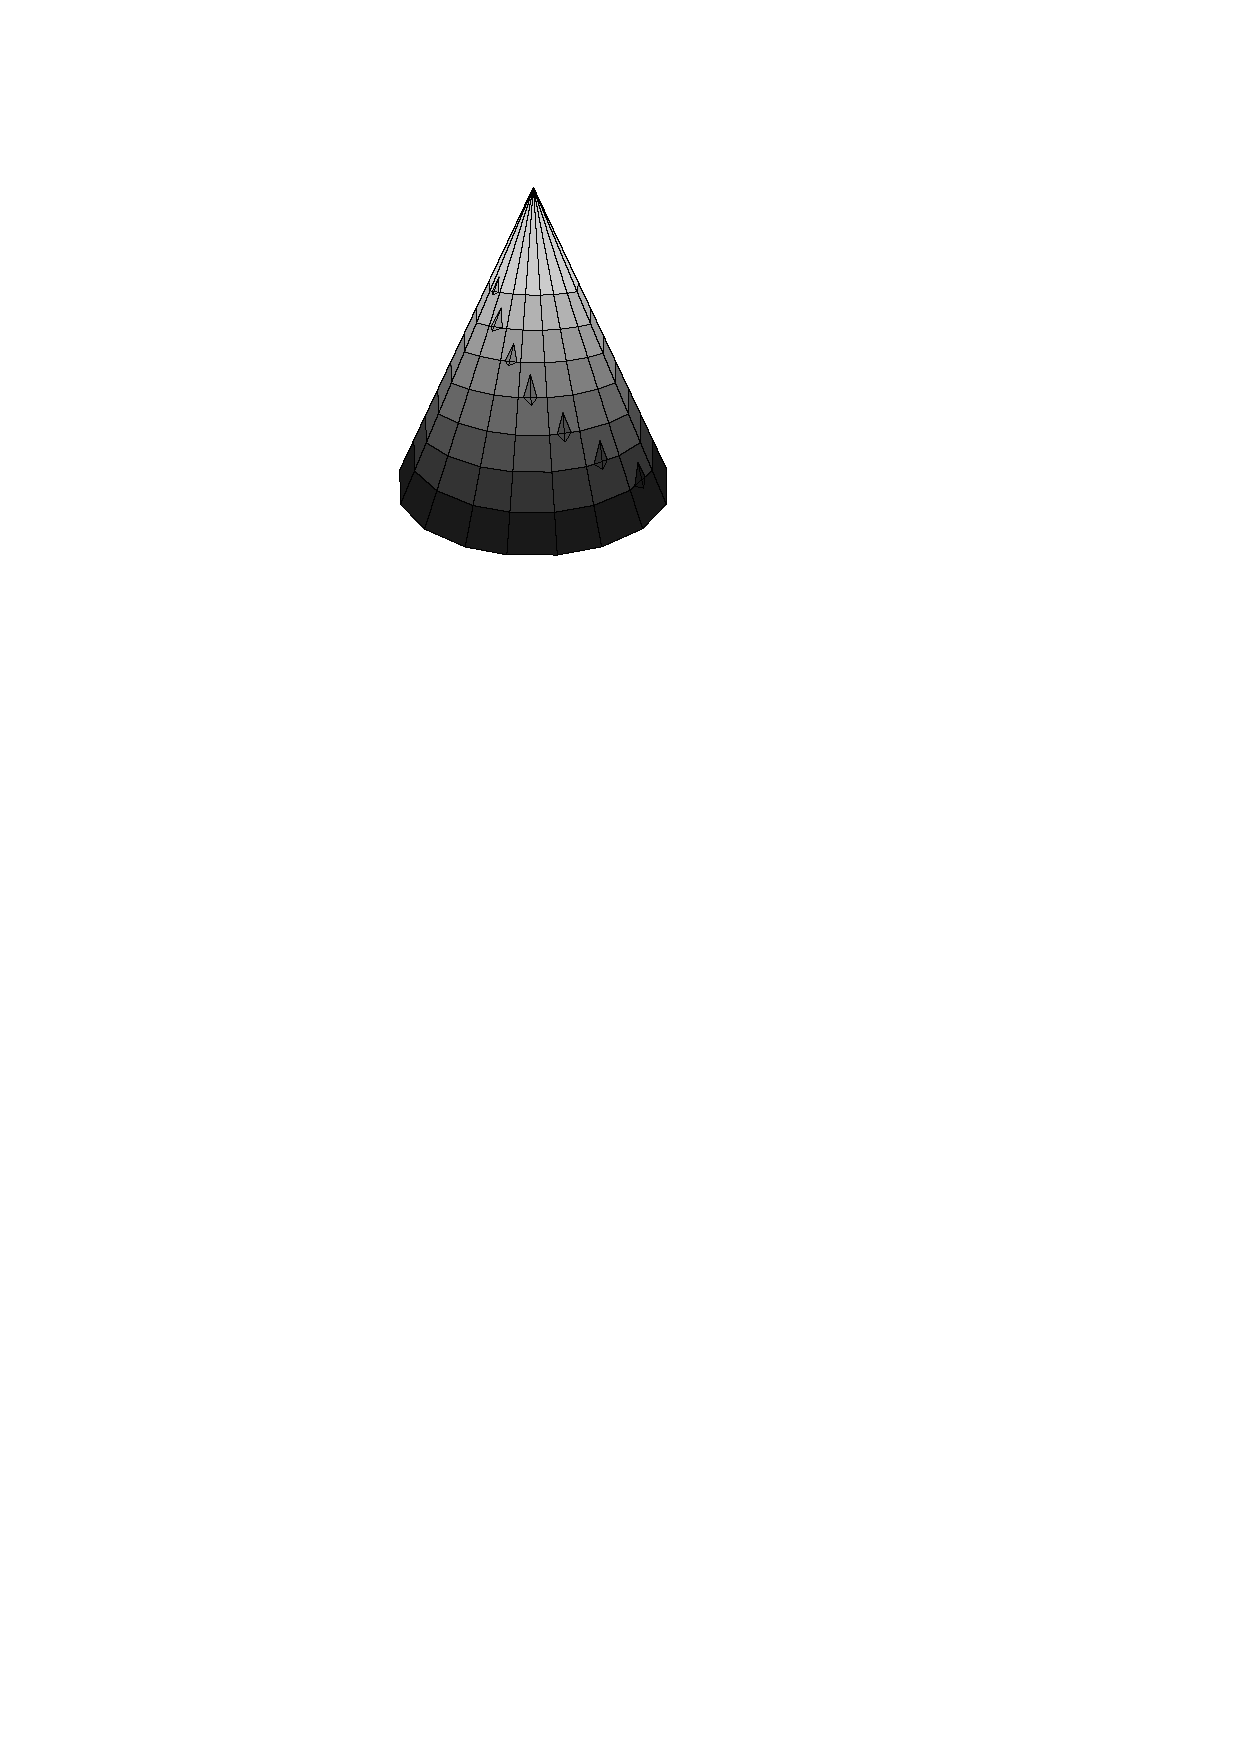
\includegraphics[width=.18\linewidth]{figs/tent2}%
    \hspace{.9in}
    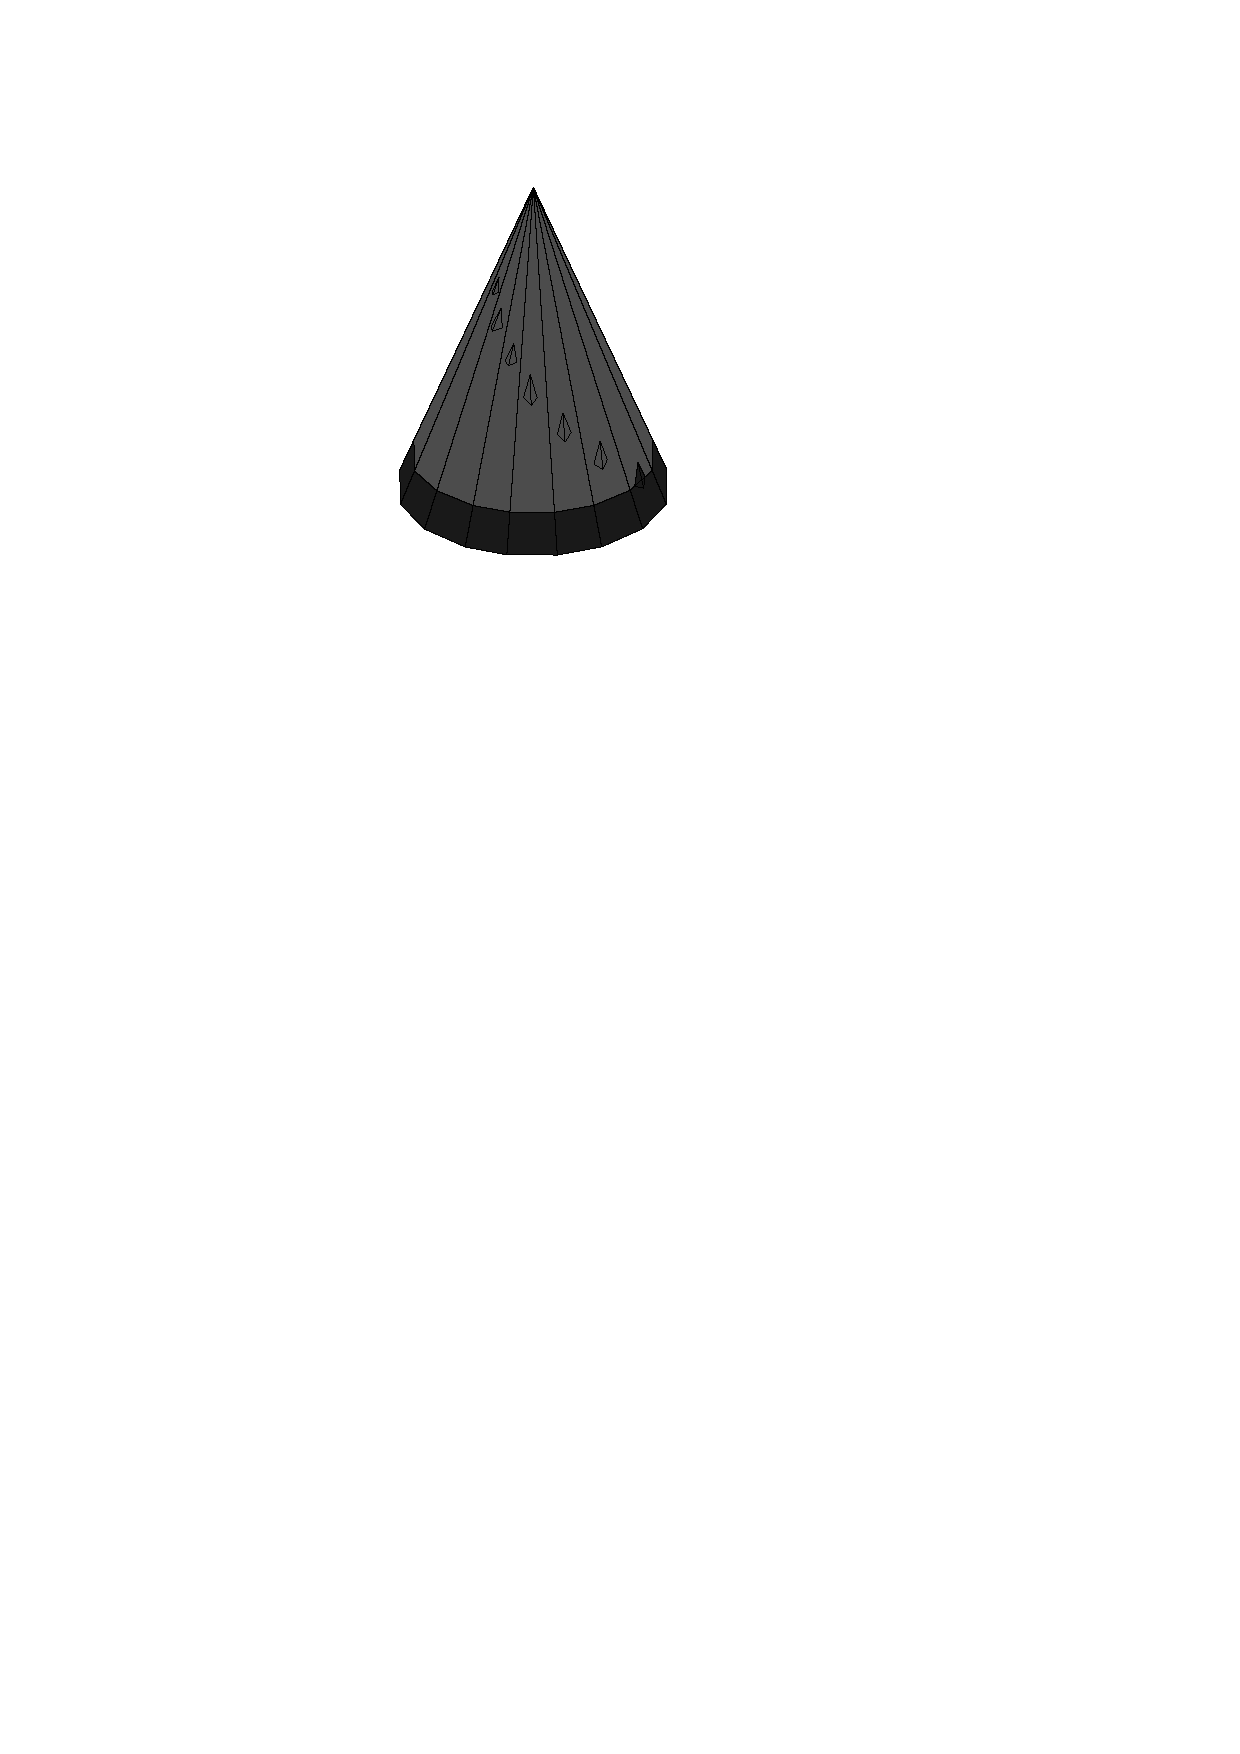
\includegraphics[width=.18\linewidth]{figs/tent1}
    \caption{On left, downward rain spilling only (each shade of gray represents a piece created by each different spilling), producing a grid.  
    Note we are assuming raining was done in reverse sorted order of maxima.  
    On right, flipping the direction of rain spilling.}
    \label{fig:order}
\end{figure}

\paragraph{Cutting $\MM$ into extremum dominant pieces:} We define a simplicial complex
endowed with a height to be \emph{minimum dominant} if there only exists a single minima.
(Our real definition is more complicated, and involves simplicial complexes
that allow additional ``trivial'' minima.)
In such a complex, there exists a non-ascending path from any point to this unique minima.
Analogously, we can define maximum dominant simplicial complexes,
and both are collectively called extremum dominant.

We will cut $\MM$ into disjoint extremum dominant pieces, in linear time.
The best way to think of our procedure is a meteorology analogy. Take an arbitrary maxima $x$,
and imagine torrential rain at the maxima. The water flows down, wetting any point that has a non-ascending path 
from $x$. We end up with two portions, the wet part of $\MM$ and the dry part. This is similar
to \emph{watershed} algorithms used for image segmentation~\cite{RoMe00}. The wet part is obviously connected,
while there may be numerous disconnected dry parts. The interface between the dry and wet parts
is a set of contours, given by the ``water line". The wet part is clearly maximum dominant, since all
wet points have a non-descending path to $x$. So we can simply cut along the interface
contours to get the wet maximum dominant piece $\MM'$. By our contour surgery theorem,
we are left with a set of disconnected dry parts, and we can recur this procedure on them.

But here's the catch. Every time we cut $\MM$ along a contour, we potentially increase
the complexity of $\MM$. Water flows in the interior of facets, and the interface will naturally
cut some facets. Each cut introduces new vertices, and a poor choice of repeated raining leads
to a large increase in complexity. Consider the left of \Fig{order}. Each raining produces a single
wet and dry piece, and each cut introduces many new vertices. If we wanted to partition this terrain into 
maximum dominant simplicial complexes, the final complexity would be forbiddingly large.

A simple trick saves the day. Unlike reality, we can choose rain to flow solely downwards or solely upwards.
Apply the procedure above to get a single wet maximum dominant $\MM'$ and a set of dry pieces.
Observe that a single dry piece $\NN$ is boundary critical with the newly introduced boundary $\phi$ (the wet-dry interface) behaving as a minima.
So we can rain upwards from this minima, and get a \emph{minimum dominant} portion $\NN'$.
This ensures that the new interface (after applying the procedure on $\NN$) does not
cut any facet previously cut by $\phi$.
For each of the new dry pieces, the newly introduced boundary is now a maximum. So we rain downwards from there.
More formally, we alternate between raining upwards and downwards as we go down the recursion tree.
We can prove that an original facet of $\MM$ is cut at most once, so the final complexity can be bounded.
In \Fig{order}, this procedure would yield two pieces, one maximum dominant, and one minimum dominant.

Using the contour surgery theorem previously discussed, we can build the contour tree of $\MM$
from the contour trees of the various pieces created. All in all, we prove the following theorem.

\begin{theorem} \label{thm:int-rain} There is an $O(N)$ time procedure that cuts $\MM$ into extremum dominant simplicial complexes
$\MM_1, \MM_2, \ldots$. Furthermore, given the set of contour trees $\{\cC(\MM_i)\}$, $\cC(\MM)$ can be constructed in $O(N)$ time.
\end{theorem}

\paragraph{Extremum dominance simplifies contour trees:} We will focus on minimum dominant simplicial complexes $\MM$. By \Thm{int-rain}, it suffices
to design an algorithm for contour trees on such inputs. 
For the $d=2$ case, it helps to visualize such an input as a terrain with no minima,
except at a unique boundary face (think of a large boundary triangle that is the boundary).
All the valleys in such a terrain are necessarily joins, and there can be no splits. Look
at \Fig{sorting}. The portion on the left is minimum dominant in exactly this fashion.
%Water poured at any critical point must flow to the boundary, and the entire wet portion is connected.
More formally, $\MM^-_v$ is connected for all $v$, so there are no splits.

We can prove that the split tree is just a path, and the contour tree is exactly
the join tree. The formal argument is a little involved, and we employ the merging procedure
of~\cite{csa-cctad-00} to get a proof. We demonstrate that the merging procedure will
actually just output the join tree, so we do not need to actually compute the split tree.
(The real definition of minimum dominant is a little more complicated,
so the contour tree is more than just the join tree. But computationally, it suffices
to construct the join tree.)

We stress the importance of this step for our approach. Given the algorithm of~\cite{csa-cctad-00},
one may think that it suffices to design faster algorithms for join trees. But this
cannot give the sort of optimality we hope for. Again, consider \Fig{sorting}. Any algorithm
to construct the true join tree must construct the path of splits, which implies
sorting all of them. It is absolutely necessary to cut $\MM$ into pieces where the cost
of building the join tree can be related to that of building $\cC(\MM)$.

\subsection{Join trees from painted mountaintops} \label{sec:join-paint}

Arguably, everything up to this point is a preamble for the main result: a faster
algorithm for join trees. Our algorithm does not require the input to be extremum
dominant. This is only required to relate the join trees to the contour tree of initial input $\MM$.
For convenience, we use $\NN$ to denote the input here. Note that as defined in \Def{int-criticalJoin},
the join tree is defined purely combinatorially in terms of the 1-skeleton (the underlying graph) of $\NN$.

The join tree $\jc(\NN)$ is a rooted tree with the dominant minimum at the root, and we direct edges downwards (towards the root). So it makes sense to talk
of comparable vs incomparable vertices.
We arrive at the primary challenge: how to sort only those critical points that are comparable, without
constructing the join tree? The join tree algorithm of~\cite{csa-cctad-00} is a typical event-based
computational geometry algorithm. We have to step away from this viewpoint to avoid the global sort.

The key idea is \emph{paint spilling}. Start with each maxima having a large can of paint, with distinct
colors for each maxima. In arbitrary order, we spill paint from each maxima, wait till it flows down,
then spill from the next, etc. Paint is viscous, and only flows down edges. \emph{It does not
paint the interior of facets.} That is, this process is restricted to the 1-skeleton of $\NN$.
Furthermore, our paints do not mix, so each edge receives a unique color, which is decided by the first
paint to reach it. 

\begin{definition} \label{def:paint} Let the 1-skeleton of $\NN$ have edge set $E$ and maxima $X$.
A  \emph{painting} of $\NN$ is a map $\chi:X \cup E \mapsto [|X|]$ with the following property. 
 Consider an edge $e$. There exists a descending path from some maximum $x$ to $e$
	consisting of edges in $E$, such that all edges along this path have the same color as $x$. 

An \emph{initial} painting has the additional property that the restriction $\chi:X \mapsto [|X|]$ is a bijection.
\end{definition}

Note that a painting only colors edges, not vertices. Our definition also does not require the timing aspect
of iterating over colors, though that is one way of painting $\NN$. We begin with an initial painting, since all maxima
colors are distinct. A few comments on paint vs water. The interface between two regions of different color
is \emph{not} a contour, and is actually difficult to characterize. So we cannot apply the divide-and-conquer
approach of contour surgery. On the other hand, painting does not cut $\NN$, so there is no increase in complexity.
Clearly, an initial painting can be constructed in $O(N)$ time. This is the tradeoff between water and paint.
Water allows for an easy divide-and-conquer, at the cost of more complexity in the input. For an extremum
dominant input, using water to divide the input $\NN$ raises the complexity too much.

Our algorithm incrementally builds $\jc(\MM)$ from the leaves (maxima) to the root (dominant minimum). 
We say that vertex $v$ is \emph{touched} by color $c$, if there is a $c$-colored edge with lower endpoint $v$.
Let us focus on an initial painting, where the colors have 1-1 correspondence with the maxima. Refer to the left part of \Fig{colors}.
Consider two sibling leaves $\ell_1, \ell_2$ and their common parent $v$. The leaves are maxima,
and $v$ is a join that ``merges" $\ell_1, \ell_2$. 
In that case, there are ``mounds" corresponding to $\ell_1$ and $\ell_2$ that merge
at a valley $v$. Suppose this was the entire input, and $\ell_1$ was colored blue and $\ell_2$ was colored red. 
Both the mounds are colored completely blue or red, while $v$ is touched by both colors.
So this indicates that $v$ joins the blue maxima and red maxima in $\jc(\MM)$.

This is precisely how we hope to exploit the information in the painting. We prove later that
when some join $v$ has all incident edges with exactly two colors, the corresponding maxima (of those colors) are exactly
the children of $v$ in $\jc(\MM)$. To proceed further, we ``merge" the colors red and blue into a new color, purple. In other words,
we replace all red and blue edges by purple edges. This indicates that the red and blue maxima have been
handled. Imagine flattening the red and blue mounds until reaching $v$, so that the former join $v$
is now a new maxima. Suppose purple paint was poured from $v$. In terms of $\jc(\MM)$, this
is equivalent to removing leaves $\ell_1$ and $\ell_2$, making $v$ a new leaf.
Alternately, $\jc(\MM)$ has been constructed up to $v$, and it remains to determine $v$'s parent.
The merging of the colors is not explicitly performed as that would be too expensive; we maintain a union-find
data structure for that.

Of course, things are more complicated when there are other mounds. There may be a yellow mound,
corresponding to $\ell_3$ that joins with the blue mound higher up at some vertex $u$ (see the right part of \Fig{colors}). In $\jc(\MM)$, $\ell_1$ and $\ell_3$
are sibling leaves, and $\ell_2$ is a sibling of some ancestor of these leaves. So we cannot
merge red and blue, until yellow and blue merge. Naturally, we use priority queues to handle this issue.
We know that $u$ must also be touched by blue. So all critical vertices touched by blue
are put into a priority queue keyed by height, and vertices are handled in that order.

\begin{figure}[h]\centering
    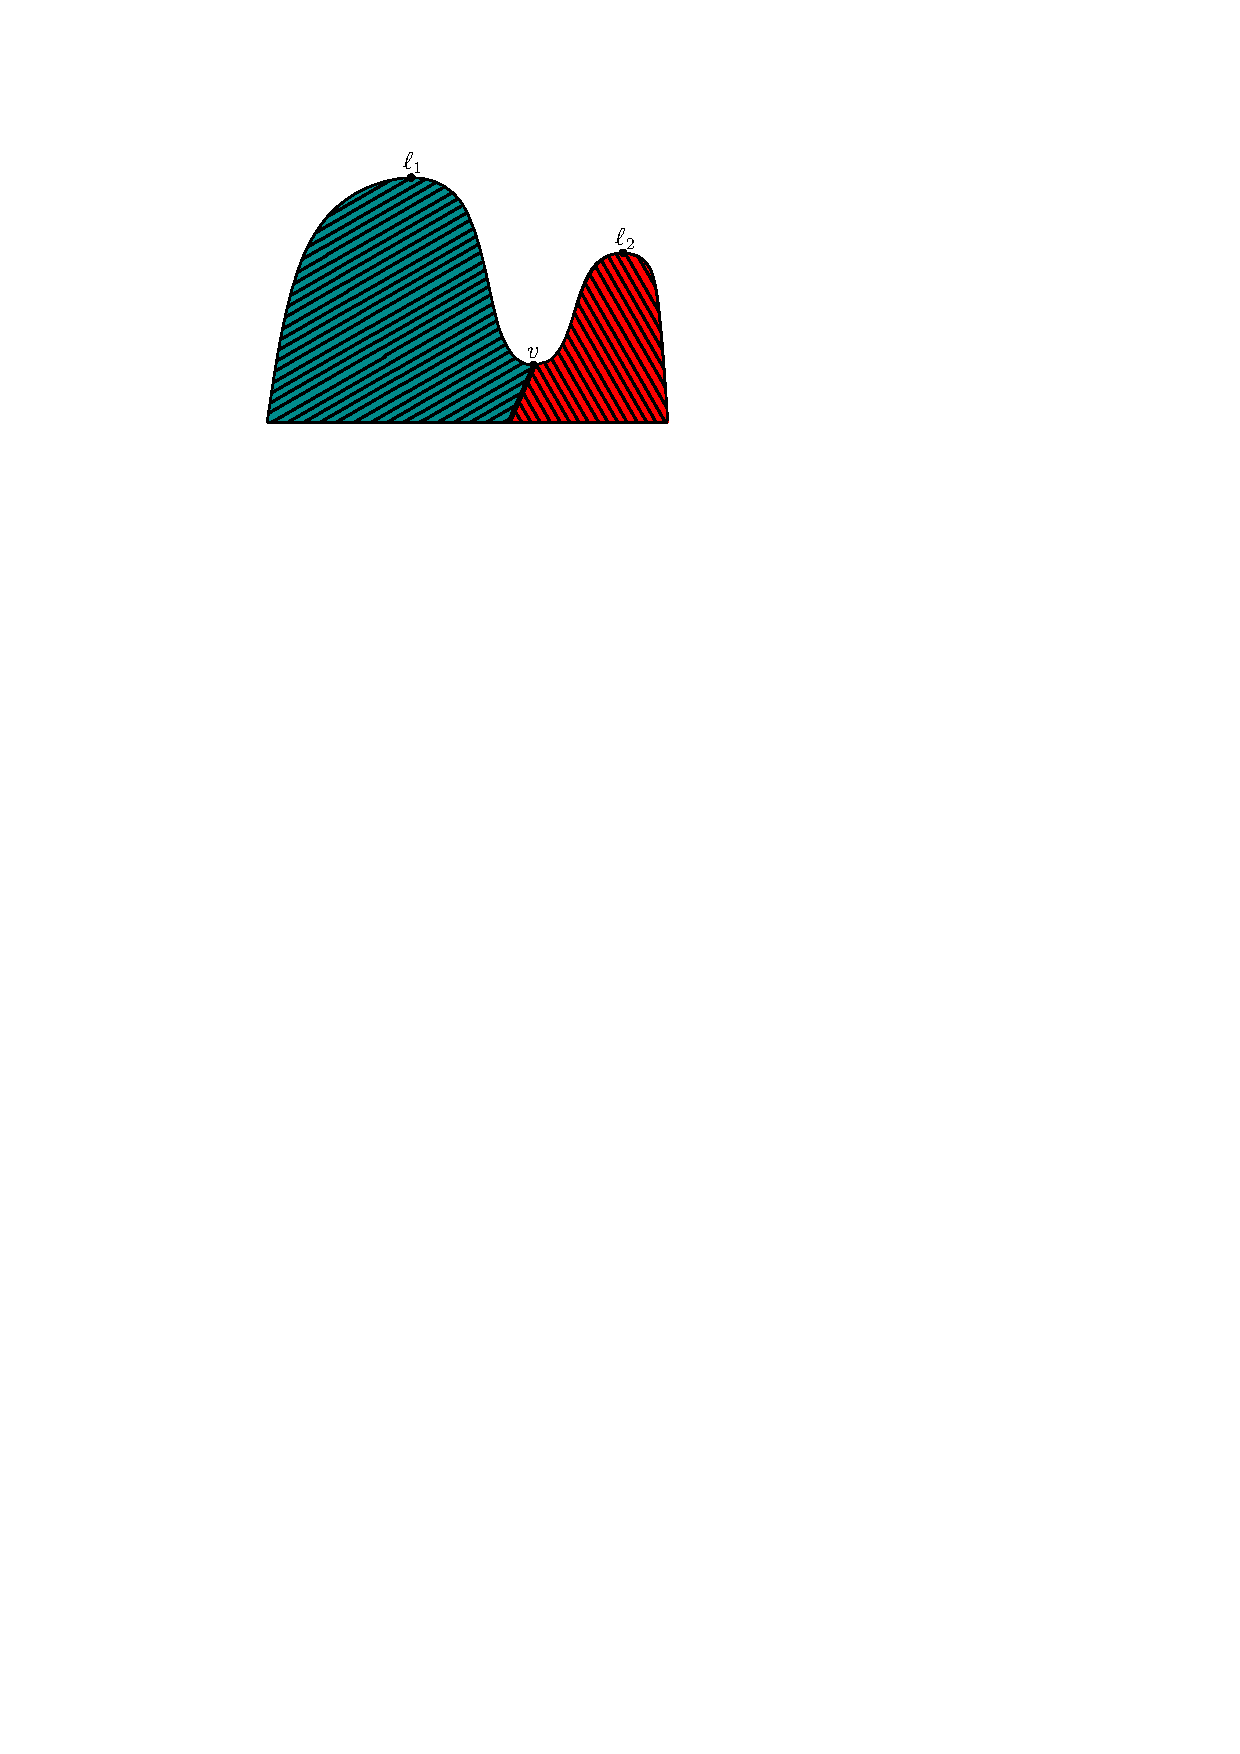
\includegraphics[width=.25\linewidth]{figs/redBlue}%
    \hspace{.07in}
    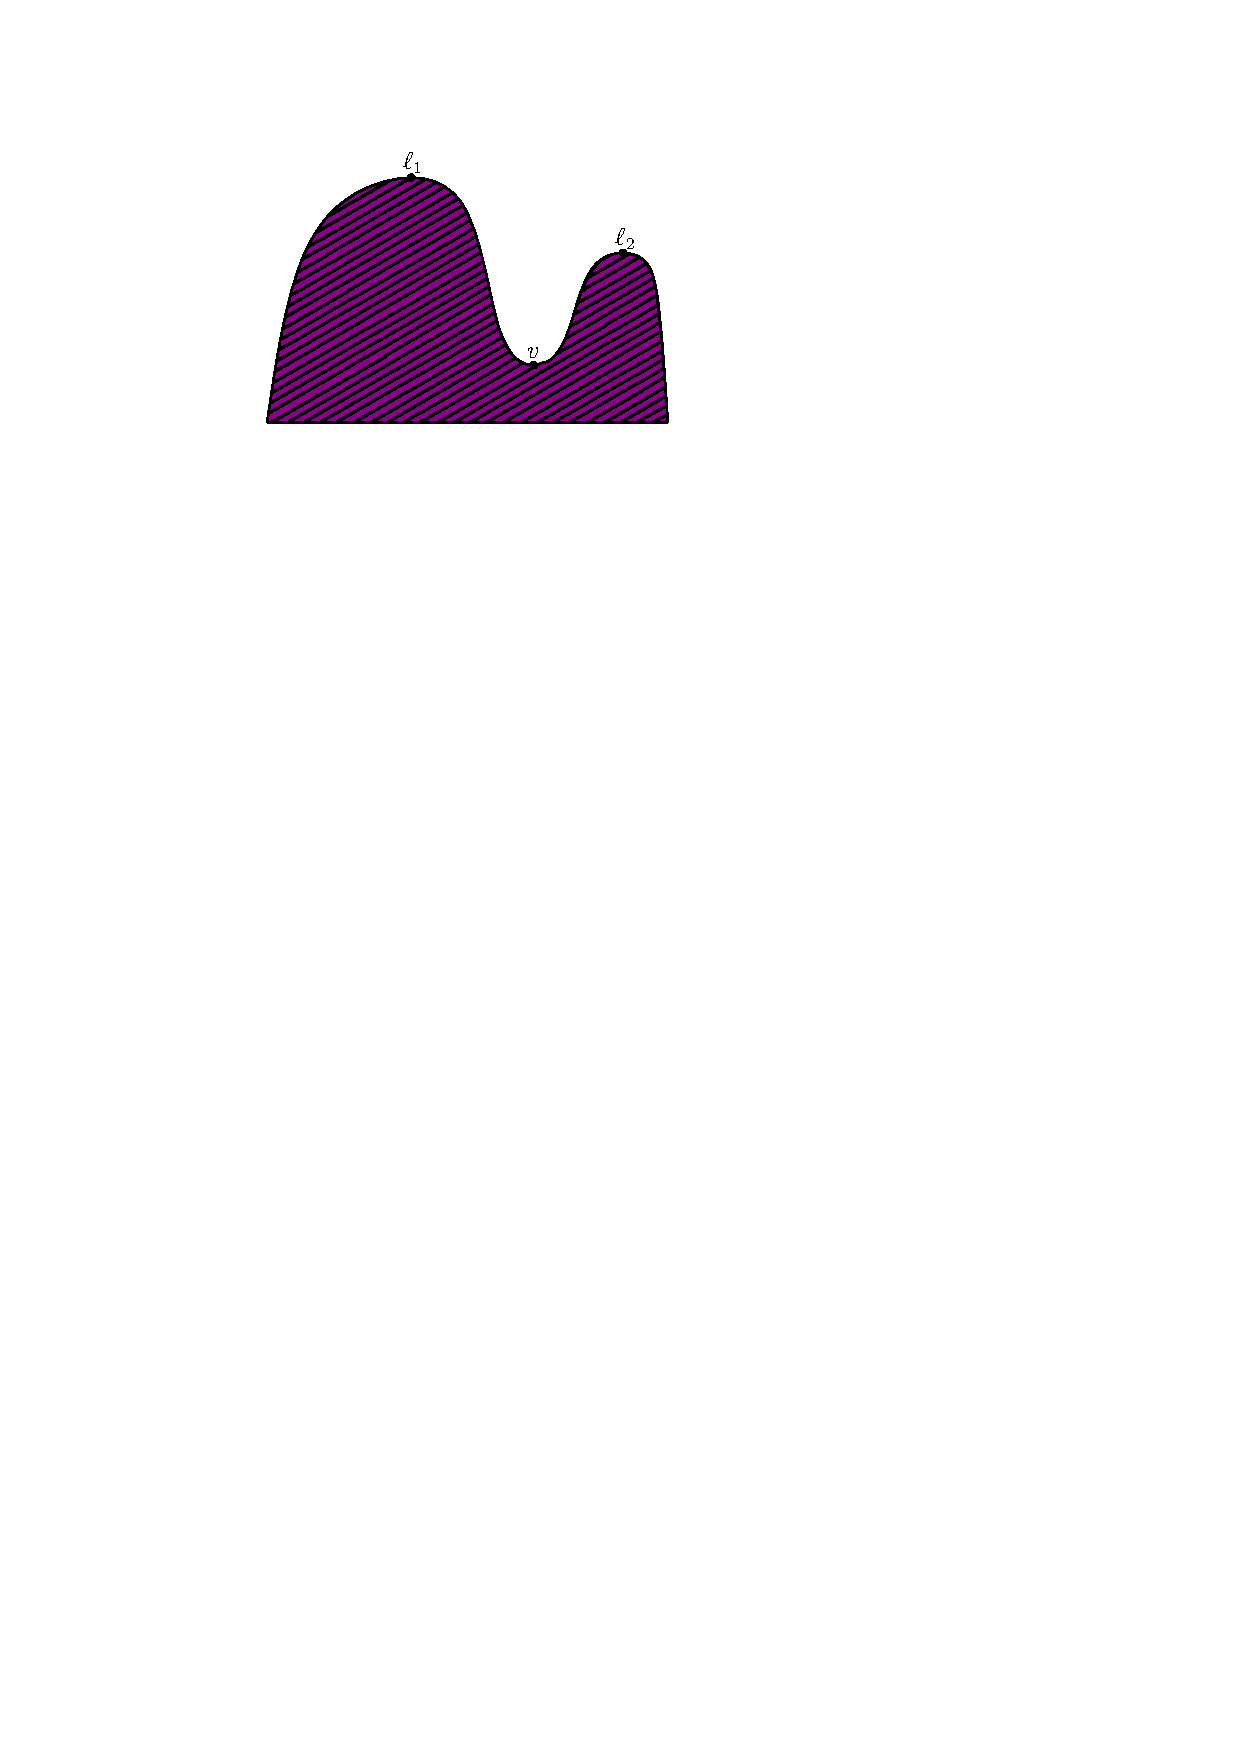
\includegraphics[width=.25\linewidth]{figs/redBlue2}%
    \hspace{.07in}
    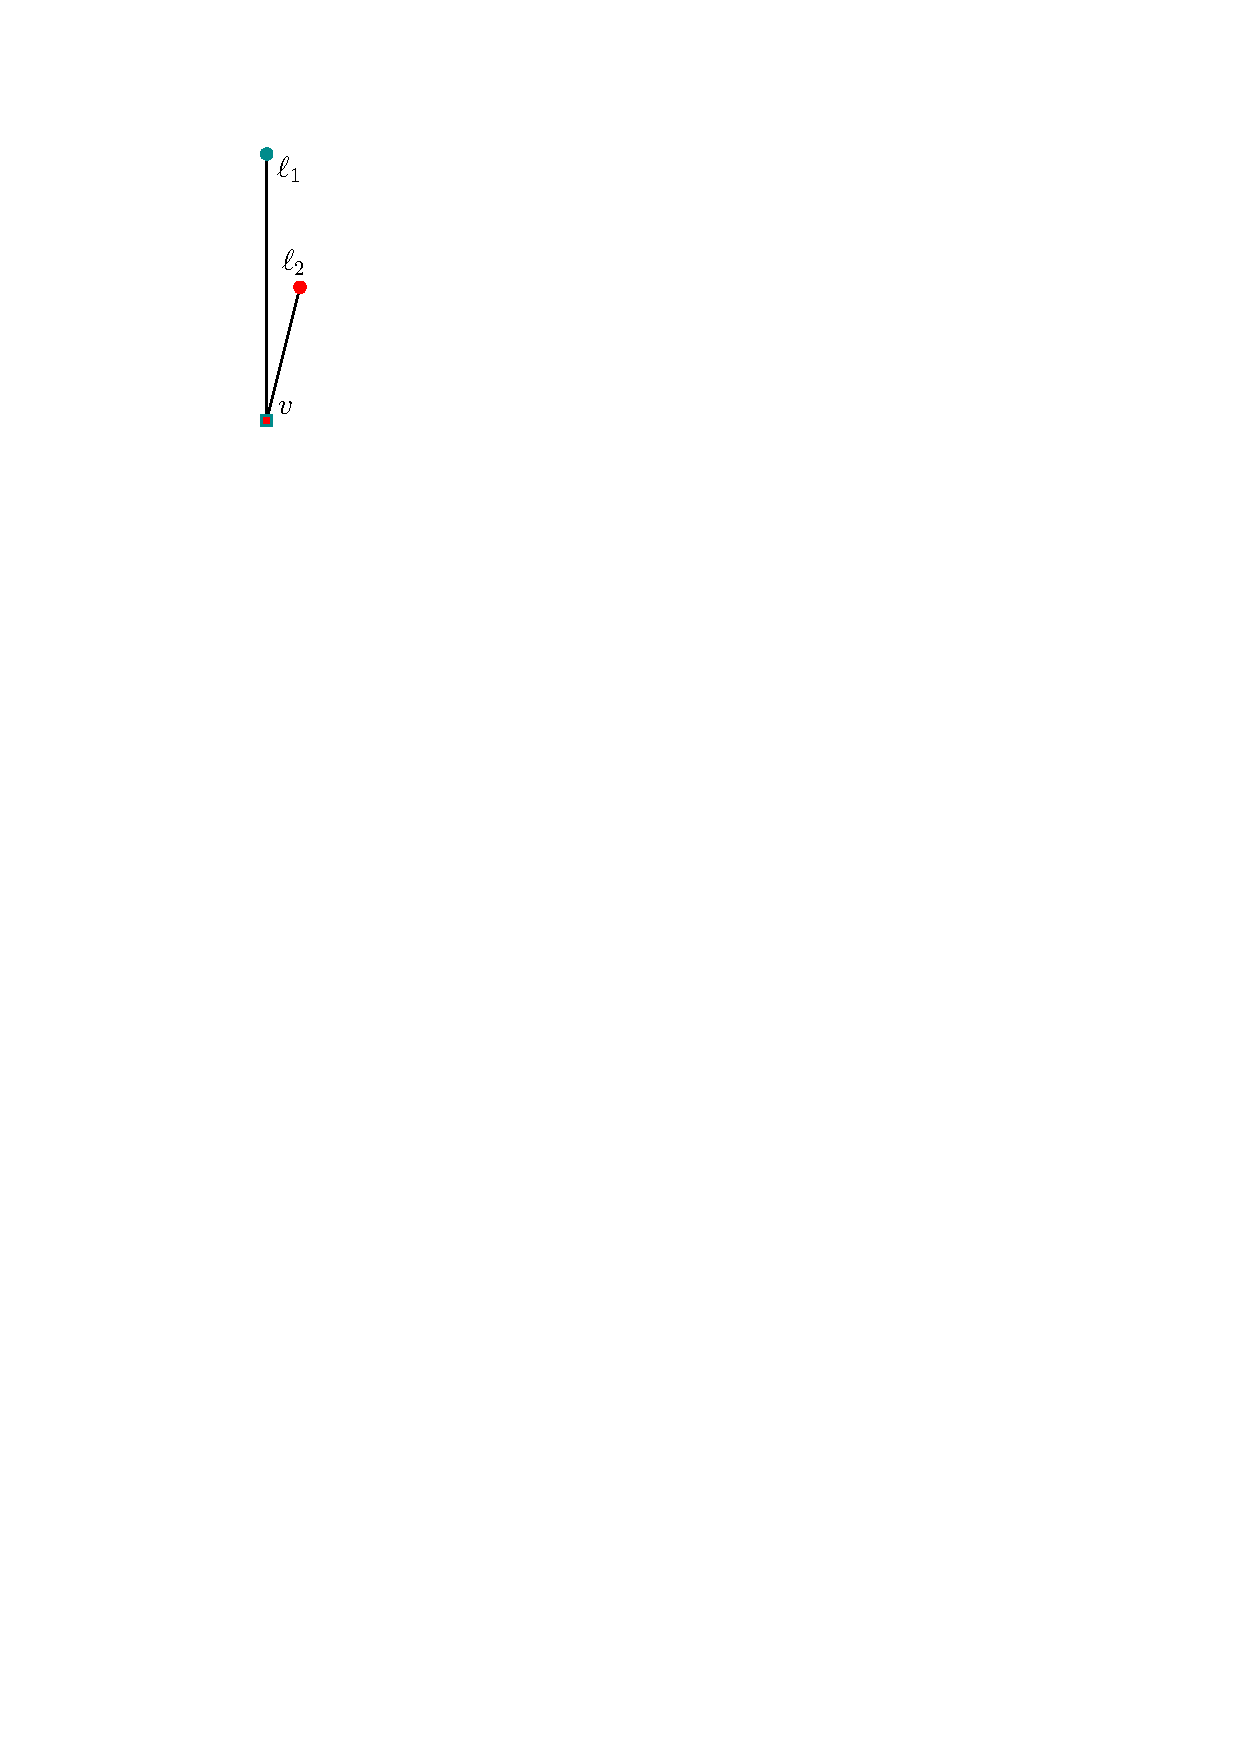
\includegraphics[width=.03\linewidth]{figs/redBlueTree}
    \hspace{.09in}
    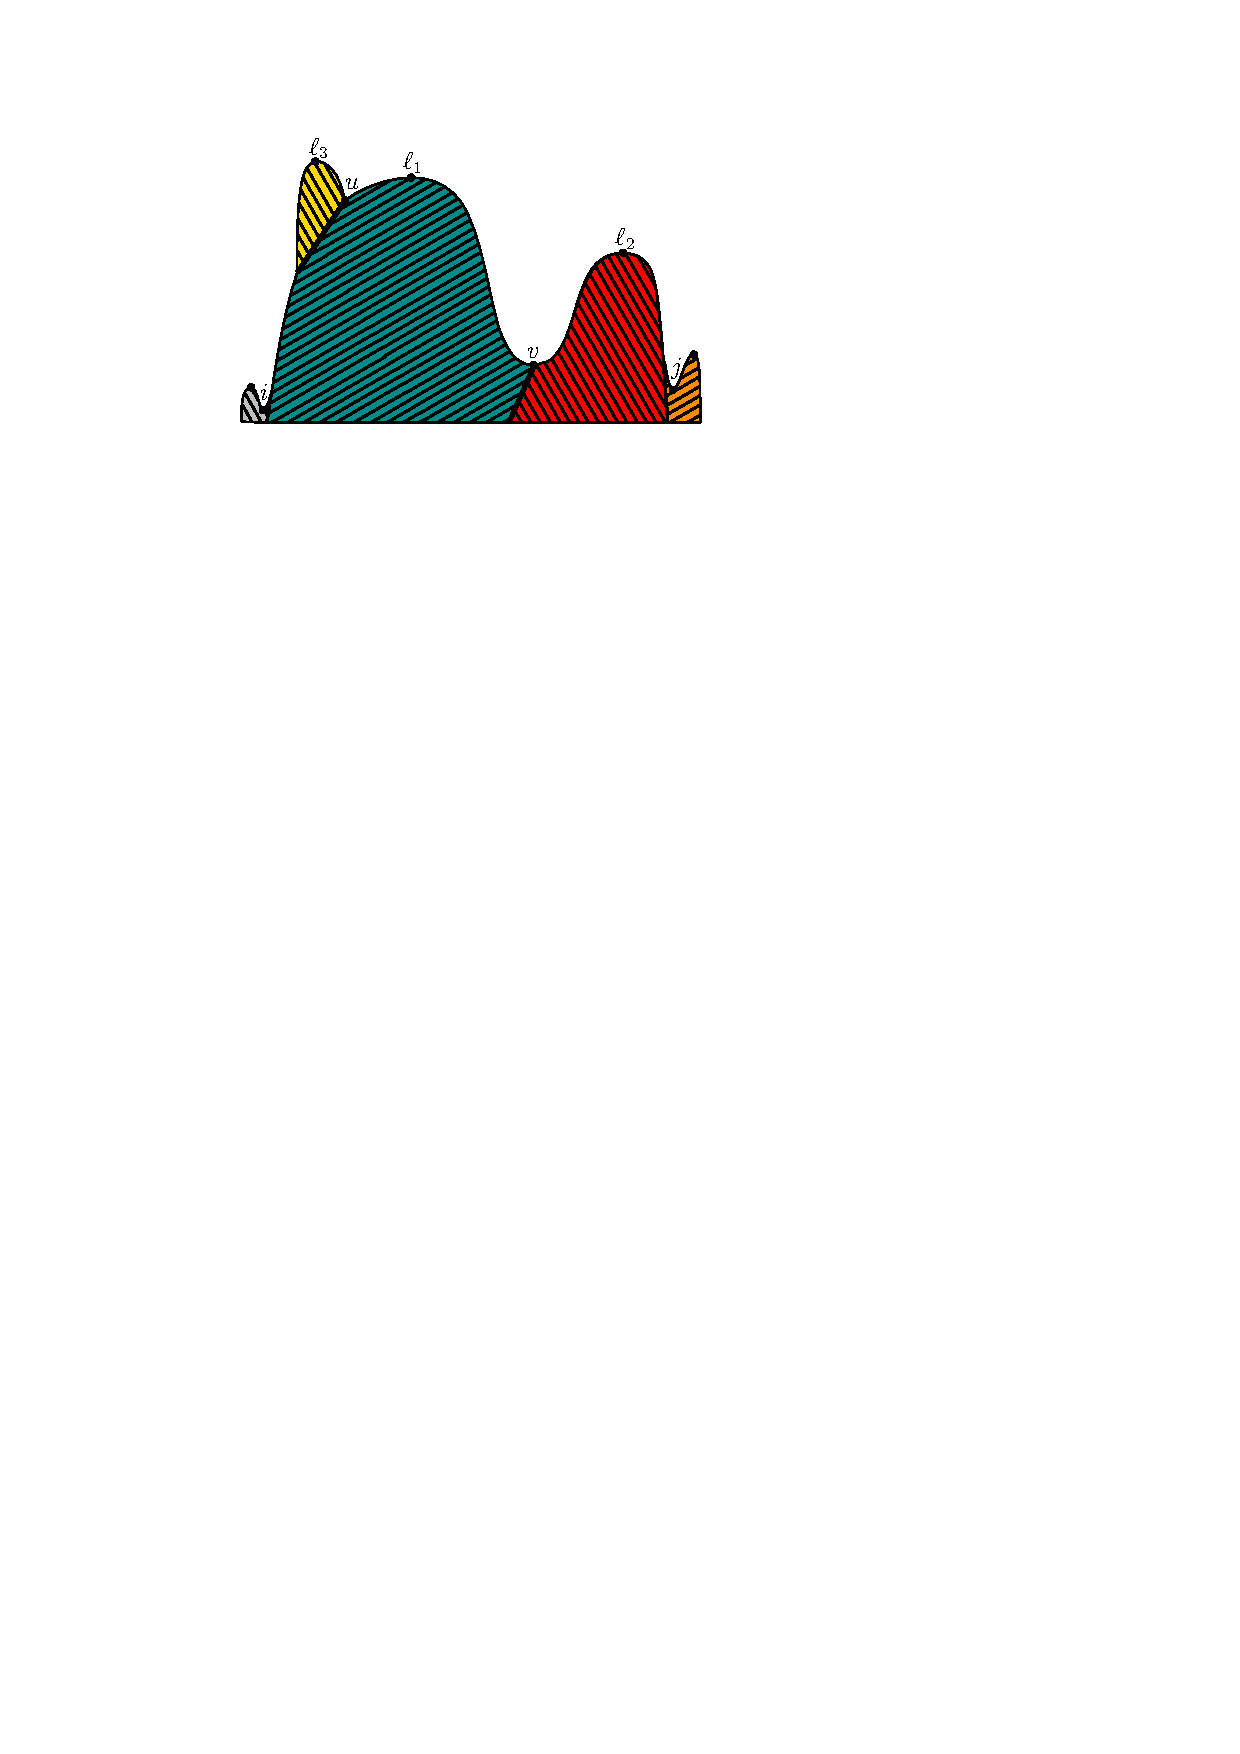
\includegraphics[width=.3\linewidth]{figs/mound}%
    \hspace{.07in}
    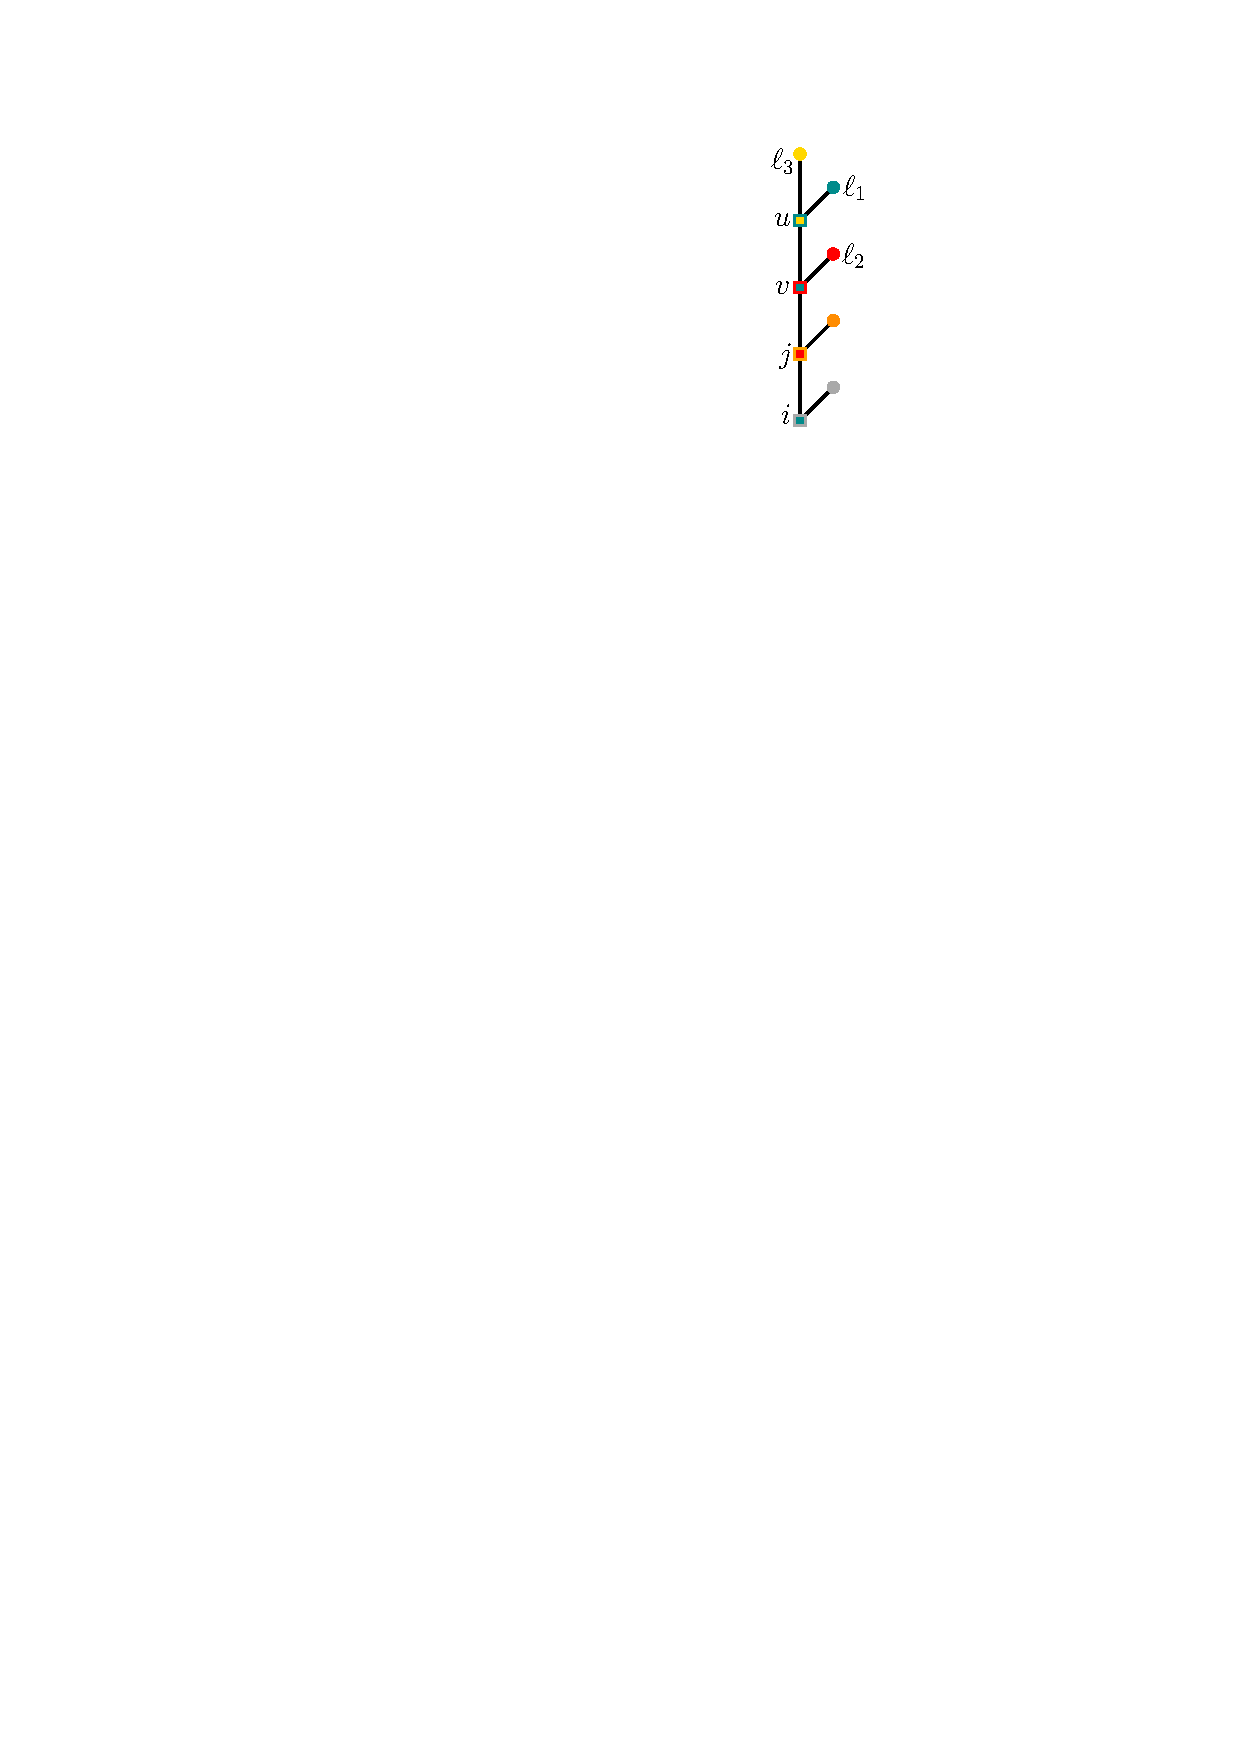
\includegraphics[width=.065\linewidth]{figs/moundTree}
    \caption{On the left, red and blue merge to make purple, followed by the contour tree with initial colors.  On the right, additional maxima and the resulting contour tree.}
    \label{fig:colors}
\end{figure}


What happens when finally blue and red join at $v$? We merge the two colors, but now have
blue and red queues of critical vertices. We also need to merge the priority queues
to get a consistent painting. And that decides the use of \emph{binomial heaps}~\cite{Vu78} to store the
critical points of one color. Merges can be done in logarithmic time, the same time
required for deletes. We stress that the feasibility of the entire approach hinges on the use of binomial heaps.

In this discussion, we ignored an annoying problem. Vertices
may actually be touched by numerous colors, not just one or two as assumed above. A simple solution
would be to insert vertices into heaps corresponding to all colors touching it. But there could
be super-constant numbers of copies of a vertex, and handling all these copies would lead
to extra overhead. We show that it suffices to simply put each vertex $v$ into at most two heaps, one for each
``side" of a possible join. We are guaranteed that when $v$ needs to be processed, all edges have
at most $2$ colors, because of all the color merges that previously occured.


\paragraph{The running time analysis:} Relating the running time to a path decomposition is the most technical part of the paper. 
All the non-heap operations can be easily bounded by $O(t\alpha(t) + N)$ (the $t\alpha(t)$ is from the union-find data structure
for colors). It is not hard to argue that at all times, any heap always contains a subset of a leaf
to root path. Unfortunately, this subset is \emph{not} contiguous, as the right part of \Fig{colors} shows. 
Specifically, in this figure the far left saddle (labeled $i$) is hit by blue paint.  However, there is another 
saddle on the far right (labeled $j$) which is not hit by blue paint.  Since this far right saddle is slightly 
higher than the far left one, it will merge into the component containing the blue mound (and also the yellow and red mounds)
before the far left one.  Hence, the vertices initially touched by blue are not contiguous in the contour tree.

Nonetheless, we can get a non-trivial (but non-optimal) bound. Let $d_v$ denote the distance to the root for vertex $v$ in the join tree.
The total cost (of the heap operations) is at most $\sum_v \log d_v$. This immediately proves a bound of $O(t\log D)$, where
$D$ is the maximum distance to the root, an improvement over previous work. But this bound is non-optimal.
For a balanced binary tree, this bound is $O(t\log\log t)$, whereas the cost of any path decomposition is $O(t)$.

The cost of heap operations depends on the sizes of the heaps, which keeps changing because
of the repeated merging. This is a major headache for the analysis. There are situations where
the initial heap sizes are small, but they eventually merge to create larger heaps. 
We employ a variant
of \emph{heavy path decompositions}, first used by Sleator and Tarjan for analyzing link/cut trees~\cite{st-dsdt-83}.
The final analysis basically charges expensive heap operations to long paths in the decomposition.

\subsection{The lower bound} 

Consider a contour tree $T$ and the path decomposition $P(T)$ used to bound the running time. 
Denoting $\cost(P(T)) = \sum_{p \in P(T)} |p|\log |p|$, we construct a set of $\prod_{p \in P(T)} |p|!$
functions on a fixed domain such that each function has a distinct (labeled) contour tree. By a simple
entropy argument, any algebraic decision tree that correctly computes the contour tree on all instances
requires worst case $\Omega(\cost(P(T)))$ time. We prove that our algorithm makes $\Theta(\cost(P(T)))$ 
comparisons on all these instances. In general, any algorithm requires $\Omega(C)$ time
to solve the set of instances that our algorithm solves with $C$ comparisons.

We have a fairly simple construction that works for terrains. In $P(T)$, consider the path
$p$ that involves the root. The base of the construction is a conical ``tent", and there
will be $|p|$ triangular faces that will each have a saddle. The heights of these saddles
can be varied arbitrarily, and that will give $|p|!$ different choices. Each of these saddles
will be connected to a recursive construction involving other paths in $P(T)$. Effectively,
one can think of tiny tents that are sticking out of each face of the main tent. The contour
trees of these tiny tents attach to a main branch of length $|p|$. Working out the details,
we get $\prod_{p \in P(T)} |p|!$ terrains each with a distinct contour tree. It is possible to argue
that our algorithm requires $\Theta(\cost(P(T)))$ comparisons on all these instances.



\FullVer{
\section{Divide and conquer through contour surgery} \label{sec:surgery}

{\bf The cutting operation:} We define a ``cut" operation on $f:\MM \rightarrow \RR$ that cuts along a regular contour to create
a new simplicial complex with an added boundary. Given contour $\phi$, this is constructing the simplicial complex $\MM \setminus \phi$. 
We will always enforce the condition that $\phi$ never passes through a vertex of $\MM$.
Again, we use $\eps$ for an infinitesimally small value. We denote $\phi^+$ (resp. $\phi^-$) to be
the contour at value $f(\phi) + \eps$ (resp. $f(\phi) - \eps$), which is at distance $\eps$
from $\phi$. 

An $h$-contour is achieved by intersecting $\MM$ with the hyperplane $x_{d+1} = h$ and taking a connected component. (Think of the $d+1$-dimension
as height.) Given some point $x$
on an $h$-contour $\phi$ (with some simplex that $x$ is present in), we can walk along $\MM$ from $x$ and determine $\phi$.
We can ``cut" along $\phi$ to get a new (possibly) disconnected simplicial complex $\MM'$. This is achieved
by splitting every facet $F$ that $\phi$ intersects into an ``upper" facet and ``lower" facet. Algorithmically,
we cut facet $F$ with $\phi^+$ and take everything above $\phi^+$ in $F$ to make the upper facet. Analogously, we cut with $\phi^-$ to get the lower facet.
The facets are then triangulated to ensure that they are all simplices.
Given that $\phi$ cannot cut a boundary and all non-boundary facets
have constant size, we omit the algorithmic description for this process. We only note that this
creates the two new boundaries $\phi^+$ and $\phi^-$, and we maintain the property of constant $f$-value at a boundary.
This new simplicial complex is denoted by $\cut(\phi,\MM)$.
This can be constructed in time linear in $|\phi|$.

%We denote this new manifold by $\cut(\phi,\MM)$, and the new boundaries by $\phi^+$ and $\phi^-$.
%Abusing notation, we use $\cut(\phi,\MM)$
%for a set $\Psi$ of contours to mean the manifold obtained by cutting along all contours in $\Phi$.


We now describe a high-level approach to construct $\reeb(\MM)$.

\medskip
\fbox{
\begin{minipage}{0.9\textwidth}
{\bf $\surgery(\MM,\phi)$}

\smallskip
\begin{asparaenum}
	\item Let $\MM' = \cut(\MM,\phi)$.
	\item Construct $\reeb(\MM')$ and let $A, B$ be the nodes corresponding to the new boundaries created
	in $\MM'$. (One is a minima and the other is maxima.)
	\item Since $A, B$ are leaves, they each have unique neighbors $A'$ and $B'$, respectively. Insert
	edge $(A',B')$ and delete $A, B$ to obtain $\reeb(\MM)$.
\end{asparaenum}
\end{minipage}}

\medskip
\begin{theorem} \label{thm:surgery} For any regular contour $\phi$, the output of $\surgery(\MM,\phi)$ is $\reeb(\MM)$.
\end{theorem}

We require some theorems from \cite{c-tmi-04} (Theorems 6.6 and 6.7) that map paths in $\cC(\MM)$ to $\MM$.

\begin{theorem} \label{thm:carr-path} For every path $P$ in $\MM$, there exists a path $Q$ in the contour tree corresponding
to the contours passing through points in $P$.
For every path $Q$ in the contour tree, there exists at least one path $P$ in $\MM$ through points present
in contours involving $Q$.
\end{theorem}

\begin{theorem} \label{thm:carr-mono} For every monotone path $P$ in $\MM$, there exists a monotone path $Q$ in the contour tree to which $P$
maps (as in the previous theorem), and vice versa.
\end{theorem}


The main theorem is a direct consequence of the following lemma. 

\begin{lemma} \label{lem:cut} Consider a regular contour $\phi$ contained in a contour class (of an edge of $\reeb(\MM))$
$(u,v)$ and denote $\MM' = \cut(\MM,\phi)$. Then $\cV(\reeb(\MM')) = \{\phi^+,\phi^-\} \cup \cV(\MM)$
and $\cE(\reeb(\MM')) = \{(u,\phi^+),(\phi^-,v)\} \cup (\cE(\MM) \setminus (u,v))$.
\end{lemma}

\begin{proof} The contours of $\MM'$ are exactly the contours of $\MM$ with $\phi^+$ and $\phi^-$, without $\phi$.
All new vertices created in $\MM'$ are present on $\phi^+$ and $\phi^-$. That proves the first part.

Any contour class in $\MM'$ (edge in $\cC(\MM')$) that does not involve $\phi^+$ or $\phi^-$ is also
a contour class in $\MM$. Furthermore, a maximal contour class satisfying these properties is also
maximal in $\MM$. So all edges of $\cC(\MM')$ that do not involve $\phi^+$ or $\phi^-$ are edges of $\cC(\MM)$.
Analogously, every edge of $\cC(\MM)$ not involving $\phi$ is an edge of $\cC(\MM')$.

Consider the contour class corresponding to edge $(u,v)$ of $\cC(\MM)$. There is a natural ordering
of the contours by function value, ranging from $f(u)$ to $f(v)$. All contours in this class ``above" $\phi$
form a maximal contour class in $\MM'$, represented by edge $(u,\phi^+)$. Analogously, there is another
contour class represented by edge $(\phi^-,v)$. We have now accounted for all contours in $\cC(\MM')$,
completing the proof.
\end{proof}

A useful corollary of this lemma shows that a contour actually splits the simplicial complex into
two disconnected complexes.

\begin{theorem} \label{thm:jordan} $\cut(\MM,\phi)$ consists of two
disconnected simplicial complexes.
\end{theorem}

\begin{proof} Denote (as in \Lem{cut}) the edge containing $\phi$ to be $(u,v)$. Suppose for contradiction that there is a path between vertices $u$ and $v$
in $\MM' = \cut(\MM,\phi)$. By \Thm{carr-path}, there is a path in $\cC(\MM')$ between $u$ and $v$. Since $\phi^+$ and $\phi^-$
are leaves in $\cC(\MM')$, this path obviously cannot use edges incident to them. By \Lem{cut},
all the edges of this path are in $\cE(\cC(\MM)) \setminus (u,v)$. So we get a cycle in $\cC(\MM)$, a contradiction.
To show that there are exactly two connected components in $\cut(\MM,\phi)$, it suffices
to see that $\cC(\MM')$ has two connected components (by \Lem{cut}) and apply \Thm{carr-path}.
\end{proof}

\section{Raining to partition $\MM$} \label{sec:rain}

In this section, we describe a linear time procedure that partitions $\MM$ into special
\emph{extremum dominant} simplicial complexes.

\begin{definition} \label{def:dom} A simplicial complex is \emph{minimum dominant} if there exists
a minimum $x$ such that every non-minimal \emph{vertex} in the manifold has a decreasing path to $x$.
Analogously define \emph{maximum dominant}. 
\end{definition}

The first aspect of the partitioning is ``raining". Start at some point $x \in \MM$ and imagine rain at $x$.
The water will flow downwards along descending paths and ``wet" all the points encountered. Note that this procedure considers all points
of the manifold, not just vertices.

\begin{definition} \label{def:wet} Fix $\MM$ and $x \in \MM$. The set of points $y \in \MM$ such that there is a non-ascending path from $x$ to $y$
is denoted by $\wet(x,\MM)$ (which is in turn is represented as a simplicial complex). A point $z$ is at the \emph{interface} of $\wet(x,\MM)$ if every neighborhood of $z$
has non-trivial intersection with $\wet(x,\MM)$.
\end{definition}

The following claim gives a description of the interface. While its meaning is quite intuitive, the proof is tedious.

\begin{claim} \label{clm:inter} For any $x$, the interface of $\wet(x,\MM)$ is a set of contours,
each containing a join vertex.
\end{claim}

\begin{proof} If $p \in \wet(x,\MM)$, all the points in any contour containing $p$ are also in $\wet(x,\MM)$.
 (Follow the non-ascending path to from $x$ to $p$ and then walk along the contour.) The converse is also true,
 so $\wet(x,\MM)$ contains entire contours.

Let $\eps, \delta$ be sufficiently small as usual. Fix some $y$ at the interface.
Note that $y \in \wet(x,\MM)$. (Otherwise, $B_\eps(y)$ is dry.)
The points in $B_\eps(y)$ that lie below $y$ have a descending path from $y$ and hence must be wet.
There must also be a dry point in $B_\eps(y)$ that is above $y$, and hence,
there exists a dry, regular $(f(y)+\delta)$-contour $\phi$ intersecting $B_\eps(y)$.

Let $\Gamma_y$ be the contour containing $y$.  Suppose for contradiction
that $\forall p \in \Gamma_y$, $p$ has up-degree $1$ (see \Def{deg}). Consider the non-ascending path from $x$ to $y$ and let $z$
be the first point of $\Gamma_y$ encountered. There exists a wet, regular $(f(y) + \delta)$-contour $\psi$ 
intersecting $B_\eps(z)$. Now, walk from $z$ to $y$ along $\Gamma_y$. If all points $w$ in this walk
have up-degree $1$, then $\psi$ is the unique $f(y)+\delta$-contour
intersecting $B_\eps(w)$. This would imply that $\phi = \psi$, contradicting the fact that $\psi$ is wet
and $\phi$ is dry.

Therefore, there must exist a join vertex $w$ in $\Gamma_y$, such that $B_\eps(w)$ intersects
both $\phi$ and $\psi$. As $\delta, \eps \rightarrow 0^+$, the limit of $\phi$ (which is dry)
lies in $\Gamma_y$ (which is wet). 
Hence this limit gives a contour of the interface containing the join $w$.
\end{proof}

Note that $\wet(x,\MM)$ (and its interface) can be computed in time linear in the size of the wet simplicial complex.
We perform a non-ascending search from $x$. Any facet $F$ of $\MM$ encountered is partially (if not entirely) in $\wet(x,\MM)$.
This portion is determined by cutting $F$ along the interface. Since the interface is a contour, this is equivalent
to cutting $F$ by a hyperplane. All these operations can be performed to output $\wet(x,\MM)$ in time linear in $|\wet(x,\MM)|$.


We define a simple \lift{} operation on the interface contours. Consider such a contour $\phi$ containing
a join vertex $y$. Take any dry increasing edge incident to $y$, and pick the point $z$ on this edge at height
$f(y) + \delta$. Let $\lift(\phi)$ be the unique contour through the regular point $z$. Note that $\lift(\phi)$ is dry.

\begin{claim} \label{clm:cut-int} Let $\phi$ be an interface contour. Then $\cut(\MM,\lift(\phi))$
results in two disjoint simplicial complexes, one consisting entirely of dry points.
\end{claim}

\begin{proof} By \Thm{jordan}, $\cut(\MM,\lift(\phi))$ results in two disjoint simplicial complexes. Let $\NN$ be the complex containing
the point $x$ (the argument in $\wet(x,\MM)$), and let $\NN'$ be the other complex. 
Any path from $x$ to $\NN'$ must intersect $\lift(\phi)$, which is dry. Hence $\NN'$ is dry.
%
%
%If there exists a wet point $z$ in $\NN'$, then there exists a descending path from $x$ to $z$. 
%As $x$ is in $\NN$ and $z$ is in $\NN'$, again by the Jordan Curve Theorem this path must intersect $\phi$, 
%contradicting the fact that $\phi$ is dry.
\end{proof}



We describe the main partitioning procedure that cuts a simplicial complex $\NN$ into extremum
dominant complexes. It takes an additional input of a maximum $x$. To initialize,
we begin with $\NN$ set to $\MM$ and $x$ as an arbitrary maximum. One of the critical aspects
of the procedure is that the rain alternately flows downwards and upwards, 
since otherwise faces may be cut a super constant number of times (see \Fig{order}).
In other words, when
we start, rain flows downwards. In each recursive call, the direction of rain is switched to the 
opposite direction. While one can implement $\rain$ this way, it is conceptually easier
to think of \emph{inverting} a complex $\NN'$ when a recursive call is made. Inversion
is easily achieved by just negating the height values. (From a running time standpoint, it suffices
to maintain a single bit associated with $\NN'$ that determines whether heights are inverted or not.)
We can now let rain flow downwards, as it usually does in our world.

%
%We critically perform
%an \emph{inversion} step, which is simply achieved by negating
%
\medskip
\fbox{
\begin{minipage}{0.9\textwidth}
{\bf $\rain(x,\NN)$}

\smallskip
\begin{compactenum}
	\item Determine interface of $\wet(x,\NN)$. 
	\item If the interface is empty, simply output $\NN$. Otherwise, denote the contours by $\phi_1, \phi_2, \ldots, \phi_k$ and set $\phi'_i = \lift(\phi_i)$.
	\item Initialize $\NN_1 = \NN$.
	\item For $i$ from $1$ to $k$: 
	\begin{compactenum}
		\item Construct $\cut(\NN_i,\phi'_i)$, consisting of dry complex $\LL_i$ and remainder $\NN_{i+1}$.
		\item Let the newly created boundary of $\LL_i$ be $B_i$. Invert $\LL_i$ so that $B_i$ is a maximum. Recursively
		call $\rain(B_i,\LL_i)$.
	\end{compactenum}
	\item Output $\NN_{k+1}$ together with any complexes output by recursive calls.
\end{compactenum}
\end{minipage}}

\medskip
For convenience, denote the total output of $\rain(x,\MM)$ by $\MM_1, \MM_2, \ldots, \MM_r$.
We first argue the correctness of $\rain$.

\begin{lemma} \label{lem:rain-1} Each output $\MM_i$ is extremum dominant.
\end{lemma}

\begin{proof} Consider a call to $\rain(x,\NN)$. If the interface is empty, then all of $\NN$
is in $\wet(x,\NN)$, so $\NN$ is trivially extremum dominant. So suppose the interface
is non-empty and consists of $\phi_1, \phi_2, \ldots, \phi_k$ (as denoted in the procedure).
By repeated applications of \Clm{cut-int}, $\NN_{k+1}$ contains $\wet(x,\MM)$. 
Consider $\wet(x,\NN_{k+1})$. The interface must exactly be $\phi_1, \phi_2, \ldots, \phi_k$.
So the only dry vertices are those in the boundaries $B_1, B_2, \ldots, B_k$. But these
boundaries are maxima.
\end{proof}

Focus on $\rain(x,\MM)$. As $\rain$ proceeds, new facets/simplices are created because of repeated cutting. Indeed, any facet $F$
in any simplicial complex $\NN$ that is recursively invoked, is achieved by cutting facet $F'$ in $\MM$.
The key to the running time of $\rain(x,\MM)$ is bounding the number of newly created facets, for which we have the following lemma.

\begin{lemma}\label{lem:new-verts}
A facet $F \in \MM$ is cut at most once during $\rain(x,\MM)$.
\end{lemma}
\begin{proof} All notation here follows that in the pseudocode of $\rain$.
First, by \Thm{jordan}, all the pieces on which $\rain$ is invoked are disjoint.
Second, all recursive calls are made on dry complexes.

Consider the first time that $F$ is cut, say, during the call to $\rain(x,\NN)$.
Specifically, say this happens when $\cut(\NN_i,\phi'_i)$ is constructed. 
So $F$ is cut by some hyperplane into lower and upper portions (which are then triangulated).
Since the cut is infinitesimally above an interface, the lower portion is basically wet.
It can never be part of $\LL_1, \LL_2, \ldots$, which go into recursive calls. This portion
is in $\NN_{k+1}$. The upper portion/facet (call it $U$) is in $\LL_i$. Note that the lower
boundary of $U$ is in the boundary $B_i$. Since a recursive call is made to $\rain(B_i,\LL_i)$
(and $\LL_i$ is inverted), $U$ becomes wet. Hence, $U$ will not be cut subsequently.
All in all, $F$ is cut at most once.
\ignore{
As the number of edges is $O(n)$, arguing that there is at most one boundary vertex created along any given edge will imply the claim.
Consider some edge $e$ and take the first time a boundary vertex is created in $e$.
This happens when some contour $\phi$ intersects $e$. On applying $\cut(\NN,\lift(\phi))$,
consider the dry manifold $\LL$ and wet manifold $\MM$ constructed. The edge $e$ is split into two parts, the dry and wet part.
The wet part is in $\MM$ and will never be involved in any recursive call.

The dry part of $e$ (call it $e'$) needs to be considered.
A boundary vertex $v$ (an new endpoint of $e$) is created, which is part of the boundary $B$ in $\LL$,
such that $\rain(B,\LL)$ is called to the inverted $\LL$. In this call, since the water starts from $v$,
all of $e'$ becomes wet. So there is no further interface contour that can intersect this portion of $e'$.
}
\end{proof}


\begin{theorem} \label{thm:rain-time} The total running time of $\rain(x,\MM)$ is $O(|\MM|)$.
\end{theorem}

\begin{proof} The operations performed are the raining and cutting. We can bound this by the total
complexities of the wet complexes and the new boundaries created. No facet is ever wet twice,
and by \Lem{new-verts}, the total number of facets that every appear is $O(|\MM|)$. This also 
bounds the complexities of the boundaries created.
\end{proof}



\begin{claim} \label{clm:rain-reeb} Given $\reeb(\MM_1), \reeb(\MM_2), \ldots, \reeb(\MM_r)$, 
%be the output of $\rain(x,\MM)$. Suppose that for each reeb graph we know its corresponding vertex in the Manifold Ordering Tree. 
$\reeb(\MM)$ can be constructed in $O(|\MM|)$ time.
\end{claim}

\begin{proof} Consider the tree of recursive calls in $\rain(x,\MM)$, with each node
labeled with some $\MM_i$.
Walk through this tree in a leaf first ordering.  Each time we visit a node we connect its contour tree to the 
contour tree of its children in the tree using the $\surgery$ procedure. 
Each $\surgery$ call is constant time, and the total time is the size of the recursion tree.
\end{proof}


\section{Contour trees of extremum dominant manifolds} \label{sec:extreme}

The previous section allows us to restrict attention to extremum dominant manifolds.
We will orient so that the extremum in question is always a \emph{minimum}.
We will fix such a simplicial complex $\MM$, with the dominant minimum $m^*$. 
The set of non-dominant minima is denoted by $M$.
For vertex $v$, we use $\MM^+_v$ to denote the simplicial complex obtained by only
keeping vertices $u$ such that $f(u) > f(v)$. Analogously, define $\MM^-_v$. Note that $\MM^+_v$ may contain
numerous connected components. 

The main theorem of this section asserts that the contours trees of minimum dominant manifolds have a simple description.
The exact statement will require some definitions and notation.
We required the notions of \emph{join} and \emph{split} trees, as given by~\cite{csa-cctad-00}.
Conventially, all edges are directed from higher to lower function value. 

\begin{definition} \label{join} The join tree $\cJ(\MM)$ of $\MM$ is built on vertex set $V(\MM)$.
The directed edge $(u,v)$ is present when $u$ is the smallest valued vertex in a connected component of $\MM^+_v$
\emph{and} $v$ is connected to this component (in $\MM$). The split tree $\cS(\MM)$ is obtained
by looking at $\MM^-_v$ (or alternately, by taking the join tree of the inversion of $\MM$). 
\end{definition}


Some basic facts about these trees. 
%Note that unlike the contour tree, all vertices in $\MM$ are present in $\cJ(\MM)$ and $\cS(\MM)$. 
All outdegrees in $\cJ(\MM)$ are at most $1$, all indegree $2$ vertices are joins, all leaves are maxima,
and the global minimum is the root. All indegrees in $\cS(\MM)$ are at most $1$, all outdegree $2$
vertices are splits, leaves are minima, and the global maximum is the root.
%
As these trees rooted, we can use ancestor-descendant terminology.  
Specifically, for two adjacent vertices $u$ and $v$, $u$ is the parent of $v$ if $u$ is closer to the root 
(i.e. each node can have at most one parent, but can have two children).  


The key observation is that $\cS(\MM)$ is trivial for a minimum dominant $\MM$.



\begin{lemma} \label{lem:split} $\cS(\MM)$ consists of:
\begin{asparaitem}
	\item A single path (in sorted order) with all vertices except non-dominant minima.
	\item Each non-dominant minimum is attached to a unique split (which is adjacent to it).
\end{asparaitem}
\end{lemma}

\begin{proof} It suffices to prove that each split $v$ has one child that is just a leaf, which
is a non-dominant minimum.  Specifically, any minimum is a leaf in $\cS(\MM)$ and thereby attached to a split, 
which implies that if we removed all non-dominant minima, we must end up with a path, as asserted above.

Consider a split $v$. For sufficiently small $\eps, \delta$, there are exactly two $(f(v) - \delta)$-contours
$\phi$ and $\psi$ intersecting $B_\eps(v)$. Both of these are regular contours. There must be a non-ascending
path from $v$ to the dominant minimum $m^*$. Consider the first edge (necessarily decreasing from $v$)
on this path. It must intersect one of the $(f(v) - \delta)$-contours, say $\phi$. By \Thm{jordan}, $\cut(\MM,\phi)$ has
two connected components, with one (call it $\LL$) having $\phi^-$ as a boundary maximum. This complex
contains $m^*$ as the non-ascending path intersects $\phi$ only once. Let the other
component be called $\MM'$.

Consider $\cut(\MM',\psi)$ with connected component $\NN$ having $\psi^-$ as a boundary. $\NN$
does not contain $m^*$, so any path from the interior of $\NN$ to $m^*$ must intersect the boundary $\psi^-$.
But the latter is a maximum in $\NN$, so there can be no non-ascending path from the interior to $m^*$.
Since $\MM$ is overall minimum dominant, the interior of $\NN$ can only contain a single vertex $w$, a non-dominant
minimum.

The split $v$ has two children in $\cS(\MM)$, one in $\NN$ and one in $\LL$. The child in $\NN$ can only
be the non-dominant minimum $w$, which is a leaf. 
\end{proof}

It is convenient to denote the non-dominant minima as $m_1, m_2, \ldots, m_k$
and the corresponding splits (as given by the lemma above) as $s_1, s_2, \ldots, s_k$. 

Using the above lemma we can now prove that computing the contour tree for a minimum dominant manifold 
amounts to computing its join tree.  Specifically, to prove our main theorem, we rely on the correctness of the
merging procedure from~\cite{csa-cctad-00} that constructs the contour tree from the join and split trees. 
It actually construsts the \emph{augmented contour tree} $\cA(\MM)$, which
is the contour tree with regular points inserted into the edges. 
Consider tree $T$ with vertex $v$ of in and outdegree at most $1$.
\emph{Erasing} $v$ from $T$ is the following operation: if $v$ is a leaf, just delete $v$. Otherwise, smooth $v$ out
(delete $v$ and connect its neighbors by an edge). This tree is denoted by $T \ominus v$.


\medskip
\fbox{
\begin{minipage}{0.9\textwidth}
{\bf $\merge(\cJ(\MM),\cS(\MM))$}

\smallskip
\begin{compactenum}
	\item Set $\cJ = \cJ(\MM)$ and $\cS = \cS(\MM)$.
	\item Denote $v$ as \emph{candidate} if sum of indegree of $v$ in $\cJ$ and outdegree of $v$ in $\cS$ is $1$. 
	\item Add all candidates to queue.
	\item While candidate queue is non-empty: 
	\begin{compactenum}
		\item Let $v$ be head of queue. If $v$ is leaf in $\cJ$, consider its edge in $\cJ$. Otherwise
		consider its edge in $\cS$. In either case, denote the edge by $(v,w)$.
		\item Insert $(v,w)$ in $\cA(\MM)$. 
		\item Set $\cJ = \cJ \ominus v$ and $\cS = \cS \ominus v$. Enqueue any new candidates.
	\end{compactenum}
	\item Smooth out all regular vertices in $\cA(\MM)$ to get $\cC(\MM)$.
\end{compactenum}
\end{minipage}}

\medskip

\begin{definition} 
\label{def:criticalJoin}
The critical join tree $\jc(\MM)$ is built on the set $V'$ of all
critical points other than the non-dominant minima. 
The directed edge $(u,v)$ is present when $u$ is the smallest valued vertex in $V'$ in a connected component of $\MM^+_v$
and $v$ is connected to this component (in $\MM$). 
\end{definition}


\begin{theorem} \label{thm:contour-tree} Let $\MM$ have a dominant minimum. 
The contour tree $\cC(\MM)$ consists of all edges $\{(s_i, m_i)\}$ and $\jc(\MM)$.
\end{theorem}


\begin{proof} We first show that $\cA(\MM)$ is $\cJ(\MM) \ominus \{m_i\}$ with edges $\{(s_i,m_i)\}$.
We have flexibility in choosing the order of processing in $\merge$. We first put the non-dominant
maxima $m_1, \ldots, m_k$ into the queue. As these are processed, the edges $\{(s_i,m_i)\}$ are inserted 
into $\cA(\MM)$. Once all the $m_i$'s are erased, $\cS$ becomes a path, so all outdegrees are at most $1$.
The join tree is now $\cJ(\MM) \ominus \{m_i\}$. We can now process $\cJ$ leaf by leaf, and all
edges of $\cJ$ are inserted into $\cA(\MM)$.

Note that $\cC(\MM)$ is obtained by smoothing out all regular points from $\cA(\MM)$. Smoothing out regular
points from $\cJ(\MM) \ominus \{m_i\}$ exactly yields the edges described in the theorem.
\end{proof}

\section{Painting to compute contour trees}
\label{sec:paint}

The main algorithmic contribution is a new algorithm for computing join trees of any triangulated simplicial
complex $\MM$.


{\bf Painting:} The central tool is a notion 
of \emph{painting} $\MM$. Initially associate a color with each maximum. Imagine there being a large
can of paint of a distinct color at each maxima $x$. We will spill different paint from each maximum and watch it flow down.
This is analogous to the raining in the previous section, but paint is a much more viscous liquid.
\emph{So paint only flows down edges, and it does not color the interior of facets.} Furthermore, paints
do not mix, so every edge of $\MM$ gets a unique color. This process (and indeed the entire algorithm)
works purely on the 1-skeleton of $\MM$, which is just a graph.
%

We now restate \Def{paint}.

\begin{definition} Let the 1-skeleton of $\MM$ have edge set $E$ and maxima $X$.
A  \emph{painting} of $\MM$ is a map $\chi:X \cup E \mapsto [|X|]$ with the following property. 
 Consider an edge $e$. There exists a descending path from some maximum $x$ to $e$
	consisting of edges in $E$, such that all edges along this path have the same color as $x$. 

An \emph{initial} painting has the additional property that the restriction $\chi:X \mapsto [|X|]$ is a bijection.
\end{definition}

A painting only colors edges, not vertices. We associate certain
sets of colors with vertices.

\begin{definition} \label{def:color-set} Fix a painting $\chi$ and vertex $v$.
\begin{asparaitem}
	 \item An \emph{up-star} of $v$ is the set of edges that all connected to a fixed component of $\MM^+_v$.
	 \item A vertex $v$ is \emph{touched by color $c$} if $x$ is incident to a $c$-colored
	 edge with $v$ at the lower endpoint. For $v$, $\col(v)$ is the set of colors that touch $v$.
	 \item A color $c \in \col(v)$ \emph{fully touches} $v$ if all edges in an up-star are colored $v$.
\end{asparaitem}
\end{definition}

Each non-maxima $v$ participates in at least $1$ and at most $2$ up-stars (the latter iff
$v$ is a join).


\subsection{The data structures} \label{sec:struct}

We discuss all the initializations in the next section.

\medskip
\noindent
{\bf The binomial heaps $\touch(c)$:} For each color $c$, $\touch(c)$ is a subset of vertices touched by $c$,
This is stored as a \emph{binomial max-heap} keyed by vertex heights. Abusing notation, $\touch(c)$ refers
both to the set and the data structure used to store it.


\medskip
\noindent
{\bf The union-find data structure on colors:} We will repeatedly perform unions
of classes of colors, and this will be maintained as a standard union-find data structure.
For any color $c$, $\rep(c)$ denotes the representative of its class. 

\medskip
\noindent
{\bf The stack $\st$:} This consists of non-extremal critical points, with monotonically increasing
heights as we go from the base to the head.
\ignore{
Each point $x \in \st$ has an associated subset of $\col(x)$, denoted $\mcol(x)$.
Both $\mcol(x)$ and its complement are stored as hash table. So lookups, inserts, and deletes
are in these sets are all constant time operations. The stack is guaranteed to satisfy 
the following invariants.
\begin{asparaitem}
	\item For every $x \in \st$: For every $c \in \mcol(x)$, $x$ is the highest element
	in $T(c)$. Furthermore, $c = \rep(c)$.
	\item Consider $x, y \in \st$ such that $y$ was pushed on $x$. There exists $c \in \col(x) \setminus
	\mcol(x)$ such that $x$ is not highest in $T(c)$ but $y$ is highest in $T(c)$.
\end{asparaitem}
}

\medskip
\noindent
{\bf Attachment vertex $\h(c)$:} For each color $c$, we maintain a critical point $\h(c)$ of this color.
We will maintain the guarantee that the portion of the contour tree above (and including) $\h(c)$ has already been constructed.
%This is initialized to the maximum corresponding to $c$.

	
\subsection{The algorithm} \label{sec:algo}

We formally describe the algorithm below. 
We require a technical definition of \emph{ripe} vertices.


\begin{definition} \label{def:ripe} A vertex $v$ is \emph{ripe} if: for all $c \in \col(v)$, $v$
is present in $T(\rep(c))$ and is also highest vertex in the heap. 
%Also, for all $c \in \col(v) \setminus \fcol(v)$, $T(\rep(c))$ is empty.
\end{definition} 

\medskip
\fbox{
\begin{minipage}{0.9\textwidth}
{\bf $\init(\MM)$}

\smallskip
\begin{compactenum}
	\item Construct an initial painting of $\MM$ using a descending BFS from maxima that does not explore previously colored edges.
	\item Determine all critical points in $\MM$. For each $v$, look at $(f(v) \pm \delta)$-contours in $f|_{B_\eps(v)}$ 
	to determine the up and down degrees. 
	\item Mark each critical $v$ as unprocessed.
	\item For each critical $v$ and each up-star, pick arbitrary color $c$ touching $v$. Insert $v$ into $T(c)$.
	\item Initialize $\rep(c) = c$ and set $\h(c)$ to be the unique maximum colored $c$.
\end{compactenum}
\end{minipage}}


\medskip
\fbox{
\begin{minipage}{0.9\textwidth}
{\bf $\build(\MM)$}

\smallskip
\begin{compactenum}
	\item Run $\init(\MM)$.
	\item While there are unprocessed critical points:
	\begin{compactenum}
		\item Run $\update(\st)$. Pop $\st$ to get $h$.
		\item Let $\cur(h) = \{\rep(c) | c \in \col(h)\}$.
		\item For all $c' \in \cur(h)$:
		\begin{compactenum}
			\item Add edge $(\h(c'),h)$ to $\jc(\MM)$.
			\item Delete $h$ from $T(c')$.
		\end{compactenum}
	\item Merge heaps $\{T(c') | c' \in \cur(h)\}$.
	\item Take union of $\cur(h)$ and denote resulting color by $\widehat{c}$.
	\item Set $\h(\widehat{c}) = h$ and mark $h$ as processed.
	\end{compactenum}
\end{compactenum}
\end{minipage}}

\medskip
\fbox{
\begin{minipage}{0.9\textwidth}
{\bf $\update(\st)$}

\smallskip
\begin{compactenum}
	\item If $K$ is empty, push arbitrary unprocessed critical point $v$.
	\item Let $h$ be head of $\st$.
	\item While $h$ is not ripe:
	\begin{compactenum}
		\item Find $c \in \col(h)$ such that $h$ is not the highest in $T(\rep(c))$.
		\item Push the highest of $T(\rep(c))$ onto $\st$, and update head $h$.
	\end{compactenum}
\end{compactenum}
\end{minipage}}

\bigskip

A few simple facts:
\begin{compactitem}
	\item At all times, the colors form a valid painting.
	\item Each vertex is present in at most $2$ heaps. After processing, it is removed from all heaps.
	\item After $v$ is processed, all edges incident to $v$ have the same color (technically, same representative). 
%	\item When $\update(\st)$ terminates, the head $h$ is ripe. 
	\item Vertices on the stack are in increasing height order. 
\end{compactitem}

\begin{observation}
\label{obs:twoQueues}
 Each unprocessed vertex is always in exactly one queue of the colors in each up-star.  Specifically, 
 for a given up-star of a vertex $v$, $\init(\MM)$ puts $v$ into the queue of exactly one color, say $c$.  As time goes on this queue 
 may merge with other queues, but while unprocessed $v$ is only ever (and always) in the queue of $\rep(c)$,  
 since $v$ is never added to a new queue and is not removed until it is processed.  
 In particular, finding the queues of a vertex in $\update(K)$ requires at most two union find operations (assuming each vertex records its two colors from $\init(\MM)$)
\end{observation}


\medskip
\ignore{	
	Suppose $\mcol(h) = \{c\}$ (so $h$ is split). 
	\begin{compactenum}
		\item Connect $h$ (in $\reeb(\MM)$) to $\h(c)$ and the unique minimum corresponding to split $h$. 
		\item Delete $h$ from $T(c)$, set $\h(c) = h$.
		\item End procedure.
	\end{compactenum}
	\item Let $\mcol(h) = \{c_1, c_2\}$ (so $h$ is merge).
	\item Connect $h$ in $\reeb(\MM)$ to $\h(c_1)$ and $\h(c_2)$.
	\item Delete all copies of $h$ from $T(c_1)$ and $T(c_2)$.
	\item Perform union of colors $c_1$ and $c_2$ (denote merged color as $c$). Merge heaps
	to get $T(c) = T(c_1) \cup T(c_2)$.
	\item Set $\h(c) = h$.	

We state the primary invariant below.
First, some notation. For any $v$, let $\psi^-_v$ denote the $(f(v)-\delta)$-contour intersecting
$B_\eps(v)$. If there are two such contours (so $v$ is a split), choose the one that contains
the dominant minimum. The \emph{palette} $\pal$ is the set of colors currently used,
which is $\{T(\rep(c)) | c \in |X|\}$.


Observe that $\build(\MM)$ loops over all unprocessed critical point.
The invariant is true at the starting point of each such iteration.

\medskip
\textbf{Invariant:} 
\begin{compactenum}
	\item For every $c \in \pal$, the subtree of $\cJ(\MM)$ rooted at $\h(c)$ has been constructed.
	\item Fix $c \in \pal$. Consider the set $S$ of maxima of $\MM$ in the subtree of $\cJ(\MM)$ rooted at $\h(c)$.
	Then $\rep(c) = \bigcup_{s \in S} \chi(s)$.
	\item Let $\Psi = \{\psi^-_{\h(c)} | c \in \pal\}$. The coloring given by $\rep(\cdot)$
	is a valid painting of $\cut(\MM,\Psi)$, where $\psi^-_{\h(c)}$ has color $c$.
\end{compactenum}

\medskip
It is easy to see that the invariant is true at the very beginning of the algorithm.
Each $\h(c)$ is simply the maximum colored with $c$, and we have a valid painting of $\MM$.
}


\subsection{Proving correctness} \label{sec:correct}

\ignore{
\begin{claim} \label{clm:process} Assume the invariant. Any vertex with a non-increasing path to some $\h(c)$
for $c \in \pal$ has been processed.
\end{claim}

\begin{proof} This is a direct consequence of \Thm{carr-mono}, which relates monotone paths in $\MM$ to $\cC(\MM)$.
Since the subtree of $\cJ(\MM)$ (which is basically the subtree of $\cC(\MM)$) rooted at $\h(c)$ 
has been found, all vertices in this subtree must be processed. These are all the vertices with non-increasing paths
to $\h(c)$ in $\cC(\MM)$, which by \Thm{carr-mono} is the same as those in $\cC(\MM)$.
\end{proof}
}

Our main workhorse is the following technical lemma. 

\begin{lemma} \label{lem:full} Suppose vertex $v$ is connected to a component $\PP$ of $\MM^+_v$
by edge $e$ which is currently colored $c$. Either all edges in $\PP$ are currently colored $c$, or there
exists critical vertex $w \in \PP$ fully touched by $c$ and touched by another color.
\end{lemma}

\begin{proof} Since $e$ has color $c$,
there must exist vertices in $\PP$ touched by $c$. Consider the highest
vertex $w$ in $\PP$ that is touched by $c$ and some other color. If no such vertex exists,
this means all edges incident to a vertex touched by $c$ are colored $c$. By walking through
$\PP$, we deduce that all edges are colored $c$. 

So assume $w$ exists. Take the $(f(w)+\delta)$-contour $\phi$ that intersects $B_\eps(v)$
and intersect some $c$-colored edge incident to $w$. Note that all edges intersecting $\phi$ are also colored $c$,
since $w$ is the highest vertex to be touched by $c$ and some other color. (Take the path of $c$-colored
edges from the maximum to $w$. For any point on this path, the contour passing through this point must
be colored $c$.) Hence, $c$ fully touches $w$. 
But $w$ is touched by another color, and the corresponding edge cannot intersect $\phi$. So $w$
must have up-degree $2$ and is critical.
\end{proof}

\begin{corollary}
\label{cor:terminate}
 Each time $\update(K)$ is called, it terminates with a ripe vertex on top of the stack.
\end{corollary}
\begin{proof}
 $\update(K)$ is only called if there are unprocessed vertices remaining, and so by the time we reach step 3 in 
 $\update(K)$, the stack has some unprocessed vertex $h$ on it.  
 If $h$ is ripe, then we are done, so suppose otherwise.
 
 Let $\PP$ be one of the components of $\MM^+_h$.  By construction, $h$ was put in the heap of some initial 
 adjacent color $c$.  Therefore, $h$ must be in the current heap of $\rep(c)$ (see \Obs{twoQueues}).  
 Now by \Lem{full}, either all edges in $\PP$ are colored $\rep(c)$ or  
 there is some vertex $w$ fully touched by $\rep(c)$ and some other color.  
 The former case implies that if there are any unprocessed vertices in $\PP$ then they are all in $T(\rep(c))$, 
 implying that $h$ is not the highest vertex and a new higher up unprocessed vertex will be put on the stack for the next iteration of the while loop.  
 Otherwise, all the vertices in $\PP$ have been processed.  
 However, it cannot be the case that all vertices in all components of $\MM^+_h$ have already been processed, 
 since this would imply that $h$ was ripe, and so one can apply the same argument to the other non-fully processed component. 
 
 Now consider the latter case, where we have a non-monochromatic vertex $w$.
 In this case $w$ cannot have been processed (since after being processed it is touched only by one color), 
 and so it must be in $T(\rep(c))$ since it must be in some heap of a color in each up-star (and one up-star is entirely colored $\rep(c)$).
 As $w$ lies above $h$ in $\MM$, this implies $h$ is not on the top of this heap.
\end{proof}

We prove a series of claims that will lead to the correctness proof.

\begin{claim} \label{clm:upstar} Consider a ripe vertex $v$ and take the up-star connecting
to some component of $\MM^+_v$. All edges in this component and the up-star have the same color.
\end{claim}

\begin{proof} Let $c$ be the color of some edge in this up-star.
By ripeness, $v$ is the highest in $T(\rep(c))$.
Denote the component of $\MM^+_v$ by $\PP$.
By \Lem{full}, either all edges in $\PP$ are colored $\rep(c)$ or there exists critical vertex $w \in \PP$
fully touched by $\rep(c)$ and another color. In the latter case, $w$ has not been processed,
so $w \in T(\rep(c))$ (contradiction to ripeness). Therefore, all edges in $\PP$ are colored $\rep(c)$.
\end{proof}


\begin{claim} \label{clm:process} The partial output on the processed vertices is exactly
the restriction of $\jc(\MM)$ to these vertices.
\end{claim}

\begin{proof} More generally, we prove the following: all outputs on processed vertices
are edges of $\jc(\MM)$ and for any current color $c$, $\h(c)$ is the lowest processed vertex
of that color. We prove this by induction on the processing order. The base case is is trivially
true, as initially the processed vertices and attachments of the color classes are the set of maxima.
For the induction step, consider the situation
when $v$ is being processed.

Since $v$ is being processed, we know by \Cor{terminate} that it is ripe. Take any up-star of $v$, and the corresponding component $\PP$
of $\MM^+_v$ that it connects to. By \Clm{upstar}, all edges in $\PP$ and the up-star
have the same color (say $c$). If some critical vertex in $\PP$ is not processed,
it must be in $T(c)$, which violates the ripeness of $v$.
Thus, all critical vertices in $\PP$ have been processed, and so by the induction hypothesis, the restriction of $\jc(\MM)$ to $\PP$ has been correctly computed.
Additionally, since all critical vertices in $\PP$ have processed, they all have the same color $c$ of the lowest critical vertex in $\PP$.
Thus by the strengthened induction hypothesis, this lowest critical vertex is $\h(c)$.

If there is another component of $\MM^+_v$, the same argument implies 
the lowest critical vertex in this component is $\h(c')$ (where $c'$ is the color of edges in the respective component).
Now by the definition of $\jc(\MM)$, the critical vertex $v$ connects to the lowest critical vertex in each component of $\MM^+_v$, 
and so by the above $v$ should connect to $\h(c)$ and $\h(c')$, which is precisely what $v$ is connected to by $\build(\MM)$.
Moreover, $\build$ merges the colors $c$ and $c'$ and correctly sets $v$ to be the attachment, 
as $v$ is the lowest processed vertex of this merged color (as by induction $\h(c)$ and $\h(c')$ were the lowest vertices before merging colors).


% Consider $w$, the lowest critical vertex in $\PP$. Note that $w$ is a parent of $v$. When $w$ was processed, it was set to $\h(c')$, for
% some color $c'$. At this stage, all edges in $\PP$ above $w$ were also colored $c'$ (just apply the argument
% above for $w$). Since there are no critical points below $w$, all edges in $\PP$ below $w$
% are also colored $c'$ (the painting property). This means that the edges connecting $\PP$
% are also colored $c'$. So $c' = \rep(c)$, and $\h(\rep(c)) = w$ is a parent of $v$. 
%
%This argument can be repeated for all such components $\PP$ to complete the proof.
\end{proof}

\begin{theorem}
\label{thm:correct}
 Given an input complex $\MM$, $\build(\MM)$ terminates and outputs $\jc(\MM)$.
\end{theorem}
\begin{proof}
 First observe that each vertex can be processed at most once by $\build(\MM)$.  By \Cor{terminate}, we know that as long as there 
 is an unprocessed vertex, $\update(K)$ will be called and will terminate with a ripe vertex which is ready to be processed. 
 Therefore, eventually all vertices will be processed, and so by \Clm{process} the algorithm will terminate having 
 computed $\jc(\MM)$.
\end{proof}

% The following crucial claim demonstrates the utility of the stack.
% 
% \begin{claim} \label{clm:stack} Vertices are always pushed onto $\st$ in increasing order of height.
% \end{claim}
% 
% \begin{proof} Consider a single push onto the stack and the current painting. We have $c \in \col(h)$, as given in pseudocode of $\update$.
% If $h \in T(\rep(c))$, then obviously the next head is higher. So assume that $h \notin T(\rep(c))$.
% There is obviously an edge of color $\rep(c)$ touching $h$ connected to a component $\PP$ of $\MM^+_v$. 
% From the initialization, $h \in T(\rep(c'))$, for some $c'$ touching $h$ (where $c'$ is the color
% of some edge connecting $h$ to $\PP$).
% Applying \Lem{full},  either all edges in $\PP$ are colored $\rep(c)$ or 
% there exists critical vertex $w \in \PP$ fully touched by $\rep(c)$ and another color.
% In the former case, all edges connecting $\PP$ to $h$ are also colored $\rep(c)$
% (since this is a painting). Hence, $\rep(c') = \rep(c)$ and $h \in T(\rep(c))$.
% As we assumed this is not the case, we conclude the existence of critical vertex $w$.
% Since $w$ is fully touched by $\rep(c)$, $w \in T(\rep(c))$. Since $w$
% is touched by another color, $w$ has not been processed. So the highest of $T(\rep(c))$
% is higher than $h$, as desired.
% \ignore{
% If all edges touching $h$ that connect to this component are also colored $\rep(c)$, then
% In Case (i), the increase in height is obvious.
% Consider Case (ii). There is a vertex $v$ touched by color $c \notin \fcol(v)$. Consider the highest
% vertex $w$ that is touched by $c$ and some other color. Clearly such a vertex exists, since the condition
% is also satisfied by $v$. Take the $(f(w)+\delta)$-contour $\phi$ that intersects $B_\eps(v)$
% and intersect some $c$-colored edge incident to $w$. Note that $\phi$ is also colored $c$,
% since $w$ is the highest vertex to be touched by $c$ and some other color. (Take the path of $c$-colored
% edges from the maximum to $w$. For any point on this path, the contour passing through this point must
% be colored $c$.) Hence, $c \in \fcol(w)$ and $w \neq v$. Furthermore, $w$ is a critical point,
% since $w$ is touched by another color. The corresponding edge cannot intersect $\phi$, so $w$
% must have up-degree $2$.
% All in all, when a new vertex is pushed onto the stack, it is always higher than the previous head.
% }
% \end{proof}

\subsection{Running Time}
\label{sec:runTime}

We now bound the running time of the above algorithm.  In the subsequent sections we will then provide a 
matching lower bound for the running time.  Therefore, it will be useful to set up some terminology that can 
be used consistently in both places.  Specifically, the lower bound proof will be a purely combinatorial 
statement on colored rooted trees, and so the terminology is of this form.

Any tree $T$ considered in following will be a rooted binary tree\footnote{Note 
that technically the trees considered should have a leaf vertex hanging below the root of this 
in order to represent the global minimum of the complex.  This vertex is 
(safely) ignored to simplify the presentation.} where the height of a vertex is its distance 
from the root $r$ (i.e. conceptually $T$ will be a join tree with $r$ at the bottom).  
As such, the children of a vertex $v\in T$ are the adjacent vertices of larger height
(and $v$ is the parent of such vertices).  Then the subtree rooted at $v$, denoted $T_v$ consists of the graph induced on all 
vertices which are descendants of $v$ (including $v$ itself).  For two vertices $v$ and $w$ in $T$ let $d(v,w)$ denote the 
length of the path between $v$ and $w$.
We use $A(v)$ to denote the set of ancestors of $v$.
For a set of nodes $U$, $A(U) = \bigcup_{u \in U} A(u)$.


\begin{definition}
\label{def:leafAssign}
 A \emph{leaf assignment} $\chi$ of a tree $T$ assigns \emph{two} distinct leaves to each internal vertex $v$,
 one from the left child and one from the right child subtree of $v$ (naturally if $v$ has only one child it is assigned 
 only one color).
\end{definition}

For a vertex $v\in T$, we use $H_v$ to denote the \emph{heap} at $v$.
Formally, $H_v = \{u | u \in A(v), \chi(u) \cap L(T_v) \neq \emptyset\}$.
In words, $H_v$ is the set of ancestors of $v$ which are colored by some leaf in $T_v$.

% We will use the $H_v$ values for a given $\chi$ to define a specific path decomposition of $T$ \Def{path}.
% Specifically, this path decomposition is naturally defined by specifying a subset of edges in $T$ such that each internal
% vertex has degree at most $2$.
% For each internal vertex $v\in T$, add the edge from $v$ to $\arg \max_{v_l, v_r} \{|H_{v_l}|, |H_{v_r}|\}$ 
% where $v_l$ and $v_r$ are the children of $v$ (if $|H_{v_l}|=|H_{v_r}|$ then pick one arbitrarily).
% This is called the \emph{maximum} path decomposition, denoted by $\pmax(T)$ (which is the decomposition referenced in \Thm{main-alg}).

\begin{definition}
\label{def:initialColoring}
Note that the subroutine $\init(\MM)$ from \Sec{algo} naturally defines a leaf assignment to $\jc(\MM)$ 
according to the priority queue for each up-star we put a given vertex in.  Call this the \emph{initial coloring}
of the vertices in $\jc(\MM)$.  Note also that this initial coloring defines the $H_v$ values for all $v\in \jc(\MM)$.
\end{definition}

The following lemma should justify these technical definitions.

\begin{lemma}
\label{lem:runTimeUpper}
Let $\MM$ be a simplicial complex with $t$ critical points.  For every vertex in $\jc(\MM)$, 
let $H_v$ be defined by the initial coloring of $\MM$.
The running time of $\build(\MM)$ is $O(N+t\alpha(t) + \sum_{v \in \jc(\MM)} \log |H_v|)$.
\end{lemma}

\begin{proof}
First we look at the initialization procedure $\init(\MM)$.  This procedure runs in $O(N)$ time.
Indeed, the painting procedure consists of several BFS's but as each vertex is only explored by one of the BFS's, it is linear time overall.
Determining the critical points is a local computation on the neighborhood of each vertex as so is linear (i.e. each edge is viewed at most twice).
Finally, each vertex is inserted into at most two heaps and so initializing the heaps takes linear time in the number of vertices.

Now consider the union-find operations performed by $\build$ and $\update$.  
Initially the union find data structure has a singleton component for each leaf (and no new components are ever created), 
and so each union-find operation takes $O(\alpha(t))$ time.
For $\update$, by \Obs{twoQueues}, each iteration of the while loop requires a constant number of finds (and no unions).
Specifically, if a vertex is found to be ripe (and hence processed next) then these can be charged to that vertex.
If a vertex is not ripe, then these can be charged to the vertex put on the stack.
As each vertex is put on the stack or processed at most once, $\update$ performs $O(t)$ finds overall.
Finally, $\build(\MM)$ performs one union and at most two finds for each vertex.  Therefore the total number of union find 
operations is $O(t)$.

For the remaining operations, observe that for every iteration of the loop in $\update$, a vertex is pushed onto the stack and each
vertex can only be pushed onto the stack once (since the only way it leaves the stack is by being processed). 
Therefore the total running time due to $\update$ is linear (ignoring the find operations).

What remains is the time it takes to process a vertex $v$ in $\build(\MM)$.  
In order to process a vertex there are a few constant time operations, union-find operations, and queue operations.
Therefore the only thing left to bound are the queue operations.
Let $v$ be a vertex in $\jc(\MM)$, and let $c_1$ and $c_2$ be its children (the same argument holds if $v$ has only one child).
At the time $v$ is processed, the colors and queues of all vertices in a given component of $\MM^+_v$ have merged together.
In particular, when $v$ is processed we know it is ripe and so all vertices above $v$ in each component of $\MM^+_v$ have been processed, implying 
these merged queues are the queues of the current colors of $c_1$ and $c_2$.  Again since $v$ is ripe, it must be on the top of these queues and so 
the only vertices left in these queues are those in $H_{c_1}$ and $H_{c_2}$. 

Now when $v$ is handled, three queue operations are performed.  Specifically, $v$ is removed from the queues of $c_1$ and $c_2$, and then the queues are 
are merged together.  By the above arguments the sizes of the queues for each of these operations are $H_{c_1}$, $H_{c_2}$, and $H_v$, respectively.  
As merging and deleting takes logarithmic time in the heap size for binomial heaps, the claim now follows.
\end{proof}



\newcommand{\pathTree}{P_{\mathcal{S}}}
\newcommand{\pathTreeA}{\mathcal{P}_{\mathcal{S}}}
\section{Leaf assignments and path decompositions}
\label{sec:pathDecomp}

In this section, we set up a framework to analyze the time taken to compute a critical join tree $\jc(\MM)$ (see \Def{criticalJoin}).
We adopt all notation already defined in \Sec{runTime}.  From here forward we will often assume binary trees are full binary trees 
(this assumption simplifies the presentation but is not necessary).

Let $\chi$ be some fixed leaf assignment to a rooted binary tree $T$, which in turn fixes all the heaps $H_v$. 
We choose a special path decomposition that is best defined as a subset of edges in $T$ such that each internal
vertex has degree at most $2$. This naturally gives a path decomposition.
For each internal vertex $v\in T$, add the edge from $v$ to $\arg \max_{v_l, v_r} \{|H_{v_l}|, |H_{v_r}|\}$ 
 where $v_l$ and $v_r$ are the children of $v$ (if $|H_{v_l}|=|H_{v_r}|$ then pick one arbitrarily).
This is called the \emph{maximum} path decomposition, denoted by $\pmax(T)$.

Our main goal in this section is to prove the following theorem.  We use $|p|$ to denote the number of vertices in $p$.

\begin{theorem} \label{thm:runtime} $\sum_{v \in T} \log |H_v| = O(\sum_{p\in \pmax(T)} |p| \log |p|)$.
\end{theorem}

We conclude this section in \Sec{implications} by showing that proving this theorem implies our main result \Thm{main-alg}.



\subsection{Shrubs, tall paths, and short paths}
\label{sec:shrubs}


The paths in $P(T)$ naturally define a tree\footnote{Please excuse the 
overloading of the term 'tree', it is the most natural term to use here.} of their own.  Specifically, in the original 
tree $T$ contract each path down to its root.  Call the resulting tree the \emph{shrub} of $T$ corresponding to 
the path decomposition $P(T)$. Abusing notation, we simply use $P(T)$ to denote the shrub.
As a result, we use terms like `parent', `child', `sibling', etc. for paths as well.
The shrub gives a handle on the heaps of a path.
We use $b(p)$ to denote the \emph{base} of the path, which is vertex in $p$ closest
to root of $T$. We use $\ell(p)$ to denote the leaf in $p$.
We use $H_p$ to denote the $H_{b(p)}$.
% and denote it by $\pathTree(T)$.

\begin{lemma}
\label{lem:adjacent}
 Let $p$ be any path in $P(T)$ and let $\{q_1, \dots q_k\}$ be the children on $p$.
Then $H_{\ell(p)} + \sum_{i=1}^k |H_{q_i}| \leq |H_p|+2|p|$. 
\end{lemma}

\begin{proof} For convenience, denote $H_i = H_{q_i}$ and $H_0 = H_{\ell(p)}$.
Consider $v \in \bigcup_{i} H_i$ that lies below $b(p)$ in $T$. 
Note that such a vertex has only one of its two colors in $L(b(p))$.  
Since the colors tracked by $H_i$ and $H_j$ for $i\neq j$ are disjoint, 
such a vertex can appear in only one of the $H_i$'s.
On the other hand, a vertex $u\in p$ can appear in more than one $H_i$, 
but since any vertex has exactly two colors it can appear in at most two 
such heaps.  Hence, $\sum_i |H_i| \leq |H_p| + 2|p|$.
\ignore{
 First observe that for all $i$, $r_{i}$ lies above $r_p$ on some root to leaf path. 
 Let $H_i'$ be the subset of $H_i$ that lies below $r_p$.  Observe that $H_i'\subseteq H_p$, as $L(T_{r_i})\subseteq L(T_{r_p})$.
  
 Now for any $i\neq j$, $H_i \cap H_j = \emptyset$, as $r_{i}$ and $r_{j}$ are not on the same root to leaf path (i.e. $L(T_{r_i}) \cap L(T_{r_j}) = \emptyset$).
 In particular, $(H_i\setminus H_i') \cap (H_j \setminus H_j') = \emptyset$, and so $\sum_{i=0}^k |H_i\setminus H_i'| \leq |p|$ 
 as $H_i\setminus H_i'$ is precisely the subset of $H_i$ that lies on $p$.
 Moreover, for any $i\neq j$, $ H_i' \cap H_j' = \emptyset$, and so since $H_i'\subseteq H_p$ we have $\sum_{i=0}^k |H_i'|\leq |H_p|$.
 Putting these together gives
 \[
  \sum_{i=0}^k |H_i| = \sum_{i=0}^k |H_i'| + \sum_{i=0}^k |H_i\setminus H_i'| \leq |H_p|+|p|.
 \]
}
\end{proof}



We wish to prove $\sum_{v\in T} \log |H_v| = O(\sum_{p\in P} |p| \log |p|)$. 
The simplest approach is to prove $\forall p\in P$, $\sum_{v\in p} \log |H_v|= O(|p|\log|p|)$.
This is unfortunately not true, which is why we divide paths into two categories.

\begin{definition}
 For $p\in P(T)$, $p$ is \emph{short} if $|p| < \sqrt{|H_{p}|}/100$, and \emph{tall} otherwise.
\end{definition}

\ignore{
\begin{observation}
\label{obs:decrease}
 Let $v$ be a vertex in $T$ and let $w$ be its parent.  Then $|H_w| \geq |H_v| -1$, as $L(T_v) \subseteq L(T_w)$ and the path from 
 $w$ to the root has one less vertex than the path from $v$ to the root.
 In particular, we have the following more general property.
 Let $v$ and $u$ be any two vertices in the same root to leaf path of $T$, such that $v$ is a descendant of $u$.  
 Then $|H_v| \leq |H_u| + d(u,v)$. 
\end{observation}

The following can be thought of as a generalization of the above observation, and will be useful in later sections.
}



The following lemma demonstrates that tall paths can ``pay'' for themselves.

\begin{lemma}
\label{lem:pathBounds} If $p$ is tall, $\sum_{v\in p} \log |H_v| = O(|p| \log |p|)$.
If $p$ is short, $\sum_{v\in p} \log |H_v| = O(|H_p| \log |H_p|)$.
\end{lemma}
\begin{proof} \ignore{
 By $\Obs{decrease}$ we know that for any vertex $v\in p$, $|H_v|\leq |H_{p}| + |p|$ (as $v$ is a descendant of $r_p$ along $p$).
}
For $v \in p$, $|H_v|\leq |H_{p}| + |p|$ (as $v$ is a descendant of $b(p)$ along $p$).
Hence, $\sum_{v\in p} \log |H_v| \leq \sum_{v\in p} \log(|H_{p}| + |p|)  = |p| \log (|H_{p}| + |p|)$.
 If $p$ is a tall path, then $|p| \log (|H_{p}| + |p|) = O(|p| \log |p|)$. If $p$ is short, then 
 $|p| \log (|H_{p}| + |p|) = O(|p| \log |H_{p}| )$. For short paths, $|p| = O(|H_p|)$.
\end{proof}

\ignore{
For a short path $p$ we can think of the quantity $|p|(\log |H_p| - \log |p|)$ as the excess of $p$, i.e. what was not ``paid for'' locally by $p$.
Our eventual goal will be to show that by choosing the right path decomposition, this excess 
can be recharged to tall paths. In the next couple sections we introduce the appropriate path decomposition and prove 
some useful facts about it.  Then given these facts, in \Sec{} we are able to make the recharging argument.
}

There are some short paths that we can also ``pay" for.  Consider any short path $p$ in the shrub.  We will refer to the 
\emph{tall support chain} of $p$ as the tall ancestors of $p$ in the shrub which have a path to $p$ which does not use any 
short path (i.e. it is a chain of paths adjacent to $p$).

\begin{definition} \label{def:support} A short path $p$ is \emph{supported} if
at least $|H_p|/100$ vertices $v$ in $H_p$ lie in paths in the tall support chain of $p$.
%
%
% there exists
%a contiguous (from $p$) chain of ancestors $q_1, q_2, \ldots, q_k$ (in $P(T)$) such that $|H_{q_k}| \leq 99|H_p|/100$
%and all $q_i$'s are tall.
\end{definition}

Let $\cL$ be the set of short paths, $\cL'$ be the set of supported short paths, and $\cH$ be the set of tall paths
given by $\pmax(T)$.
We now construct the shrub of unsupported short paths. Consider $p \in \cL \setminus \cL'$,
and traverse the chain of ancestors from $p$. Eventually, we must reach another short path $q$.
(If not, we have reached the root $r$ of $\pmax(T)$. Hence, $p$ is supported.)
Insert edge from $p$ to $q$, so $q$ is the parent of $p$ in $\cU$. This construction leads
to the shrub forest of $\cL \setminus \cL'$, where all the roots are supported short paths, 
and the remaining nodes are the unsupported short paths.

Most of the work goes into proving the following technical lemma.

\begin{lemma} \label{lem:cu-root} Let $\cU$ denote a connected component (shrub) in the shrub forest of $\cL \setminus \cL'$ and let $r$
be the root of $\cU$. (i) For any $v \in p$ such that $p \in \cU$,
$|H_v| = O(|H_r|)$. (ii) $\sum_{p \in \cU} |p| = O(|H_r|)$.
\end{lemma}

We split the remaining argument into two subsections. We first prove \Thm{runtime} from \Lem{cu-root},
which involves routine calculations. Then we prove \Lem{cu-root}, where the interesting work happens.


\subsection{Proving \Thm{runtime}} \label{sec:thm-runtime}

We split the summation into tall, short, and unsupported short paths.
\begin{eqnarray*} 
\sum_{p \in \cL} \sum_{v \in p} \log |H_v| & = & \sum_{p \in \cL \setminus \cL'} \sum_{v \in p} \log |H_v| + \sum_{p \in \cL'} \sum_{v \in p} \log |H_v| + \sum_{p \in \cH} \sum_{v \in p} \log |H_v|
%& = & \sum_{p \in \cL \setminus \cL'} \sum_{v \in p} \log |H_v| + O(\sum_{p \in \cL'} |p|\log |H_p|) = \sum_{p \in \cL \setminus \cL'} \sum_{v \in p} \log |H_v| + O(\sum_{p \in \cL'} |H_p|\log |H_p|)
\end{eqnarray*}
The last term can be bounded by $O(\sum_{p \in \pmax(T)} |p|\log |p|)$, by \Lem{pathBounds}.
The second term can be bounded by $O(\sum_{p \in \cL'} |H_p| \log |H_p|)$, by \Lem{pathBounds} again.
The following claim shows that this in turn is at most the last term.

%We have a claim that also bounds heap sizes for special set of paths.

\begin{claim} \label{clm:above} $\sum_{p \in \cL'} |H_p| \log |H_p| = O(\sum_{q \in \cH} \sum_{v \in q} \log |H_v|)$.
\end{claim}

\begin{proof} 
Pick $p \in \cL'$. 
%Let the first $|H_p|/200$ vertices the lie in tall paths be denoted as $H'_p$. 
%Observe that for any $v \in H'_p$, 
%We have $|H_p| \log |H_p| = O(\sum_{v \in H'_p} \log |H_p|)$
%$= O(\sum_{v \in H'_p} \log |H_v|)$. Since all the vertices lie in tall paths,
%we can write this as $O(\sum_{q \in \cH} \sum_{v \in H'_p \cap q} \log |H_v|)$.
%Summing over all $p$, the expression is $\sum_{q \in \cH} \sum_{p \in \cL'} \sum_{v \in H'_p \cap q} \log |H_v|$.
%
%
As we traverse the tall support chain of $p$, there
are at least $|H_p|/100$ vertices of $H_p$ that lie in these paths. These are encountered in
a fixed order. Let $H'_p$ be the first $|H_p|/200$ of these vertices. When $v \in H'_p$
is encountered, there are $|H_p|/200$ vertices of $H_p$ not yet encountered. Hence,
$|H_v| \geq |H_p|/200$. Hence, $|H_p|\log |H_p| = O(\sum_{v \in H'_p} \log |H_v|)$.
Since all the vertices lie in tall paths,
we can write this as $O(\sum_{q \in \cH} \sum_{v \in H'_p \cap q} \log |H_v|)$.
Summing over all $p$, the expression is $\sum_{q \in \cH} \sum_{p \in \cL'} \sum_{v \in H'_p \cap q} \log |H_v|$.
%and $\sum_{p \in \cL'} |H_p|\log |H_p| = O(\sum_{p \in \cL'} \sum_{v \in H'_p} \log |H_v|)$.

Consider any $v \in H'_p$.  Let $S$ be the set of paths $\widetilde{p}\in \cL'$ such that 
$v\in H'_{\widetilde{p}}$.  We now show $|S|\leq 2$ (i.e. it contains at most one path other than $p$).
First observe that any two paths in $S$ must be unrelated (i.e. $S$ is an anti-chain), 
since paths which have an ancestor-descendant relationship have disjoint tall support chains.  
However, any vertex $v$ receives exactly one color from each of its two subtrees (in $T$), and therefore $|S|\leq 2$ since any two 
paths which share descendant leaves in $T$ (i.e. their heaps are tracking the same color) must have an ancestor-descendant relationship.

In other words, any $\log |H_v|$ appears at most twice in the above triple summation.
Hence, we can bound it by $O(\sum_{q \in \cH} \sum_{v \in q} \log |H_v|)$.
%
%Pick $q \in Q$ and some $v \in H_q$. As we traverse up the tree passing
%through $A(q)$, we must encounter some $p \in A(q)$ such that $v \in p$. Furthermore,
%there is an order in which these vertices (of $H_q$) occur. Let $H'$ be the first half
%of vertices that occur. For all $v \in H'$, $|H_v| \geq |H_q|/2$. Hence,
%$|H_q| \log |H_q| \leq 4 \sum_{v \in H'} \log |H_v| \leq 4 \sum_{v \in H_q} |H_v|$.
%So $\sum_{q \in Q} |H_q| \log |H_q| \leq 4 \sum_{q \in Q} \sum_{v \in H_q} |H_v|$.
%
%Since nodes in $Q$ are incomparable, all the $H_q$'s (for $q \in Q$) are disjoint.
%Each such $v$ must occur in some path $p \in A(Q)$. Thus,
%$\sum_{q \in Q} |H_q| \log |H_q| \leq 4 \sum_{p \in A(Q)} \sum_{v \in p} |H_v|$.
%We apply the bound of \Lem{pathBounds} to complete the proof.
\end{proof}

The first term (unsupported short paths) can be charged to the second term (supported short paths).
This is where the critical \Lem{cu-root} plays a role.

\begin{claim} \label{clm:first} $\sum_{p \in \cL \setminus \cL'} \sum_{v \in p} \log |H_v| = O(\sum_{p \in \cL'} |H_p| \log |H_p|)$.
\end{claim}

\begin{proof} Let $\cU$ denote a connected component of the shrub forest.
We have $\sum_{p \in \cL \setminus \cL'} \sum_{v \in p} \log |H_v| \leq \sum_{\cU} \sum_{p \in \cU} \sum_{v \in p} \log |H_v|$.
By \Lem{cu-root}, $|H_v| = O(|H_r|)$, where $r$ is the root of $\cU$.
Furthermore, $\sum_{p \in \cU} |p| = O(|H_r|)$. 
We have $\sum_{p \in \cU} \sum_{v \in p} \log |H_v| = O((\log |H_r|) \sum_{p \in \cU} |p|) = O(|H_r|\log |H_r|)$.
We sum this over all $\cU$ in the shrub forest, and note that roots in the shrub forest are supported short paths.
\end{proof}


\ignore{
Now, for the critical piece of the approach. Focus on $\pmax(T)$. Let $L$ be the set of short paths, 
and $\hat{L} \subseteq L$ be the set of paths such that no ancestor of $p \in L'$
is short. Obviously, $\hat{L}$ is an anti-chain in $P(T)$.

\begin{lemma} \label{lem:short} For the path decomposition $\pmax(T)$, $\sum_{p \in \cL} \sum_{v \in p} \log |H_v| = O(\sum_{p \in \cL'} |H_p| \log |H_p|)$.
\end{lemma}

With this lemma, the proof of \Thm{runtime} is straightforward.

\begin{proof} (of \Thm{runtime}) We focus on $\pmax(T)$ and split into tall and short paths.
We have $\sum_{v \in T} \log |H_v| =$  $\sum_{p \in \cL} \sum_{v \in p} \log |H_v| + $ $\sum_{p \in \cH} \sum_{v \in p} \log |H_v|$.
For the first term, we apply \Lem{short} to bound by $O(\sum_{p \in \cL'} |H_p| \log |H_p|)$.
Then we apply \Clm{above} to bound by $O(\sum_{p \in \cH} |p|\log |p|)$.
The latter is also bounded by the same expression, by \Lem{pathBounds}. By definition,
$\sum_{p \in \cH} |p|\log |p| \leq \cost(\pmax(T))$.
\end{proof}

The main challenge is proving \Lem{short}, which we defer to the next section.
\begin{definition}
 Let $\chi(T)$ be a valid coloring of a binary tree $T$.  We define a set of disjoint paths over the vertices of 
 $T$ as follows.  
 The corresponding collection of paths that all such edges correspond to is a path decomposition of $T$, which 
 we refer to as a \emph{maximum} path decomposition, and is denoted by $\mathcal{P}(T)$.  
\end{definition}

From the previous section we now have a lower bound of $\Omega(f_{path}(P))$ for computing the merge tree in terms of any path decomposition $P$. 
We now show that the running time of our algorithm for computing the merge tree is upper bounded by this expression for a specific path decomposition, 
which we will call the maximum path decomposition (defined below).
Specifically, for a given valid coloring $\chi$ of a tree $T$, we will prove that for the maximum path decomposition $f_{alg}(\chi(T)) = O(f_{path}(P(T)))$. 
%using the observations about path decompositions from 
%\Sec{background}, which will then imply $f_{alg}(\chi(T)) = \Theta(f_{path}(P(T)))$.

Throughout this section, for a path $p\in P(T)$, we use the notation $H_p$ to refer to the heap at the root of $p$, i.e. $H_p = H_{r_p}$.
}




\subsection{Proving \Lem{cu-root}: the root is everything in $\cU$} \label{sec:weight}

\Lem{cu-root} asserts the root $r$ in $\cU$ pretty much encompasses all sizes and heaps in $\cU$.
We will work with the \emph{reduced} heap $\redH_p$. This is the subset of vertices of $H_p$ that 
do not appear on the tall support chain of $p$.
%only appear in short paths. 
By definition, for any unsupported short path
(hence, any non-root $p \in \cU$), $|\redH_p| \geq 99|H_p|/100$. 
% For notational convenience, we simply set $\redH_r = H_r$.
%Consider $q \in \cL \setminus \cL'$ that is a child of $p$ in the shrub $\cU$.
We begin with a key property, which is where the construction of $\pmax(T)$ enters the picture.


\begin{lemma}
\label{lem:geometric}
 Let $q$ be the child of some path $p$ in $\cU$, then $|H_p|\geq \frac{3}{2}|H_q|$. 
 Moreover, if $p\neq r(\cU)$, then $|\redH_p|\geq \frac{3}{2}|\redH_q|$. 
\end{lemma}
\begin{proof} Let $h(q)$ denote the tall path that is a child of $p$ in $\pmax(T)$,
and an ancestor of $q$. If no such tall path exists, then by construction $p$ is the parent 
of $q$ in $\pmax(T)$, and the following argument will go through by setting $h(q)=q$.

The chain of ancestors from $q$ to $h(q)$ consists only of tall paths.
Since $q$ is unsupported, these paths contain at most $|H_q|/100$ vertices of $H_q$. 
Thus, $|H_{h(q)}| \geq 99|H_q|/100$.

Consider the base
of $h(q)$, which is a node $w$ in $T$. Let $v$ denote the sibling of $w$ in $T$.
Their parent is called $u$. Note that both $u$ and $v$ are nodes in the path $p$.
Now, the decomposition $\pmax(T)$ put $u$ and $v$ in the same path $p$. This
implies $|H_v| \geq |H_w|$. Since $|H_u| \geq |H_v| + |H_w| - 2$,
$|H_u| \geq 2|H_w| - 2$. Let $b$ be the base of $p$.
We have $|H_p| = |H_b| \geq |H_u| - |p| \geq 2|H_w| - |p| - 2$. Since $p$ is a short path, $|p| < \sqrt{|H_p|}/100$.
Applying this bound, we get $|H_p| \geq (2-\delta)|H_w|$ (for a small constant $\delta > 0$).
Since $w$ is the base of $h(q)$, $H_w = H_{h(q)}$. We apply the bound $|H_{h(q)}| \geq 99|H_q|/100$
to get $|H_p| \geq 197|H_q|/100$, implying the first part of the lemma.  For the second part, observe that 
if $p\neq r(\cU)$, then $p$ is unsupported and so $|\redH_p| \geq 99|H_p|/100$, and therefore the second part follows since $|H_q| \geq |\redH_q|$.
%
%
% Let $w$ be the vertex in the path $p$ to which the root of the path $q$ is adjacent to in $T$, 
% i.e. $w$ is the parent of $r_q$ in $T$.  Let $c$ be the other child of $w$, which lies in $p$.
% As $\mathcal{P}(T)$ is a maximum path decomposition of $T$ and $c$ rather than $r_q$ is in 
% the same path as $w$, we have $|H_q|\leq |H_c|$.  Therefore, $|H_w|\geq |H_q|+|H_c|-1\geq 2|H_q|-1$. 
% Therefore, by \Obs{decrease}, $|H_p|+ d(r_p, w) \geq |H_w|\geq 2|H_q|-1$.  
% Since $p$ is a short path, $d(r_p, w)\leq \sqrt{|H_p|}/100$ and so we have $|H_p|+\sqrt{|H_p|}/100\geq 2|H_q|-1$.
% Assuming $|H_p|>11$ (and we can safely assume $|H_p|$ is bigger than any constant), this yields $\frac{3}{5} |H_p| \geq |H_q|$
\end{proof}

This immediately proves part (i) of \Lem{cu-root}. Part (ii) requires much more work.
% It is helpful to spell out how the various heaps evolve. Consider $p \in \cU$,
% which has children $q_1, q_2, \ldots, q_k$ in $\pmax(T)$, and a leaf vertex $\ell$ in $T$. 
% The reduced heap $\redH_p$ is the
% union of $\redH_\ell$ and $\redH_{q_1}, \redH_{q_2}, \ldots, \redH_{q_k}$, with the vertices in $p$
% removed. Note that some of the $q_i$'s are the corresponding $h(q')$ vertices,
% for a child $q'$ in $\cU$.

We define a \emph{residue} $R_p$ for each $p \in \cU$. Suppose $p$ has children
$q_1, q_2, \ldots, q_k$ in $\cU$. Then $R_p = |\redH_p| - \sum_i |\redH_{q_i}|$. 
By definition, $|\redH_p| = \sum_{q \in \cU_p} R_p$. 
Note that $R_p$ can be negative. 
Now, define $R^+_p = \max(R_p,0)$, and set $W_p = \sum_{q \in \cU_p} R^+_p$.
Observe that $W_p \geq |\redH_p|$. We also get an approximate converse.


\begin{claim} \label{clm:loss} For any path $p\in \cU$, $|\redH_p| \geq W_p - 2\sum_{q \in \cU_p} |q|$.
\end{claim}

\begin{proof} We write $W_p - |\redH_p| = \sum_{q \in \cU_p} R^+_q - R_q$ $= -\sum_{q \in \cU_p: R_q < 0} R_q$.
Consider $q \in \cU_p$ and denote the children in $\cU_p$ by $q'_1, q'_2, \ldots$.
Note that $R_q$ is negative exactly when $|\redH_q| < \sum_i |\redH_{q'_i}|$.
Traverse $\pmax(T)$ from $q'_i$ to $q$.
Other than $q$, all other nodes encountered are in the tall support chain of $q'_i$ and hence
do not affect its reduced heap.
The vertices of $\redH_{q'_i}$ that are deleted
are exactly those present in the path $q$. 
Any vertex in $q$ can be deleted from at most two of the reduced heaps (of the children of $q$ in $\cU_p$), since 
theses reduced heaps do not have an ancestor-descendant relationship.
Therefore when $R_q$ is negative, it is at most by $2|q|$.
We sum over all $q$ to complete the proof.
\end{proof}

\ignore{Let $D_q = H_q \setminus \bigcup_i H_{q'_i}$. In other words, as we traverse $\cU$,
$D_q$ is the set of vertices ``added" at $q$. Suppose we traverse $\pmax(T)$ from $q'_i$
to $q$. All vertices of $H_{q'_i}$ that lie on these paths are removed.


 and traverse $\pmax(T)$ up to $p$. Suppose we encounter
the paths $q_0 = q, q_1, q_2, \ldots, q_k = p$. The vertices in the residue $R_q$ that 
are removed from $H_p$ are exactly the vertices that lie in these paths. 
We split this contribution into tall and short paths, observing that the latter
are all unsupported. Hence, we can (crudely) upper bound the number of vertices
removed by $\sum_{q \in \cU_p} |q| + \sum_{q \in \cU_p} \sum_{h \in \cH} |h \cap q|$.
Each vertex can be removed from at most two distinct $R_q$'s, completing the proof.
}


The main challenge of the entire proof is bounding the sum of path lengths, which is done next.
We stress that the all the previous work is mostly the setup for this claim.


\begin{claim} \label{clm:charge} Fix any path $p \in \cU\setminus\{r(\cU)\}$. Suppose for any $q,q' \in \cU_p$
where $q$ is a parent of $q'$ in $\cU_p$, $W_q \geq (4/3)W_{q'}$. Then $\sum_{q \in \cU_p} |q| \leq W_p/20$.
\end{claim}

\begin{proof} Since $q$ is an unsupported short path, $|q| < \sqrt{|H_q|}/100 \leq \sqrt{|\redH_q|}/99 \leq \sqrt{|W_q|}/99$.
We prove that $\sum_{q \in \cU_p} \sqrt{|W_q|}/99 \leq W_p/20$
by a charge redistribution scheme. Assume that each $q \in \cU_p^-$
starts with $\sqrt{W_q}/99$ units of charge. We redistribute this charge over all
nodes in $\cU_q$, and then calculate the total charge. For $q \in \cU_p$, spread
its charge to all nodes in $\cU_q$ proportional to $R^+$ values. In other words,
give $(\sqrt{W_q}/99)\cdot(R^+_{q'}/W_q)$ units of charge to each $q' \in \cU_q$.

After the redistribution, let us compute the charge deposited at $q$. Every ancestor in $\cU_p^-$ 
$q = a_0, a_1, a_2, \ldots, a_k$ contributes to the charge at $q$. The charge is expressed in the following
equation. We use the assumption that $W_{a_i} \geq (4/3) W_{a_{i-1}}$ and hence $W_{a_i} \geq (4/3)^i W_{a_0} \geq (4/3)^i$, 
as $a_0$ is an unsupported short path and hence $W_{a_0}\geq 1$. 
$$ ({R^+_q}/99)\sum_{a_i} 1/\sqrt{W_{a_i}} \leq ({R^+_q}/99)\sum_{a_i} (3/4)^{i/2} \leq R^+_q/20 $$
The total charge is $\sum_{q \in \cU_p} R^+_p/20 = W_p/20$. 
\end{proof}

\begin{corollary} \label{cor:chargeCor}
 Let $r$ be the root of $\cU$, and suppose that for any paths $q,q' \in \cU\setminus \{r\}$, where $q$ is a parent of $q'$ in $\cU$, $W_q \geq (4/3)W_{q'}$.
 Then $\sum_{p \in \cU} |p| \leq W_r/20+|r|$.
\end{corollary}
\begin{proof}
 Let $c_1, \dots, c_m$ be the children of $r$ in $\cU$.  By definition, $W_r = \sum_i W_{c_i}+R^+_r \geq \sum_i W_{c_i}$.
 By \Clm{charge}, for each $c_i$ we have $W_{c_i}/20\geq \sum_{p \in \cU_{c_i}} |p|$.  Combining these to facts yields the claim.
\end{proof}




% \begin{claim} \label{clm:charge} Fix $p \in \cU$. Suppose for any $q,q' \in \cU_p$
% where $q$ is a parent of $q'$ in $\cU_p$, $W_q \geq (4/3)W_{q'}$. Then $\sum_{q \in \cU_p} |q| \leq W_p/20$.
% \end{claim}
% 
% \begin{proof} Since $q$ is an unsupported short path, $|q| < \sqrt{|H_q|}/100 \leq \sqrt{|\redH_q|}/99 \leq \sqrt{|W_q|}/99$.
% We prove that $\sum_{q \in \cU_p} \sqrt{|W_q|}/99 \leq W_p/20$
% by a charge redistribution scheme. Assume that each $q \in \cU_p$
% starts with $\sqrt{W_p}/99$ units of charge. We redistribute this charge over all
% nodes in $\cU_p$, and then calculate the total charge. For $q \in \cU_p$, spread
% its charge to all nodes in $\cU_q$ proportional to $R^+$ values. In other words,
% give $(\sqrt{W_q}/99)\cdot(R^+_{q'}/W_q)$ units of charge to each $q' \in \cU_q$.
% 
% After the redistribution, let us compute the charge deposited at $q$. Every ancestor in $\cU_p$ 
% $q = a_0, a_1, a_2, \ldots, a_k$ contributes to the charge at $q$. The charge is expressed in the following
% equation. We use the assumption that $W_{a_i} \geq (4/3) W_{a_{i-1}}$ and hence $W_{a_i} \geq (4/3)^i W_{a_0} \geq (4/3)^i$, 
% as $a_0$ is an unsupported short path and hence $W_{a_0}\geq 1$. 
% $$ ({R^+_q}/99)\sum_{a_i} 1/\sqrt{W_{a_i}} \leq ({R^+_q}/99)\sum_{a_i} (3/4)^{i/2} \leq R^+_q/20 $$
% The total charge is $\sum_{q \in \cU_p} R^+_p/20 = W_p/20$. 
% \end{proof}

We wrap it all up by proving part (ii) of \Lem{cu-root}.

\begin{claim} $\sum_{p \in \cU} |p| \leq |H_{r(\cU)}|/10$.
\end{claim}

% \begin{proof} We use $r$ for $r(\cU)$. Our aim is to simply apply \Clm{charge} from $r(\cU)$. 
% Suppose $W_q \geq (4/3)W_{q'}$ (for any choice in $\cU$ of $q$ parent of $q'$). By \Clm{charge}, $\sum_{p \in \cU} |p| \leq W_{r}/20$.
% By \Clm{loss}, $|\redH_r| \geq W_r - 2\sum_{p \in \cU} |p|$. By simple algebra, we deduce, $\sum_{p \in \cU} |p| \leq |\redH_r|/10 = |H_r|/10$.
% 
% We now prove that for any $q$ parent of $q'$, $W_q \geq (4/3)W_{q'}$.
% Suppose not. Let $p, p'$ be the counterexample furthest from the root,
% where $p$ is the parent of $p'$. 
% Note that for $q$ and child $q'$ in $\cU_{p'}$, $W_q \geq (4/3)W_{q'}$.
% We will apply \Clm{charge} for $\cU_{p'}$ to deduce that $\sum_{q \in \cU_{p'}} |q| \leq W_{p'}/20$.
% By \Clm{loss}, $|\redH_{p'}| \geq 19W_{p'}/20$. By \Lem{geometric}, $|\redH_p| \geq (3/2)|\redH_{p'}|$.
% Noting that $W_p \geq |\redH_p|$, we deduce that $W_p \geq (4/3)W_{p'}$.
% Hence, $p, p'$ is not a counterexample, and more generally, this is no counterexample.
% That completes the whole proof.
% \end{proof}

\begin{proof} We use $r$ for $r(\cU)$. %Our aim is to simply apply \Clm{charge} from $r(\cU)$. 
Suppose $W_q \geq (4/3)W_{q'}$ (for any choice in $\cU\setminus\{r\}$ of $q$ parent of $q'$), 
then by \Cor{chargeCor}, $\sum_{p \in \cU} |p| \leq W_{r}/20+|r|$.
By \Clm{loss}, $|\redH_r| \geq W_r - 2\sum_{p \in \cU} |p|$, and so combining these inequalities gives,
\[
% \sum_{p \in \cU} |p| \leq \pth{|\redH_r|+2\sum_{p \in \cU} |p|}/20+|r| \Rightarrow 
 \sum_{p \in \cU} |p|\leq \frac{10}{9} \pth{|\redH_r|/20+|r|} \leq 
 \frac{10}{9}\pth{|H_r|/20+\sqrt{|H_r|}/100} \leq |H_r|/10.
\]

We now prove that for any $q$ parent of $q'$ (other than $r$), $W_q \geq (4/3)W_{q'}$.
Suppose not. Let $p, p'$ be the counterexample furthest from the root,
where $p$ is the parent of $p'$. 
Note that for $q$ and child $q'$ in $\cU_{p'}$, $W_q \geq (4/3)W_{q'}$.
We will apply \Clm{charge} for $\cU_{p'}$ to deduce that $\sum_{q \in \cU_{p'}} |q| \leq W_{p'}/20$.
Combining this with \Clm{loss} gives, $|\redH_{p'}| \geq 19W_{p'}/20$. By \Lem{geometric}, $|\redH_p| \geq (3/2)|\redH_{p'}|$.
Noting that $W_p \geq |\redH_p|$, we deduce that $W_p \geq (4/3)W_{p'}$.
Hence, $p, p'$ is not a counterexample, and more generally, there is no counterexample.
That completes the whole proof.
\end{proof}

\subsection{Our Main Result}
\label{sec:implications}

We now show that \Thm{runtime} allows us to upper bound the running time for our join tree and contour 
tree algorithms in terms of path decompositions.

\begin{theorem}
Consider a PL-Morse $f:\MM \mapsto \RR$, where the join tree $\jc(\MM)$ has maximum degree $3$. 
There is an algorithm to compute the join tree whose running time is $O(\sum_{p \in \pmax(\jc)} |p|\log |p| + t\alpha(t) + N)$.
\end{theorem}
\begin{proof}
By \Thm{correct} we know that $\build(\MM)$ correctly outputs $\jc(\MM)$, and by \Lem{runTimeUpper}
we know this takes $O(\sum_{v \in \jc(\MM)} \log |H_v| + t\alpha(t) + N)$ time, where the $H_v$ values are determined as in \Def{initialColoring}.
Therefore by \Thm{runtime}, $\build(\MM)$ takes $O(\sum_{p \in \pmax(\jc)} |p|\log |p| + t\alpha(t) + N)$ 
time to correctly compute $\jc(\MM)$.
\end{proof}

This result for join trees easily implies our main result, \Thm{main-alg}, which we now restate and prove.

\begin{theorem}
Consider a PL-Morse $f:\MM \mapsto \RR$, where the contour tree $\cC=\cC(\MM)$
has maximum degree $3$. There is an algorithm to compute $\cC$ whose running time is $O(\sum_{p \in P(\cC)} |p|\log |p| + t\alpha(t) + N)$,
where $P(T)$ is a specific path decomposition (constructed implicitly by the algorithm).
\end{theorem}
\begin{proof}
First, lets review the various pieces of our algorithm. 
On a given input simplicial complex, we first break it into extremum dominant pieces using $\rain(\MM)$ (and in $O(|\MM|)$ time by \Thm{rain-time}).  
Specifically, \Lem{rain-1} proves that the output of $\rain(\MM)$ is a set of extremum dominant pieces, 
$\MM_1, \dots, \MM_k$, and \Clm{rain-reeb} shows that given the contour trees, $\cC(\MM_1), \dots, \cC(\MM_k)$, 
the full contour tree, $\cC(\MM)$, can be constructed (in $O(|\MM|)$ time).

Now one of the key observations was that for extremum dominant manifolds, computing the contour tree is roughly the same as 
computing the join tree.  Specifically, \Thm{contour-tree} implies that given $\jc(\MM_i)$ , 
we can obtain $\cC(\MM_i)$ by simply sticking on the non-dominant minima at their respective splits (which can easily be done in linear time).
However, by the above theorem we know $\jc(\MM_i)$ can be computed in $O(\sum_{p \in \pmax(\jc(\MM_i))} |p|\log |p| + t_i\alpha(t_i) + N_i)$
(where $t_i$ and $N_i$ are the number of critical points and facets when restricted to $\MM_i$).

At this point we can now see what the path decomposition referenced in theorem statement should be.  It is just the union of all the maximum 
path decomposition across the extremum dominant pieces, $\pmax(\cC(\MM)) = \cup_{i=1}^k \pmax(\jc(\MM_i))$.
Since all procedures besides computing the join trees take linear time in the size of the input complex, we can therefore 
compute the contour tree in time
\[
O\pth{N+ \sum_{i=1}^k \pth{\sum_{p \in \pmax(\jc(\MM_i))} |p|\log |p|} + t_i\alpha(t_i) + N_i} = O\pth{\pth{\sum_{p \in \pmax(\cC(\MM))} |p|\log |p|} + t\alpha(t) + N}
\]

%\Thm{rain-time} proves that $\rain$ takes $O(|\MM|)$ time

%\Lem{rain-1} proves that output of $\rain$ are extemum dominant.

%\Clm{rain-reeb} shows that given the contour trees of the output manifolds of $\rain$, the full contour tree can be constructed in $O(|\MM|)$ time:

%\Thm{contour-tree} implies that given an $\jc(\MM)$ for an etremum dominant $\MM$, we can obtain $\cC(\MM)$ in by simply sticking on the non-dominant minima at their respective splits (which can easily be done in linear time). 
\end{proof}







\section{Lower Bound by Path Decomposition}
\label{sec:lb}
We first prove a lower bound for join trees, and then generalize to contour trees.

\subsection{Join Trees}

 
We focus on terrains, so $d=2$.
Consider any path decomposition $P$ of a valid join tree (i.e. any rooted binary tree).
When we say ``compute the join tree", we require the join tree to
be labeled with the corresponding vertices of the terrain.


\begin{figure}[h]\centering
    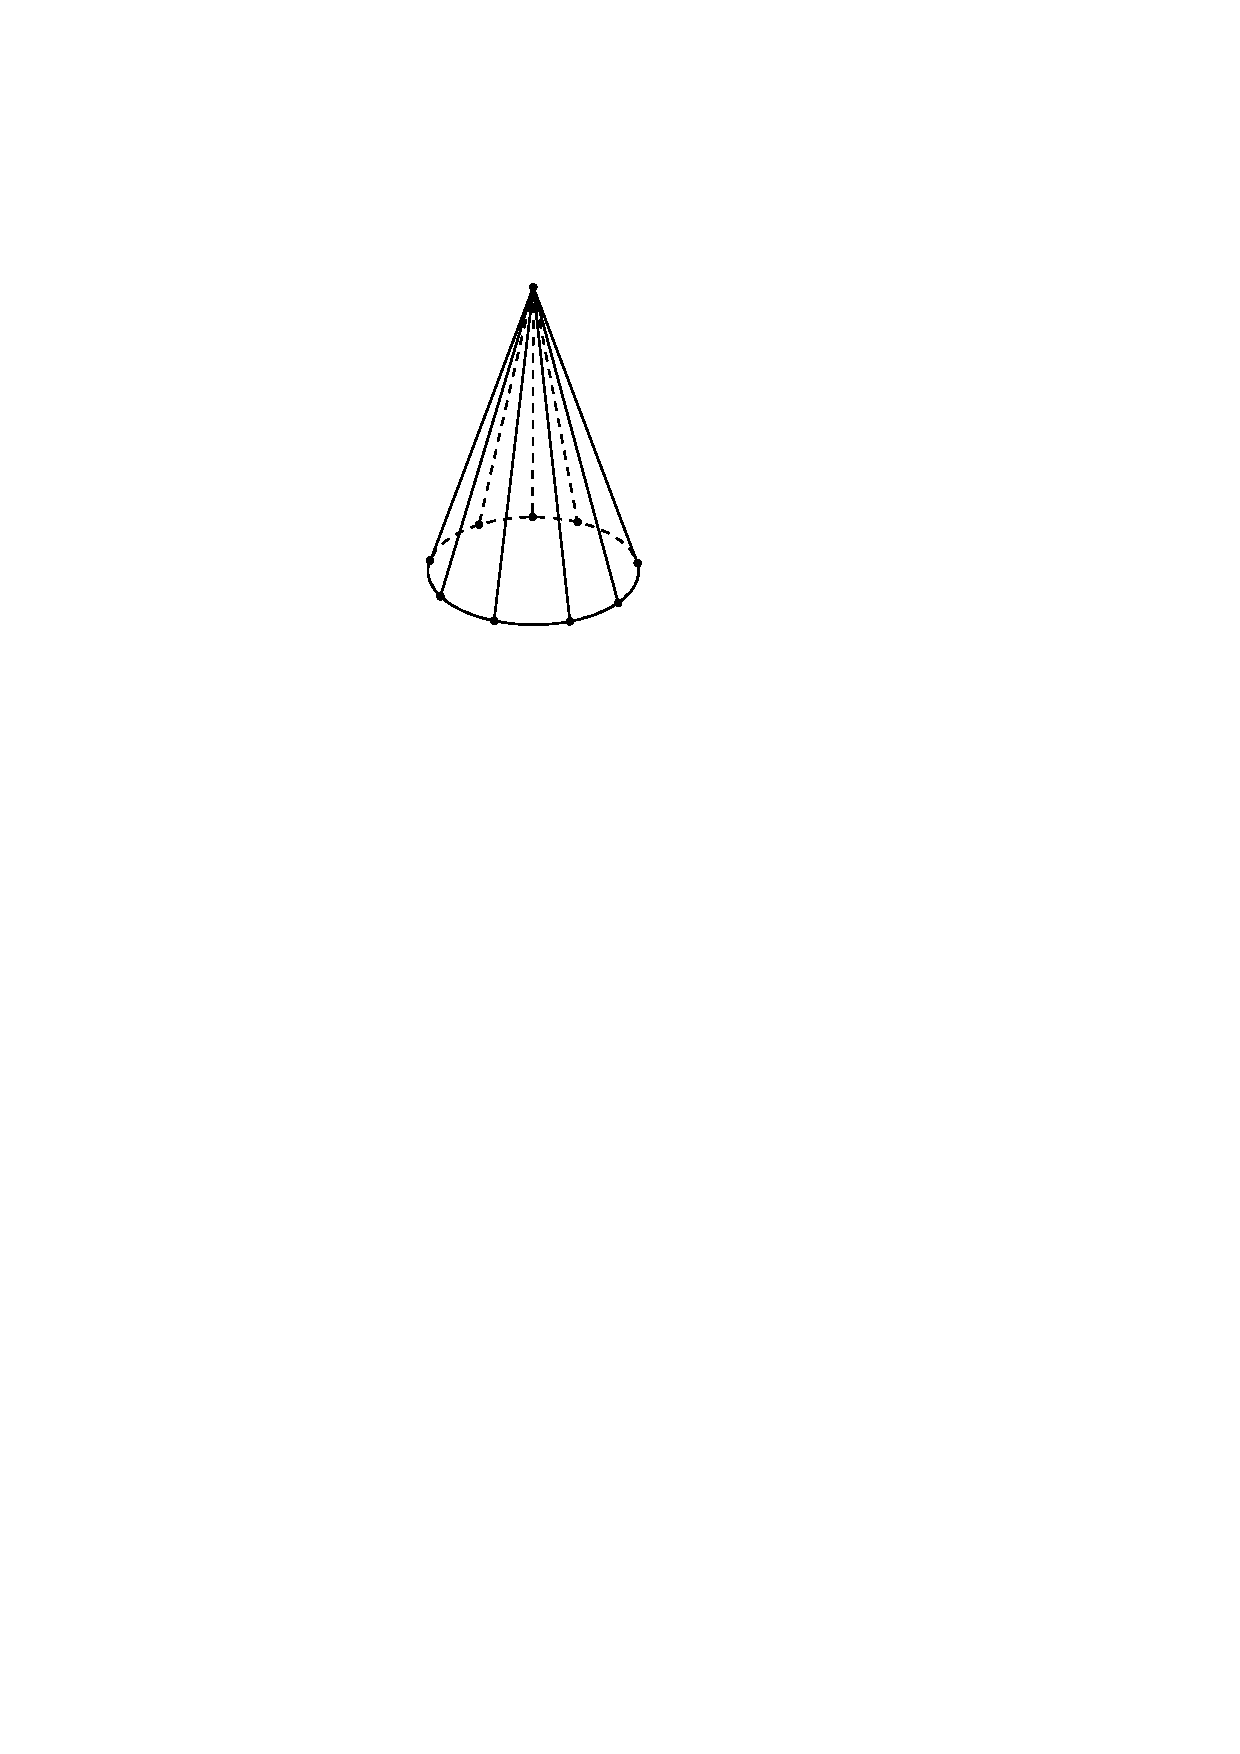
\includegraphics[width=.18\linewidth]{figs/diamond}\hspace{2cm}
    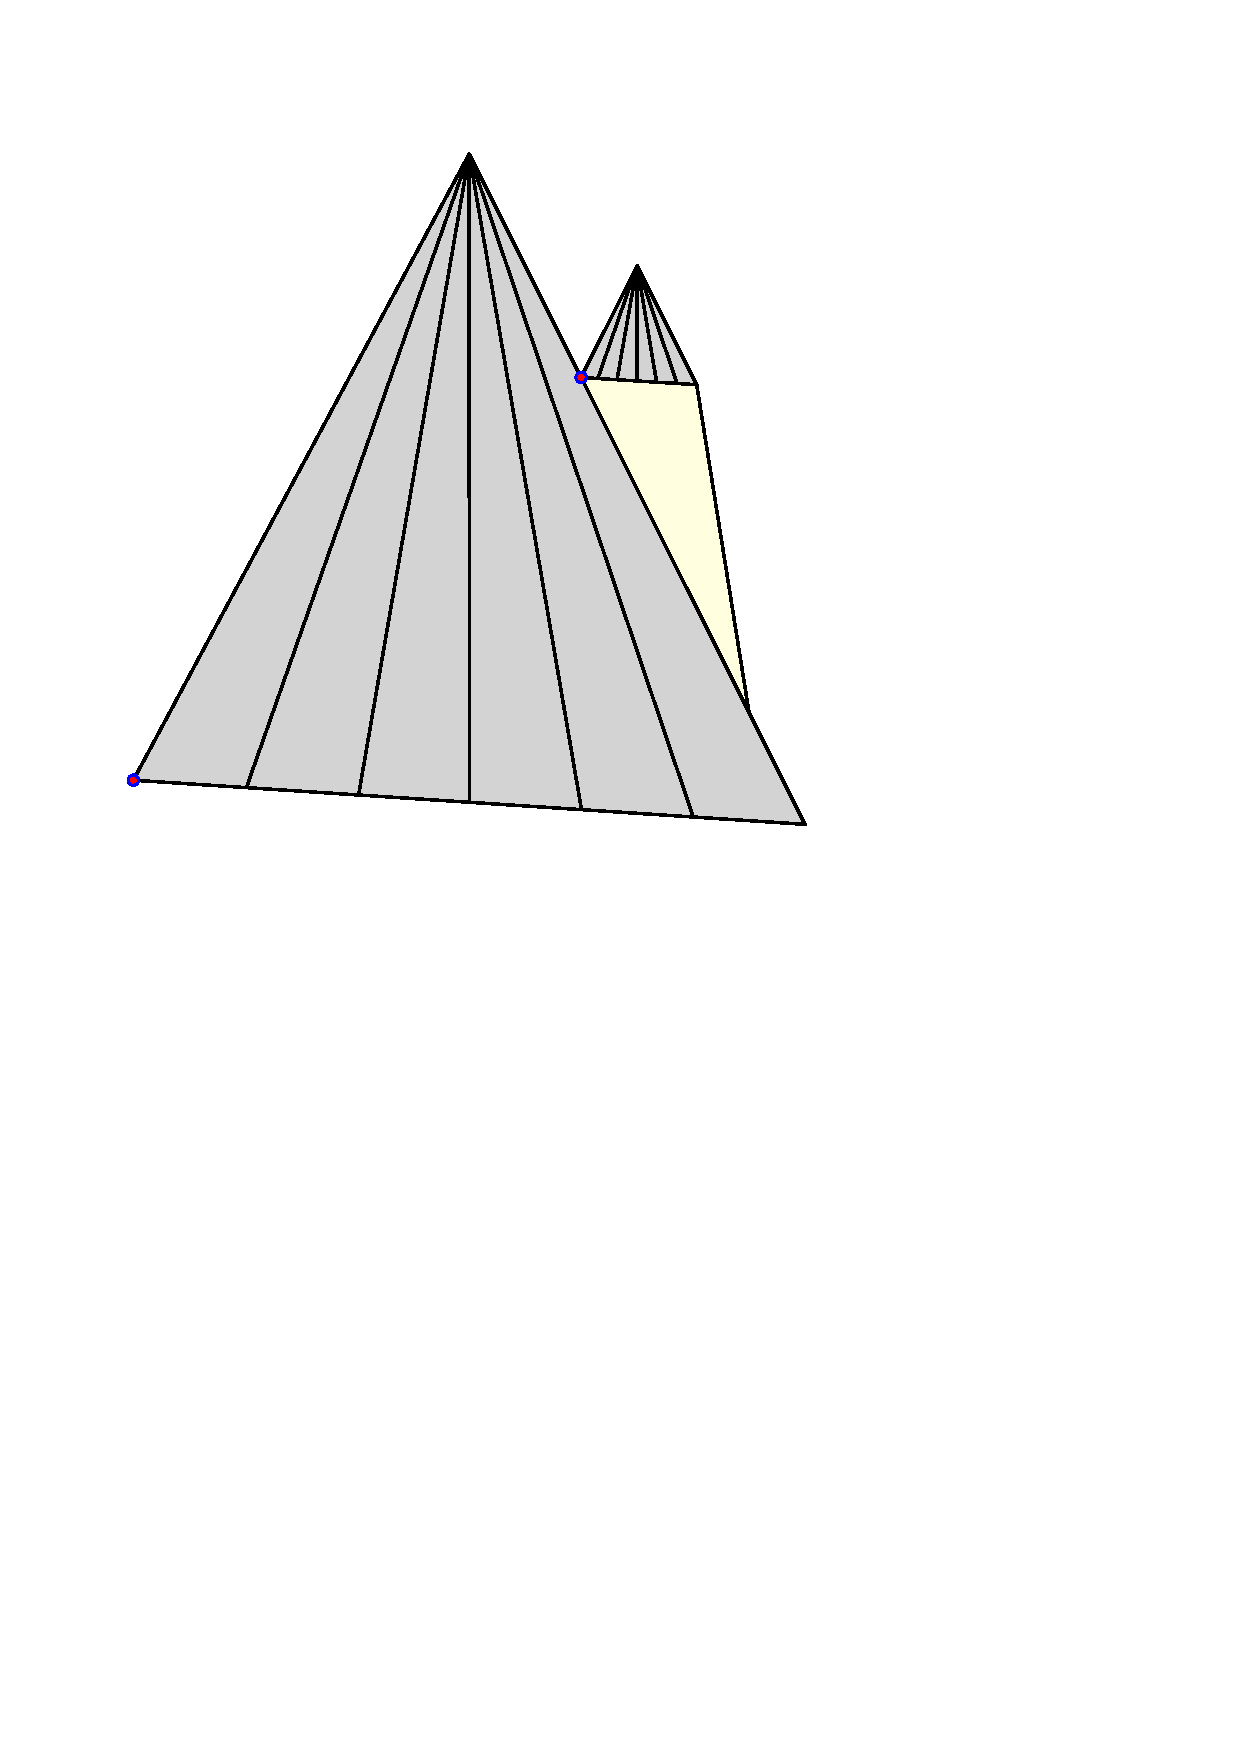
\includegraphics[width=.3\linewidth]{figs/cones}
%    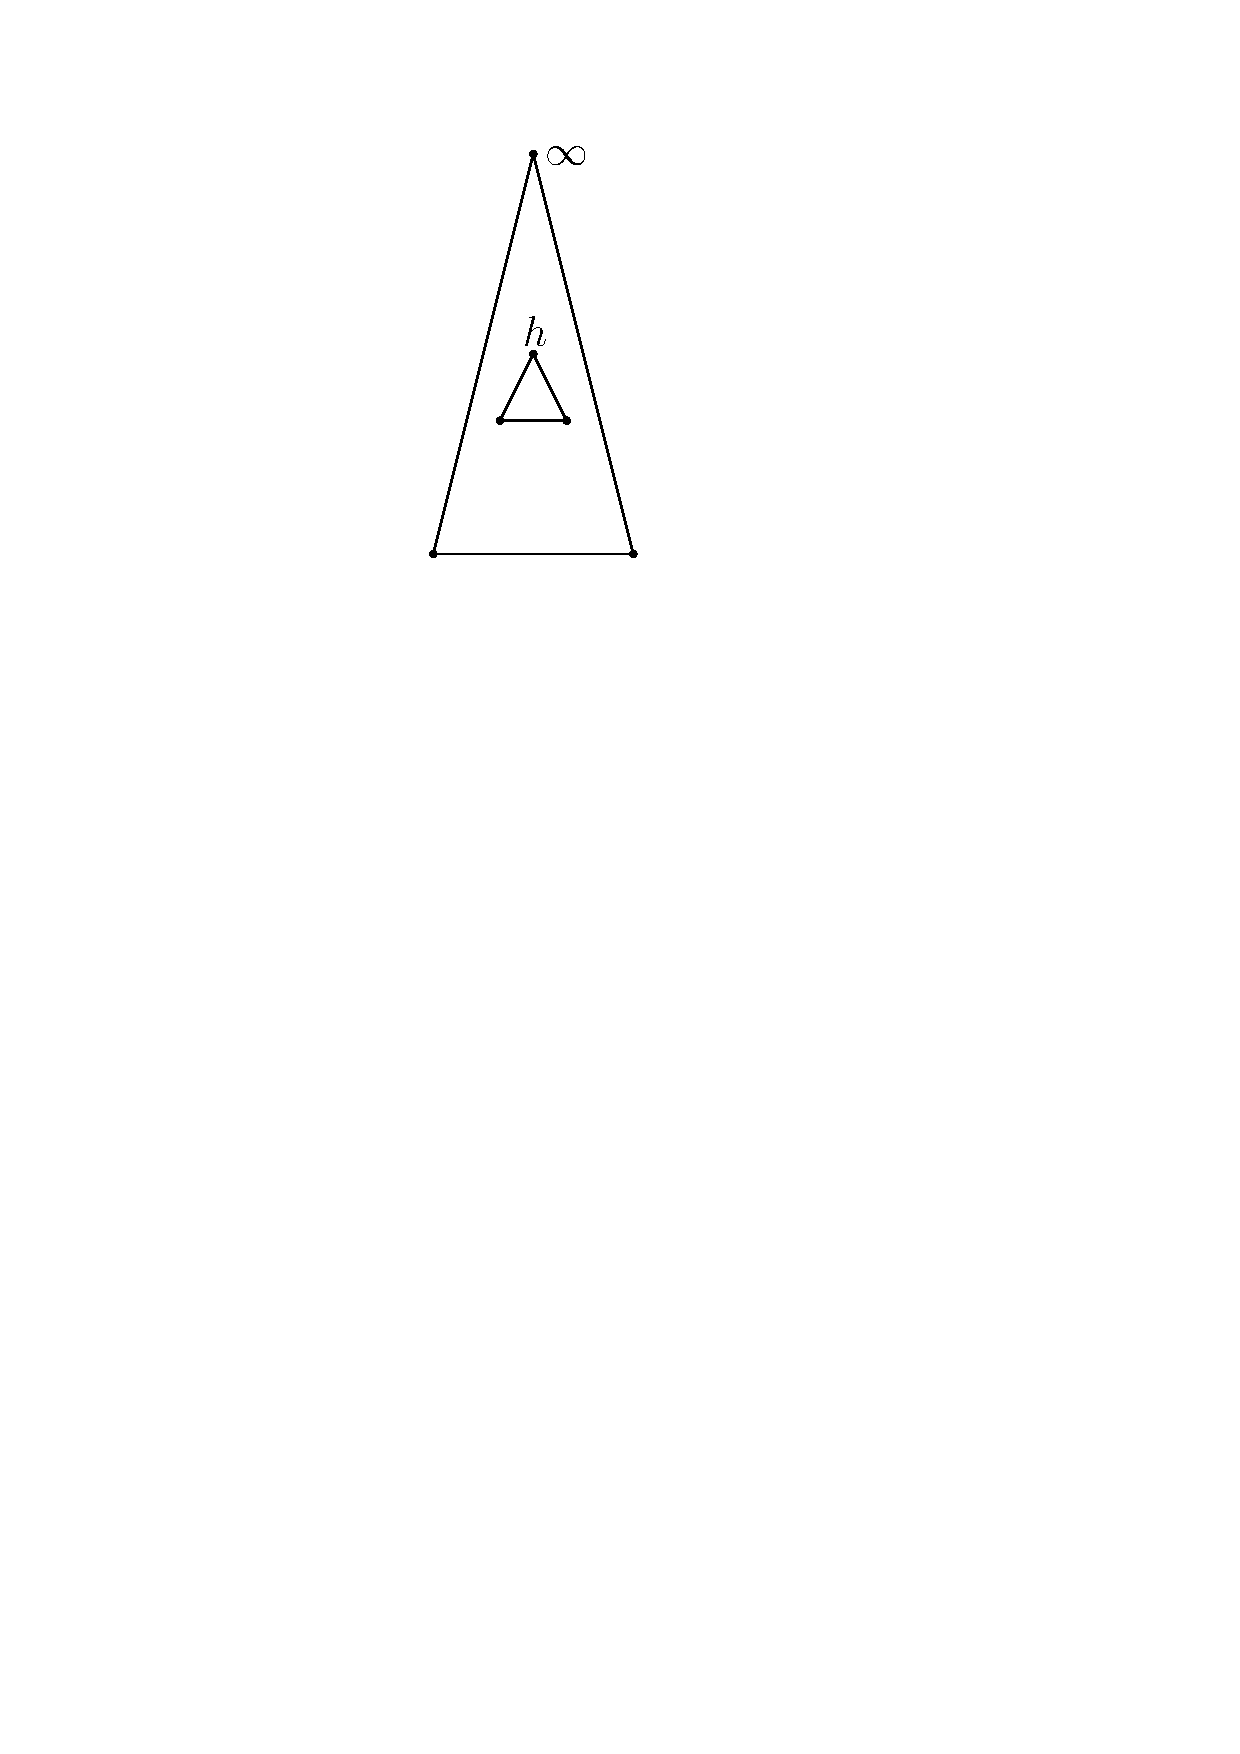
\includegraphics[width=.125\linewidth]{figs/topView}\hspace{2cm}
%    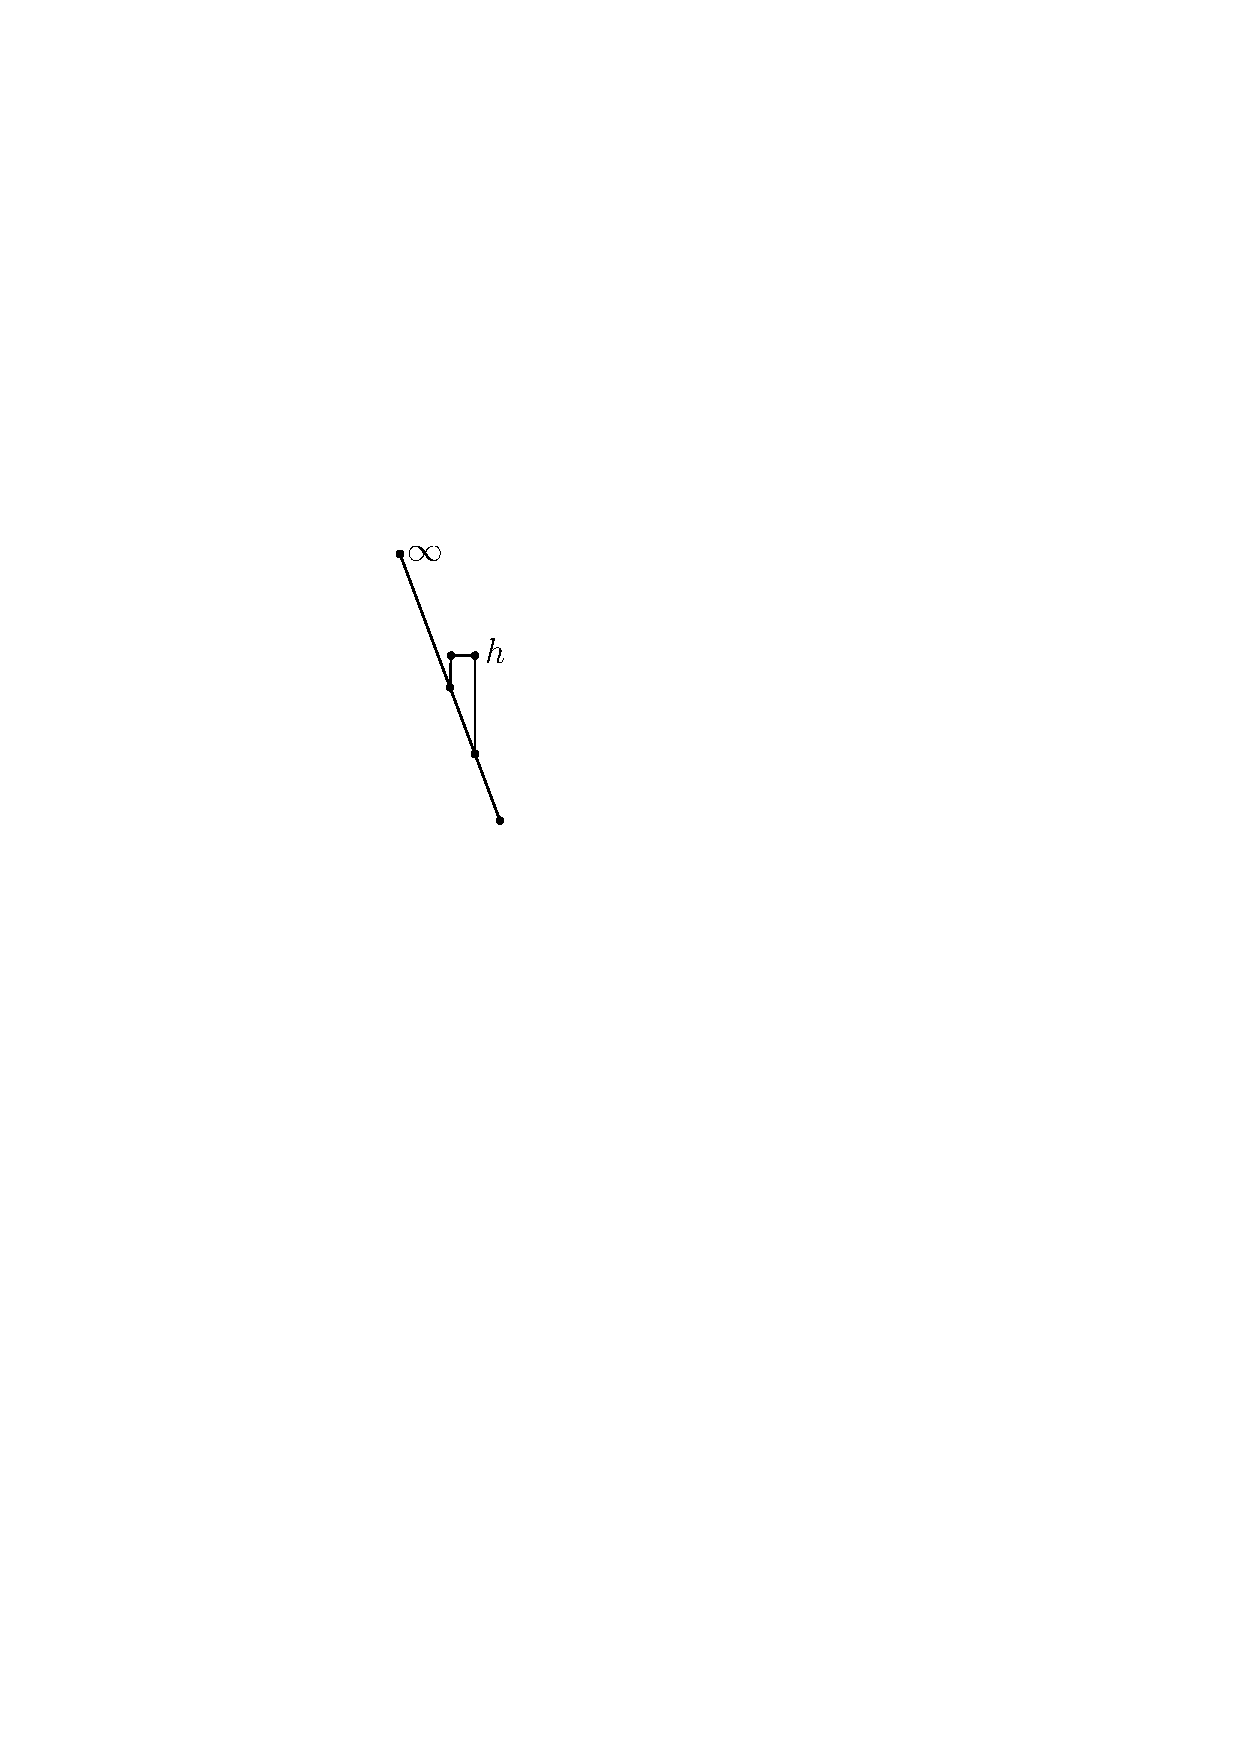
\includegraphics[width=.095\linewidth]{figs/sideView}
    \caption{Left: angled view of a diamond / Right: a parent and child diamond put together}
    \label{fig:diamond}
\end{figure}

\begin{lemma}
\label{lem:pathDecomp}
Fix any path decomposition $P$. There is a family of terrains, $\bF_P$, all with the same triangulation, 
such that $|\bF_P| = \Pi_{p_i\in P} (|p_i|-1)!$, and no two terrains in $\bF_P$ define the same join tree.
\end{lemma}


\begin{proof}
% We describe a simple triangulation, with heights specified for all vertices except for the saddles.  
 
%The main idea is that 
% this triangulation will be flexible enough to allow almost any assignment of heights to the saddles, thus defining a class of join trees 
% whose size is that described in the lemma statement. 
 We describe the basic building block of these terrains, which corresponds to a fixed path $p\in P$.  
 Informally, a \emph{diamond} is an upside down cone with $m$ triangular faces (see \Fig{diamond}). 
 Construct a slightly tilted cycle 
 of length $m$ with the two antipodal points at heights $1$ and $0$. These are called the anchor and trap of the diamond, respectively.
 The remaining $m-2$ vertices are evenly spread around the cycle and heights decrease monotonically when going from the anchor to the trap.
 Next, create an apex vertex at some appropriately large height, and add an edge to each vertex in the cycle. 


 Now we describe how to attach two different diamonds.  In this process, we glue the base of a scaled down ``child'' diamond on to a triangular cone face of the larger  ``parent'' diamond (see \Fig{diamond}).
 Specifically, the anchor of the child diamond is attached directly to a face of the parent diamond at some height $h$. The remaineder of the base of the child cone is then 
 extended down (at a slight angle) until it hits the face of the parent.
 
 The full terrain is obtained by repeatedly gluing diamonds. For each path $p_i\in P$, we create a diamond of size $|p_i|+1$.
 The two faces adjacent to the anchor are always empty, and the remaining faces are for gluing on other diamonds.
 (Note that diamonds have size $|p_i|+1$ since $|p_i|-1$ faces represent the joins of $p_i$, the apex represents the leaf, 
 and we need two empty faces next to the anchor.)
 Now we glue together diamonds of different paths in the same way the paths are connected in the shrub $\pathTree$ (see \Sec{shrubs}).  
 Specially, for two paths $p,q\in P$ where 
 $p$ is the parent of $q$ in $\pathTree$, we glue $q$ onto a face of the diamond for $p$ as described above.
 (Naturally for this construction to work, diamonds for a given path will be scaled down relative to the size of the diamond of their parent).
 By varying the heights of the gluing, we get the family of terrains.
 
 Observe now that the only saddle points in this construction are the anchor points.  Moreover, the only maxima are the apexes of the 
 diamonds.  We create a global boundary minimum by setting the vertices at the base of the diamond representing the root of $\pathTree$ all to the same height (and there are no other minima).  
 Therefore, the saddles on a given diamond will appear contiguously on a root to leaf path in the join tree of the terrain, where the leaf corresponds to the maxima of the diamond 
 (since all these saddles have a direct line of sight to this apex).  In particular, 
 this implies that, regardless of the heights assigned to the anchors, the join tree has a path decomposition whose corresponding shrub is equivalent to $\pathTree$.  
 
 There is a valid instance of this described construction for any relative ordering of the heights of the saddles on a given diamond.  
 In particular, there are $(|p_i|-1)!$ possible orderings of the heights of the saddles on the diamond for $p_i$, and hence $\Pi_{p_i\in P} (|p_i|-1)!$ possible 
 terrains we can build.  Each one of these functions will result in a different (labeled) join tree. All saddles on a given diamond will appear in sorted order in the join tree.
 So, any permutation of the heights on a given diamond corresponds to a permutation of the vertices along a path in $P$.
\end{proof}

Two path decompositions $P_1$ and $P_2$ (of potentially different complexes and/or height functions) are equivalent 
if: there is a 1-1 correspondence between the sizes of the constituent paths, and the shrubs are isomorphic.
%
%
%if their respective shrubs, $S_1$ and $S_2$, which has the property that for any node $v\in S_1$ corresponding to a path of 
%size $|v|$, $f(v)$ also corresponds to a path of size $|v|$. Note that for equivalent decompositions, $\sum_{p\in P_1} |p|\log|p| = \sum_{p\in P_2} |p|\log|p|$.

\begin{lemma}
\label{lem:cost}
For all $\MM \in \bF_P$, the total number of heap operations performed by $\build(\MM)$ is $O(\sum_{p\in P} |p|\log|p|)$.
\end{lemma}
\begin{proof}
%For any choice of $\MM \in \bF$, there is a path decomposition $\overline{P}(T)$ of the join tree equivalent to $\mathcal{P}$.
%Specifically, this is the decomposition where each path $p\in \overline{P}(T)$ consists exactly of the set of critical points (except for its anchor) from a given diamond. 
The primary ``non-determinism" of the algorithm is the initial painting constructed by $\init(\MM)$. 
We show that regardless of how paint spilling is done, the number of heap operations is bounded as above.

 Consider an arbitrary order of the initial paint spilling over the surface.
 Consider any join on a face of some diamond, which is the anchor point of some connecting child diamond.  
 The join has two up-stars, each of which has exactly one edge. Each edge connects to a maxima
 and must be colored by that maxima.
 Hence, the two colors touching this join (according to \Def{initialColoring})
 are the colors of the apexes of the child and parent diamond.  
% 
% Specifically, one of these edges connects directly to the apex of the parent diamond and so the join must get the color of this maxima.
% The other edge connects directly to the apex of the child diamond (this is why we left the faces adjacent to an anchor empty) and 
% so the second color is that of the maxima of the child diamond.
 
 Take any join $v$, with two children $w_1$ and $w_2$. Suppose $w_1$ and $v$ belong to the same path
 in the decomposition. The key is that any color from a maxima in the subtree at $w_2$ cannot touch
 any ancestor of $v$. This subtree is exactly the contour tree of the child diamond attached at $v$.
 The base of this diamond is completely contained in a face of the parent diamond. So all colors
 from the child ``drain off" to the base of the parent, and do not touch any joins on the parent diamond.
 
 Hence, $|H_v|$ is at most the size of the path in $P$ containing $v$. By \Lem{runTimeUpper}, the total number of heap operations
 is at most $\sum_v \log |H_v|$, completing the proof.
 
% 
% So let $c$ be the color of some maxima, $m$.  The above proven property of the coloring implies that in the join tree, the vertices for 
% which $c$ appears are exactly the vertices of the path in  $\overline{P}(T)$ corresponding $m$, as well as 
% the vertex to which the root of this path connects to (i.e. the anchor of the diamond of $m$).
% Now we show this implies $\overline{P}(T)$ is a maximum path decomposition.
% To see this, consider a vertex $v\in T$, and let $p$ be the path in $\overline{P}(T)$ which contain $v$. 
% Now $v$ has two children (if it is a join).  Let $c_1$ be the child which is in $p$, and $c_2$ the child which is the root of some adjacent path $p'$.  
% In order for $\overline{P}(T)$ to be the maximum path decomposition, we must show $|H_{c_1}|\geq |H_{c_2}|$.
% %(Note, to ensure a unique maximum path decomposition, one can break ties consistently by assigning some arbitrary but fixed ordering to the vertices.)
% %Now $v$ gets assigned two colors, one 
% %of which we know is the color assigned to all vertices in $p$ and the other is the one assigned to all the vertices of $p'$. 
% Observe that none of the colors in the subtree of $c_2$ appear below $v$.  Hence the heap at $c_2$ consists only of $v$.  
% On the other hand the heap of $c_1$ contains $v$, any other vertex of $p$ below $v$, and the vertex to which the root of $p$ is adjacent to, 
% and hence $|H_{c_1}|\geq |H_{c_2}|$.
\end{proof}

The following is the equivalent of \Thm{main-lb} for join trees, and immediately follows from
the previous lemmas.
%Call a cost $C$ join tree valid if $C = cost_{\jc}(f)$ for some $f$ defined over a given complex $\MM$.

\begin{theorem}\label{thm:joinLB}
Consider a rooted tree $T$ and an arbitrary path decomposition $P$ of $T$.
There is a family $\bF_P$ of terrains such that any algebraic decision
tree computing the contour tree (on $\bF_P$) requires $\Omega(\sum_{p \in P} |p|\log |p|)$ time.
Furthermore, our algorithm makes $O(\sum_{p \in P} |p|\log |p|)$ comparisons on all these instances.
%
%Consider the set of functions $\bF_C$ that all have the same join tree valid cost $C$.  
%Any height function decision tree that correctly computes
%the join tree on all of $\bF_C$, has an average case (uniform over $\bF_C$) running time of $\Omega(C)$.
\end{theorem}

\begin{proof}
The proof is a basic entropy argument. Any algebraic decision tree that is correct on all of $\bF_P$
must distinguish all inputs in this family. By Stirling's approximation, the depth of this tree is $\Omega(\sum_{p_i\in P} |p_i|\log|p_i|)$.
\Lem{cost} completes the proof.
%
%
% If $C$ is a join tree valid cost then there some $f$ such that $\cost_{\jc}(f)=\sum_{p\in P(f)} |p|\log|p|$.
% By the above lemmas, there is then a set $\bF$ of $\Pi_{p_i\in P} |p_i|!$ functions, such that for any $g\in \bF$, $C= \cost(g)$.  
% (Specifically, each sorted ordering of the relative height values of the saddles on each diamond yields a function in this class.)
% Hence $\bF\subseteq \bF_C$, and so any height function decision tree for the set $\bF_C$ must distinguish between these possibilities, and therefore must 
% have $\Pi_{p_i\in P} |p_i|!$ leaves.  Hence by Stirling's approximation, the average depth in this tree is $\Omega(\sum_{p_i\in P} |p_i|\log|p_i|)$.
\end{proof}

\subsection{Contour Trees}
We first generalize previous terms to the case of contour trees.
In this section $T$ will denote an arbitrary contour tree with every internal vertex of degree $3$.
%and the height function defined over the vertex set is such that every internal vertex in either a split or join 
%(i.e. at most $2$ neighbors lie above or below it).

%We need to generalize the definition of path decompositions, which previously were only defined for rooted trees.
%Again we define a path decomposition as a partition of the vertices into 
%disjoint leaf paths (i.e. each path is monotonic in height and contains a leaf). 
For simplicity we now restrict our attention to path decompositions 
consistent with the raining procedure described in \Sec{rain} 
(more general decompositions can work, but it is not needed for our purposes).

\begin{definition}
\label{def:path2} A path decomposition, $P(T)$, is called \emph{rain consistent} if its paths can be obtained as follows.
Perform an downward BFS from an arbitrary maxima $v$ in $T$, and mark all vertices encountered.  
Now recursively run a directional BFS from all vertices adjacent to the current marked set.  
Specifically, for each BFS run, make it an downward BFS if it is at an odd height in the recursion tree and upward otherwise.  

This procedure partitions the vertex set into disjoint rooted subtrees of $T$, based on which BFS marked a vertex.  
For each such subtree, now take any partition of the vertices into leaf paths.\footnote{Note that the subtree  
of the initial vertex is rooted at is a maxima.  For simplicity we require that the path this vertex belongs to 
also contains a minima.}
\end{definition}

%
%Consider our algorithm on a fixed $(f,\MM)$.  First we run $\rain(x,\MM)$ to partition the input 
%into extreme dominant complexes.  To make this partition uniquely defined lets say that the initial vertex $x$
%that rain is called from is the global maximum in the input (note that given a specific $x$ the partition is uniquely defined).
%Let $\MM_1, \dots, \MM_k$ be the set of produced subcomplexes, and let $f_i$ be the restriction of $f$ to $\MM_i$.
%Now on each of the $(f_i,\MM_i)$ we run the $\paint$ procedure to compute the join tree of $(f_i, \MM_i)$.
%As described in the previous section, this painting procedure defines a maximum path decomposition with 
%and associated cost, $\cost_{\jc}(f_i) = \sum_{p\in P_i} |p|\log |p|$.  
%It is not hard to see that the union of these paths decomposition $P= \cup_{i=1}^k P_i$ defines 
%a rain consistent path decomposition of the contour tree for $(f,\MM)$.  
%In particular for a fixed $\MM$, $f$ defines a specific path decomposition $P=P(f)$, which we call the \emph{rain consistent maximum path decomposition}, 
%and we write $\cost(f) = \sum_{p\in P} |p|\log |p|$.

The following is analogous to \Lem{pathDecomp}, and in particular uses it as a subroutine.

\begin{lemma}
\label{lem:pathDecomp2}
Let $P$ be any rain consistent path decomposition of some contour tree. 
There is a family of terrains, $\bF_P$, all with the same triangulation, 
such that the size of $\bF_P$ is $\Pi_{p_i\in P} (|p_i|-1)!$, and no two terrains in $\bF_P$ define the same contour tree.
\end{lemma}
\begin{proof}
 As $P$ is rain consistent, the paths can be partitioned into sets $P_1, \dots, P_k$, where $P_i$ is the set of all paths with 
 vertices from a given BFS, as described in \Def{path2}.  Specifically, let $T_i$ be the subtree of $T$ corresponding to $P_i$ and 
 let $r_i$ be the root vertex of this subtree.  
 Note that the $P_i$ sets naturally define a tree where $P_i$ is the parent of $P_j$ if $r_i$ (i.e. the root of $T_i$) is adjacent to a vertex in $P_j$.  
 
 As the set $P_i$ is a path decomposition of a rooted binary tree $T_i$, the terrain construction of \Lem{pathDecomp} for $P_i$ is well defined.  
 Actually the only difference is that here the rooted tree is not a full binary tree, and so some of the (non-achor adjacent) faces of the constructed diamonds will be blank.  
 Specifically, these blank faces correspond to the adjacent children of $P_i$, and they tell us how to connect the terrains of the different $P_i$'s.
 
 So for each $P_i$ construct a terrain as described in \Lem{pathDecomp}.  Now each $T_i$ is (roughly speaking) a join or a split tree, depending on 
 whether the BFS which produced it was an upward or downward BFS, respectively.  As the construction in \Lem{pathDecomp} was for join trees, each terrain 
 we constructed for a $P_i$ which came from a split tree, must be flipped upside down.
 Now we must described how to glue the terrains together.
  
 \begin{figure}[h]\centering
    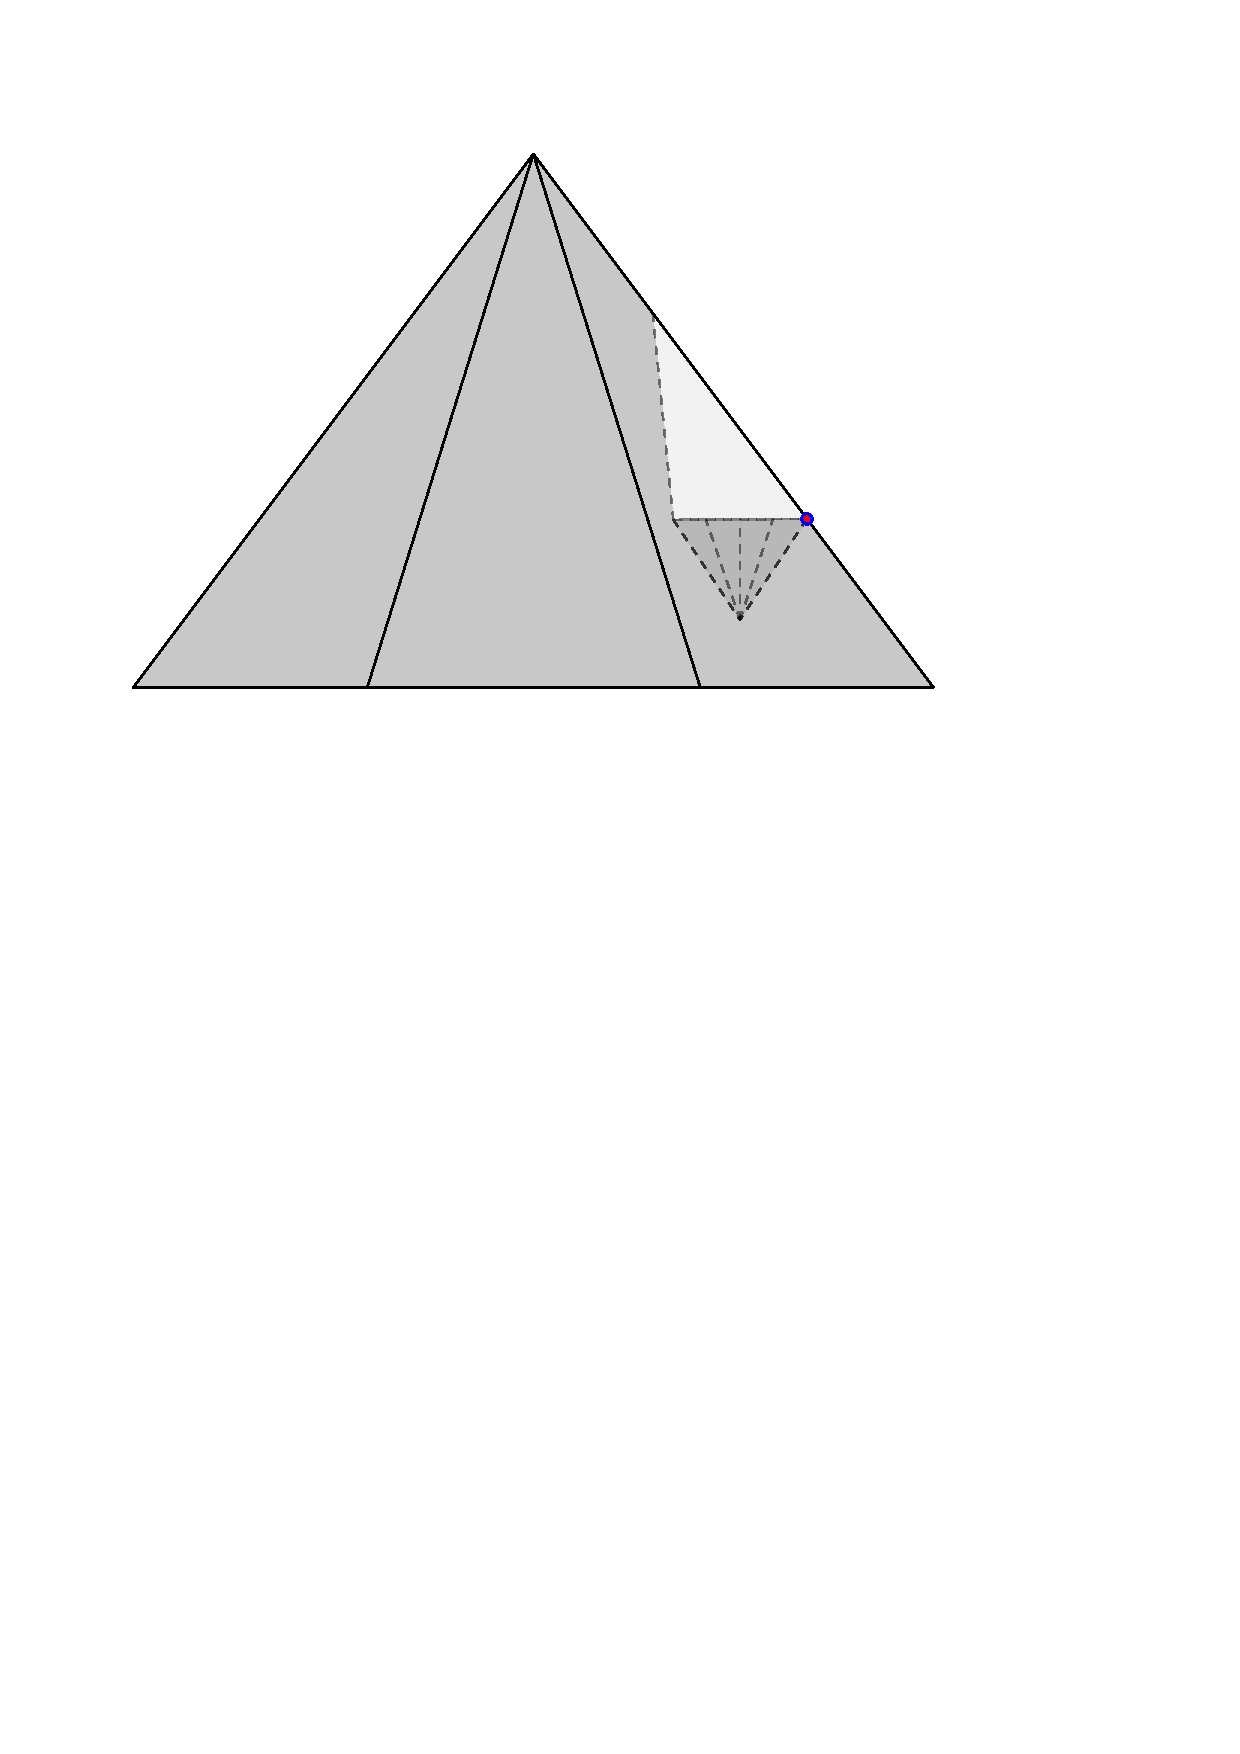
\includegraphics[width=.28\linewidth]{figs/cones2}
    \caption{A child diamond attached to a parent diamond with opposite orientation.}
    \label{fig:diamond2}
\end{figure} 
  
 By construction, the diamonds corresponding to the paths in $P_i$ are connected 
 into a tree structure (i.e. corresponding to the shrub of $P_i$).  Therefore the bottoms of all these diamonds are covered except for the one corresponding 
 to the path containing the root $r_i$.  
 If $r_i$ corresponds to the initial maxima that the rain consistent path decomposition was defined from, then this will be flat and corresponds to the global outer face.
 Otherwise, $P_i$ has some parent $P_j$ in which case we connect the bottom of the diamond for $r_i$ to a free face of a diamond in the construction for $P_j$, specifically, the face corresponding to the 
 vertex in $T$ which $r_i$ is adjacent to. This gluing is done in the same manner as in \Lem{pathDecomp}, attaching the anchor for the root of $P_i$ directly the corresponding face of $P_j$, except that now $P_i$ and $P_j$ have opposite orientations.  See \Fig{diamond2}.
 
 Just as in \Lem{pathDecomp} we now have one fixed terrain structure, such that each different relative ordering of the heights of the join and split vertices 
 on each diamond produces a surface with a distinct contour tree.  The specific bound on the size of $\bF_P$, defining these distinct contour trees, follows by applying the 
 bound from \Lem{pathDecomp} to each $P_i$.
\end{proof}




\begin{lemma}
For all $\MM \in \bF_P$, the number of heap operations is $\Theta(\sum_{p\in P} |p|\log |p|)$
\end{lemma}
\begin{proof}
 This lemma follows immediately from \Lem{cost}.  The heap operations can be partitioned into the
 operations performed in each $P_i$.
 Apply \Lem{cost} to each of the $P_i$ separately and take the sum.
\end{proof}

We now restate \Thm{main-lb}, which follows immediately from an entropy argument, analogous to \Thm{joinLB}.

\begin{theorem} 
Consider any rain consistent path decomposition $P$. There exists a family $\bF_P$ of terrains ($d=2$) with the following properties.
Any contour tree algorithm makes $\Omega(\sum_{p \in P} |p|\log |p|)$ comparisons in the worst case over $\bF_P$.
Furthermore, for any terrain in $\bF_P$, our algorithm makes $O(\sum_{p \in P} |p|\log |p|)$ comparisons.
\end{theorem}

%
%
%Call a cost $C$ valid if $C = cost(f)$ for some $f$ defined over a given complex $\MM$.
%For the same reason that \Thm{joinLB} followed from \Lem{pathDecomp} and \Lem{cost}, we now have the following. 
%
%\begin{theorem}
%Consider the set of functions $\bF_C$ that all have the same valid cost $C$.  
%Any height function decision tree that correctly computes
%the contour tree on all of $\bF_C$, has an average case (uniform over $\bF_C$) running time of $\Omega(C)$.
%\end{theorem}

\begin{remark}
 Note that for the terrains described in this section, the number of critical points is within a constant factor of 
 the total number of vertices.  In particular, for this family of terrains, all previous algorithms required $\Omega(n\log n)$ time.
\end{remark}




% \section{Temp}
% Given a contour tree we allow any path decomp, as long as each path contains a maxima or minima (or both).
% We call a path $p$ in the decomp a min (resp. max) path if it contains a minima (resp. maxima) (note a path can be both).
% For every path we create a cylinder with $m$ faces for $p$, where $m$ is the number of non-leaf vertices in $p$ (either $|p|-1$ or $|p|-2$).  
% If $p$ has a maxima we put a top cone cap on the cylinder, and if it contains a manima then put a bottom cone cap (i.e. the cap represents the maxima or minima).
% 
% Every edge $e$ in $T$, but not in a path decomp. tells us how to glue together cylinders.  Let $u$ be the upper endpoint of $e$ and $l$ the lower endpoint.
% 
% First we ``remove'' all edges $e$ such that $u$ is adjacent to a max path and $l$ adjacent to a min path by joining the free ends of the respective cylinder together.
% Hence we can assume no such edges exist.  Now we have three cases:
% 
% \begin{enumerate}[{Case} 1]
%  \item 
% $l$ is adjacent to a min path:\newline
% Note in this case the path containing $u$ must be a min path.
% In this case connect the bottom of the cylinder for the path containing $l$ into a face of the cylinder for the path containing $u$.
% \item
% $l$ is adjacent to a max path and $u$ is adjacent to a max path:\newline
% In this case connect the bottom of the cylinder for the path containing $u$ into a face of the cylinder for the path containing $l$.
% \item
% $l$ is adjacent to a max path and $u$ is adjacent to a min path:\newline
% Connect a face of the cylinder for the $u$ path (using a split) to a face of the cylinder for the $l$ path (using a join).
% \end{enumerate}
}


\paragraph{Acknowledgements.}
We thank Hsien-Chih Chang, Jeff Erickson, and Yusu Wang for numerous useful discussions. This work is
supported by the Laboratory Directed Research and Development
(LDRD) program of Sandia National Laboratories. Sandia National
Laboratories is a multi-program laboratory managed and operated
by Sandia Corporation, a wholly owned subsidiary of Lockheed
Martin Corporation, for the U.S. Department of Energy�s National
Nuclear Security Administration under contract DE-AC04-94AL85000.


\bibliographystyle{alpha}
\bibliography{contour}





%%%%%%%%%%%%%%%%%%%%%%%%%%%%%%%%%%%%%%%%%%%%%%%%%%%%%%%%%%%%%%%%%%%%%%%%%
%%%%%%%%%%%%%%%%%%%%%%%%%%%%%%%%%%%%%%%%%%%%%%%%%%%%%%%%%%%%%%%%%%%%%%%%%
%%%%%%%%%%%%%%%%%%%%%%%%%%%%%%%%%%%%%%%%%%%%%%%%%%%%%%%%%%%%%%%%%%%%%%%%%
%%%%%%%%%%%%%%%%%%%%%%%%%%%%%%%%%%%%%%%%%%%%%%%%%%%%%%%%%%%%%%%%%%%%%%%%%
%%%%%%%%%%%%%%%%%%%%%%%%%%%%%%%%%%%%%%%%%%%%%%%%%%%%%%%%%%%%%%%%%%%%%%%%%
%%%%%%%%%%%%%%%%%%%%%%%%%%%%%%%%%%%%%%%%%%%%%%%%%%%%%%%%%%%%%%%%%%%%%%%%%
%
%
%end of writup
%
%
%%%%%%%%%%%%%%%%%%%%%%%%%%%%%%%%%%%%%%%%%%%%%%%%%%%%%%%%%%%%%%%%%%%%%%%%%
%%%%%%%%%%%%%%%%%%%%%%%%%%%%%%%%%%%%%%%%%%%%%%%%%%%%%%%%%%%%%%%%%%%%%%%%%
%%%%%%%%%%%%%%%%%%%%%%%%%%%%%%%%%%%%%%%%%%%%%%%%%%%%%%%%%%%%%%%%%%%%%%%%%
%%%%%%%%%%%%%%%%%%%%%%%%%%%%%%%%%%%%%%%%%%%%%%%%%%%%%%%%%%%%%%%%%%%%%%%%%
%%%%%%%%%%%%%%%%%%%%%%%%%%%%%%%%%%%%%%%%%%%%%%%%%%%%%%%%%%%%%%%%%%%%%%%%%
%%%%%%%%%%%%%%%%%%%%%%%%%%%%%%%%%%%%%%%%%%%%%%%%%%%%%%%%%%%%%%%%%%%%%%%%%







\appendix


\end{document}
